\documentclass[12pt,a4paper]{report}
\usepackage{dissertation}
\usepackage{listings}
\usepackage{tikz}
\usepackage{xcolor}
\usepackage{array}
\usepackage{amsmath,amssymb}
\usepackage{colortbl}
\usepackage[utf8]{inputenc}
\usepackage{subcaption}
\usepackage{todonotes}
\makeglossaries
\makeindex

%\logo{EAAD}{School of Architecture, Art and Design}{}
%\logoB{EAAD}{School of Architecture, Art and Design}{}

%\logo{EC}{School of Sciences}{}
%\logoB{EC}{School of Sciences}{}

%\logo{ED}{Law School}{}
%\logoB{ED}{Law School}{}

\logo{EE}{School of Engineering}{}
\logoB{EE}{School of Engineering}{}

%\logo{EEG}{School of Economics and Management}{}
%\logoB{EEG}{School of Economics and Management}{}

%\logo{ELACH}{School of Letters, Arts and Human Sciences}{}
%\logoB{ELACH}{School of Letters, Arts and Human Sciences}{}

%\logo{EM}{Medical school}{}
%\logoB{EM}{Medical school}{}

%\logo{EP}{School of Psychology}{}
%\logoB{EP}{School of Psychology}{}

%\logo{ESE}{Higher School of Nursing}{}
%\logoB{ESE}{Higher School of Nursing}{}

%\logo{I3Bs}{Research Institute on Biomaterials,}{Biodegradables and Biomimetics}
%\logoB{I3Bs}{Research Institute on Biomaterials,}{Biodegradables and Biomimetics}

%\logo{ICS}{Institute of Social Sciences}{}
%\logoB{ICS}{Institute of Social Sciences}{}

%\logo{IE}{Institute of Education}{}
%\logoB{IE}{Institute of Education}{}

\author{Alexandre de Jesus Sousa e Silva}

\titleA{Analysis of families of Real Time Systems}
\titleB{with IMITATOR}



\masters{Master’s Dissertation in Physics Engineering}
%\area{Area of specialization}
\supervisor{José Miguel Paiva Proença}
\cosupervisor{Renato Jorge Araújo Neves}

\tcbuselibrary{listingsutf8}
\newtcolorbox{commandline}{
  colback=black,
  coltext=green!60!black,
  boxrule=0pt,
  arc=0mm,
  outer arc=0mm,
  left=2pt,
  right=2pt,
  top=2pt,
  bottom=2pt,
  boxsep=2pt,
  fontupper=\ttfamily,
  enhanced,
  sharp corners
}

\bibpunct[,]{(}{)}{;}{a}{,}{,}

\newcommand{\imitator}[1]{\texttt{\textbf{\textcolor{green!30!black}{#1}}}}

\definecolor{keywordcolor}{RGB}{0,0,255}      % Azul para palavras-chave
\definecolor{commentcolor}{RGB}{0,128,0}      % Verde para comentários
\definecolor{stringcolor}{RGB}{163,21,21}     % Vermelho escuro para strings
\definecolor{backgroundcolor}{RGB}{240,240,240}

\lstdefinelanguage{UPPAAL}
{
    keywords={var, clock, discrete, bool, constant, parameter, automaton, sync, loc, invariant, when, do, goto, end, init},
    keywordstyle=\color{keywordcolor}\bfseries,
    morecomment=[s]{(*}{*)},
    % morecomment=[l]{(*},
    % morecomment=[r]{*)},
    commentstyle=\color{commentcolor}\textit,
    morestring=[b]",
    stringstyle=\color{stringcolor},
    basicstyle=\ttfamily\small,
    backgroundcolor=\color{backgroundcolor},
    tabsize=4,
    showstringspaces=false,
    breaklines=true
}

\lstdefinelanguage{MOREUPPAAL}
{
    keywords={var, const, int, clock, discrete, bool, constant, parameter, automaton, sync, loc, invariant, when, do, goto, end, init},
    keywordstyle=\color{keywordcolor}\bfseries,
    % morecomment=[s]{(//}{//)},
    morecomment=[l]{//},
    % morecomment=[l]{(*},
    % morecomment=[r]{*)},
    commentstyle=\color{commentcolor}\textit,
    morestring=[b]",
    stringstyle=\color{stringcolor},
    basicstyle=\ttfamily\small,
    backgroundcolor=\color{backgroundcolor},
    tabsize=4,
    showstringspaces=false,
    breaklines=true
}

% \includeonly{
%   chapters/Introduction,
%   chapters/StateOfTheArt
%   chapters/PlannedSchedule,
%   chapters/Imitator_Backend,
%   chapters/TowardsAUppexInterface,
%   chapters/ConclusionsAndFutureWork,
%   appendices/SupportWork,
% }

\begin{document}
\setlength{\parindent}{0em}

%-- Covers
\begin{titlepage}
\color{PANTONECoolGray7C}
\thelogo
\leading{20.4pt}
{\Large
\theauthor
\\
%
\\
\textbf{\thetitleA}
\\
\textbf{\thetitleB}
\\
\textbf{\thetitleC}
}

\vspace*{\fill}
{\footnotesize \myear}
\end{titlepage}

\null
\thispagestyle{empty}
\pagecolor{PANTONECoolGray7C}
\afterpage{\nopagecolor}
\newpage

\begin{titlepage}
\color{PANTONECoolGray7C}
\thelogoB
\leading{20.4pt}
{\Large
\theauthor
\\
%
\\
\textbf{\thetitleA}
\\
\textbf{\thetitleB}
\\
\textbf{\thetitleC}
}

\vspace{55.2mm}
\leading{16.8pt}
{\large
\themasters
\\
\thearea
Dissertation supervised by
\\
\textbf{\thesupervisor}
\\
\thecosupervisor}

\vspace*{\fill}
{\footnotesize \myear}
\end{titlepage}

%-- Document setup
\newgeometry{right=25mm, left=25mm, top=25mm, bottom=25mm}
\pagenumbering{roman}

\setlength{\parskip}{0pt}
\setlength{\parindent}{1.5em}

% \chapter*{Copyright and Terms of Use for Third Party Work}
\setlength{\parskip}{1em}
%\noindent
%This dissertation reports on academic work that can be used by third parties as long as the internationally accepted standards and good practices are respected concerning copyright and related rights.

%\noindent
%This work can thereafter be used under the terms established in the license below.

%\noindent
%Readers needing authorization conditions not provided for in the indicated licensing should contact the author through the RepositóriUM of the University of Minho.

%\section*{License granted to users of this work:}

%\textit{[Caso o autor pretenda usar uma das licenças Creative Commons, deve escolher e deixar apenas um dos seguintes ícones e respetivo lettering e URL, eliminando o texto em itálico que se lhe segue. Contudo, é possível optar por outro tipo de licença, devendo, nesse caso, ser incluída a informação necessária adaptando devidamente esta minuta]}

%\noindent
%
\includegraphics[]{images/CCBY.png}
%\\
%\textbf{CC BY}
%\\
%\url{https://creativecommons.org/licenses/by/4.0/}
%\textit{[Esta licença permite que outros distribuam, remixem, adaptem e criem a partir do seu trabalho, mesmo para fins comerciais, desde que lhe atribuam o devido crédito pela criação original. É a licença mais flexível de todas as licenças disponíveis. É recomendada para maximizar a disseminação e uso dos materiais licenciados.]}

%--

%\noindent
%
\includegraphics[]{images/CCBYSA.png}
%\\
%\textbf{CC BY-SA}
%\\
%\url{https://creativecommons.org/licenses/by-sa/4.0/}
%\textit{[Esta licença permite que outros remisturem, adaptem e criem a partir do seu trabalho, mesmo para fins comerciais, desde que lhe atribuam o devido crédito e que licenciem as novas criações ao abrigo de termos idênticos. Esta licença costuma ser comparada com as licenças de software livre e de código aberto «copyleft». Todos os trabalhos novos baseados no seu terão a mesma licença, portanto quaisquer trabalhos derivados também permitirão o uso comercial. Esta é a licença usada pela Wikipédia e é recomendada para materiais que seriam beneficiados com a incorporação de conteúdos da Wikipédia e de outros projetos com licenciamento semelhante.]}

%--

%\noindent
%
\includegraphics[]{images/CCBYND.png}
%\\
%\textbf{CC BY-ND}
%\\
%\url{https://creativecommons.org/licenses/by-nd/4.0/}
%\textit{[Esta licença permite que outras pessoas usem o seu trabalho para qualquer fim, incluindo para fins comerciais. Contudo, o trabalho, na forma adaptada, não poderá ser partilhado com outras pessoas e têm que lhe ser atribuídos os devidos créditos.]}

%--

%\noindent
%
\includegraphics[]{images/CCBYNC.png}
%\\
%\textbf{CC BY-NC}
%\\
%\url{https://creativecommons.org/licenses/by-nc/4.0/}
%\textit{[Esta licença permite que outros remisturem, adaptem e criem a partir do seu trabalho para fins não comerciais, e embora os novos trabalhos tenham de lhe atribuir o devido crédito e não possam ser usados para fins comerciais, eles não têm de licenciar esses trabalhos derivados ao abrigo dos mesmos termos.]}

%--

%\noindent
%
\includegraphics[]{images/CCBYNCSA.png}
%\\
%\textbf{CC BY-NC-SA}
%\\
%\url{https://creativecommons.org/licenses/by-nc-sa/4.0/}
%\textit{[Esta licença permite que outros remisturem, adaptem e criem a partir do seu trabalho para fins não comerciais, desde que lhe atribuam a si o devido crédito e que licenciem as novas criações ao abrigo de termos idênticos.]}

%--

\noindent

This dissertation reports on academic work that can be used by third parties as long as the
internationally accepted standards and good practices are respected concerning copyright and related rights.

This work can thereafter be used under the terms established in the license below.

Readers needing authorization conditions not provided for in the indicated licensing should contact the author through the RepositóriUM of the University of Minho.
\paragraph{}



\includegraphics[]{images/CCBYNCND.png}
\\
\textbf{CC BY-NC-ND}
\\
\url{https://creativecommons.org/licenses/by-nc-nd/4.0/}


\setlength{\parskip}{0em}
% \chapter*{Acknowledgements}
\setlength{\parskip}{1em}

The completion of this master’s thesis has been both demanding and fulfilling, and I am sincerely thankful everyone that supported this journey. 

Firstly, I would like to thank the University of Minho for these incredible 5 years. 

I would also like to thank Professor José Proença and Renato Neves for the opportunity to develop this project and for all the knowledge, support, and guidance thoughout this whole journey. 

Finnaly i would like to thank my family, especially my mother, father, and brother, as well as my friends and my girlfriend Mariana, for being patient with me and for being there throughout this journey, always supporting me.



\setlength{\parskip}{0em}
% \chapter*{Statement of Integrity}
\setlength{\parskip}{1em}
\noindent
I hereby declare having conducted this academic work with integrity.

\noindent
I confirm that I have not used plagiarism or any form of undue use of information or falsification of results along the process leading to its elaboration.

\noindent
I further declare that I have fully acknowledged the Code of Ethical Conduct of the University of Minho.

\phantom{space}

\noindent
University of Minho, Braga, \myear

\vspace{25mm}
\noindent\theauthor
\setlength{\parskip}{0em}
% \chapter*{Abstract}

The IMITATOR model checker performs parametric verification of real-time systems using networks of parametric timed automata. This type of automaton is a subclass of timed automata in which parameters — variables representing unknown timing values — are introduced in guards and invariants. It is a powerful formalism for simulating and formally verifying critical real-time systems. IMITATOR has successfully verified various case studies from both the literature and industry, such as communication protocols, asynchronous hardware circuits, and schedulability problems with uncertain periods. There is also the Uppex tool, which extends UPPAAL models by integrating annotations and configurations specified in Microsoft Excel files (with the same base name), containing tables that describe how to adapt the block corresponding to an annotation command, up to the next empty line. This functionality facilitates the efficient modelling and verification of multiple system variants. As UPPAAL mainly works with timed automata, the goal of this work is to adapt the tool to also support execution with IMITATOR as a backend, making it more complete and expressive by enabling access to the richer formalism of parametric timed automata.

\paragraph{Keywords} IMITATOR, Parametric Timed Automata, Timed Automata, UPPAAL, Verficação Paramétrica, Model Checker 

\cleardoublepage

\chapter*{Resumo}

O model checker IMITATOR realiza a verificação paramétrica de sistemas de tempo real, utilizando redes de parametric timed automata. Este tipo de autómato é uma subclasse dos autómatos temporizados, no qual são introduzidos parâmetros — variáveis que representam valores temporais desconhecidos — nas guardas e invariantes. Trata-se de um formalismo poderoso para simular e verificar formalmente sistemas críticos de tempo real. O IMITATOR foi capaz de verificar diversos casos de estudo da literatura e da indústria, como protocolos de comunicação, circuitos assíncronos de hardware e problemas de escalonamento com períodos incertos. Existe também a ferramenta Uppex, que estende os modelos do UPPAAL, integrando anotações e configurações especificadas em ficheiros Microsoft Excel (com o mesmo nome base), contendo tabelas que descrevem como adaptar o bloco correspondente a um comando de anotação, até à próxima linha em branco. Esta funcionalidade facilita a modelação e verificação eficiente de múltiplas variantes de um sistema. Como o UPPAAL trabalha principalmente com autómatos temporizados, o objetivo deste trabalho é adaptar a ferramenta para que suporte também o funcionamento com o IMITATOR como backend, tornando-a mais completa e expressiva, ao permitir o acesso ao novo formalismo dos autómatos temporais paramétricos.

\paragraph{Palavras-chave} IMITATOR, Parametric Timed Automata, Timed Automata, UPPAAL, Verficação Paramétrica, Model Checker 

\cleardoublepage



\phantomsection
\tableofcontents

\cleardoublepage
\listoffigures

% List of tables
\renewcommand*{\listtablename}{List of Tables}
\listoftables
\clearpage

% Acronyms
\printglossary[type=\acronymtype,nonumberlist, title={Acronyms}]

% Glossary
\printglossary[title={Glossary}, nonumberlist]

\cleardoublepage
\pagenumbering{arabic}

%-- Dissertation 


\chapter{Introduction}

\section{Motivation and context}

%The ``Model-Checking'' is a complex task that consists of automatic qualification of the properties of finite state systems such as elevators or vending machines. This technique applied to real-time systems is a com-task often becoming an intractable problem. One of the limitations of this approach is the large number of states that a system can assume thus leading to a "explosion" of states when  verifying simple properties such as the occurrence of deadlock. Resulting in a verification and in very high computational costs, something unthinkable for the challenges that both companies and engineers have to overcome.

%To solve this problem creates variations of the model simplifying some aspects of this as some requirements that may vary according to the
%objective of the system. To assist this step and to automate the process we use the tool Uppex~\cite{uppex,uppex-railway}, which through an interface, namely Microsoft Excel, reads the settings chosen by the user. This tool uses the models built in Uppaal as base and returns the optimized model to user specifications also allowing the tool to be a spectrum of use people who do not dominate the area of automata.In addition, the tool is used IMITATOR \cite{citacao3}, which is used in the analysis and verification of real-time systems being an alternative to Uppaal.

%The IMITATOR also has the ability to perform parameter synthesis of real time systems allowing to find system-specific values in order to satisfy the properties desired. This tool is valuable because it allows greater flexibility and optimization of the system.
Model-checking is a complex task that consists of the automatic verification of properties in finite-state systems, such as elevators or vending machines. When applied to real-time systems, this technique becomes even more challenging and often intractable. One of the main limitations of this approach is the large number of states a system can assume, which leads to the so-called state explosion, even when verifying relatively simple properties such as the occurrence of deadlocks. This phenomenon results in very high computational costs, often impractical in the context of the challenges faced by both companies and engineers.

To address this issue, variations of the original model are created, simplifying certain aspects and adjusting requirements according to the objectives of the system. To support and automate this process, we use the Uppex tool~\cite{uppex,uppex-railway}, which, through an interface based on Microsoft Excel, reads the configurations chosen by the user. The tool relies on models built in Uppaal and returns an optimized model according to the given specifications. In this way, Uppex extends the applicability of formal verification, making it accessible even to professionals who are not experts in automata theory.

In addition, we use the IMITATOR tool~\cite{citacao3}, which is designed for the analysis and verification of real-time systems and serves as an alternative to Uppaal. IMITATOR offers the additional capability of parameter synthesis in real-time systems, enabling the automatic determination of system-specific values that ensure the satisfaction of desired properties. This feature makes the tool particularly valuable, as it provides greater flexibility and allows for further system optimization.

%\section{Contributions}

%This thesis aims to explore the tool IMITATOR, more specifically, to incorporate this as a back-end in the Upper tool, and investigate whether this can be easily manipulated through a front-end such as a spreadsheet of
%excel. 

%Understanding the syntax of the IMITATOR tool is expected to be one of the first crucial points for this project. The first difficulties faced in the development of the project will be concentrated on the conversion of the automata to the IMITATOR platform. These difficulties
%are limited only to syntactic disparities, but also cover aspects related to
%the specific limitations of this tool. The central challenge is to overcome not only the differences in the way automata are represented, but also in adapting and optimizing the use of IMITATOR according to the needs and peculiarities of the project in question. Hence, it is expected to use the capabilities of this tool in conjunction with those of Uppex in order to increase the
%efficiency of this combination, thus expanding the spectrum of problems that can be addressed in a more comprehensive way.

%Finally, with the manipulation of this tool through a front-end, this will be accessible for use by anyone. This approach aims to democratize access and simplify the user experience, extending the reach of the tool to a wider audience.
This thesis explored the IMITATOR tool, more specifically by incorporating it as a back-end in the Uppex tool, and investigating whether it could be effectively manipulated through a front-end such as an Excel spreadsheet.

Understanding the syntax of IMITATOR proved to be one of the first crucial steps in the project. The initial challenges encountered during the development were centered on the conversion of automata into the IMITATOR platform. These challenges were not limited to syntactic disparities but also involved issues related to the specific limitations of the tool itself. The central difficulty was to overcome not only the differences in the way automata are represented, but also to adapt and optimize the use of IMITATOR to meet the needs and peculiarities of the project. By addressing these issues, it became possible to combine the capabilities of IMITATOR with those of Uppex, thereby increasing the efficiency of the integration and expanding the range of problems that could be addressed more comprehensively.

Finally, by enabling the manipulation of IMITATOR through a user-friendly front-end, the tool was made accessible to a broader audience. This approach helped democratize access and simplify the user experience, extending the reach of the tool beyond specialists in the field.


\section{Organization of this thesis}

This thesis is organized as follows: Chapter 2 provides an introduction to model checkers, with several examples, placing particular emphasis on UPPAAL, as it is the model checker used in the Uppex tool. The formal definition of timed automata is presented, complemented by the formal verification of an example using UPPAAL. Next, an introduction to the IMITATOR model checker is given, which is the main focus of this work. This includes the formal definition of parametric timed automata, as well as a detailed explanation of the limitations of this paradigm and the synthesis algorithms provided by IMITATOR. Finally, the concept of Software Product Lines is introduced, followed by a detailed explanation using an example with the Uppex tool.

In Chapter 3, the syntax of IMITATOR is introduced, followed by three examples: Coffee Machine, Worker and Hammer System and an ATM Machine. The aim is to apply the tool to everyday problems and demonstrate its behavior in systems with varying levels of complexity. For each system, a set of properties is verified, highlighting the capabilities of the tool and the types of verification it enables. This section also serves to familiarize the reader with the output file analysis, as well as to explain the information they contain.

Finally, in Chapter 4, the modifications made to the Uppex tool to support IMITATOR as a backend are detailed. Each subsection corresponds to a major change or improvement implemented throughout the development process. To conclude, the Worker and Hammer System example is applied using the updated version of Uppex, demonstrating its extended functionality and the integration of parametric timed automata verification.
% !TeX root = ../dissertation.tex

\chapter{State of the Art}\label{ch:sota}

\definecolor{codebg}{rgb}{0.95,0.95,0.95}
\lstdefinestyle{imitator}{
    backgroundcolor=\color{codebg},
    basicstyle=\ttfamily\small,
    keywordstyle=\color{blue}\bfseries,
    commentstyle=\color{gray}\itshape,
    breaklines=true,
    frame=single,
    keepspaces=true,
    tabsize=5,
    showspaces=false,
    showstringspaces=false
}

%\textbf{\textcolor{red}{
%Suggestion: Describe what will be explained in this chapter here, and move the discussion about model checking to §2.1.
%In §2.1 rename it to "model checking real-time systems, add some introductory text before "SPIN" (taken mainly from here), and include a small paragraph (as in SPIN, Prism, and Simulink) for "Uppaal and Imitator"...
%}}

%secções de referencia

This chapter presents a brief explanation of the Model Checking technique followed by a general overview of some alternative model checkers. Next, the two main model checkers that are the focus of this work: Uppaal and Imitator, will be addressed in greater depth. 
Finally, a detailed explanation of the Uppex tool is presented, accompanied by an example that demonstrates its functionality.





%\paragraph{}
%Model Checking is an automatic verification technique for finite state (concurrent) systems. Its a very important step in the development of a system to find errors and guarantee correct function \cite{Baier2008}. A summarized picture of the model checking process is given in Figure \ref{fig:modelchecking_flow}.


%\begin{figure} [H]
%    \centering
%    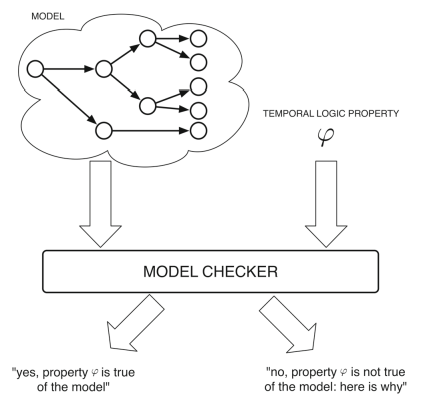
\includegraphics[width=0.75\linewidth]{chapters/checker_over.png}
%    \caption[Model Checking Overview]{Model Checking Overview~\cite{Abate2021}.}
%    \label{fig:modelchecking_flow}
%\end{figure}


%As presented in the picture, one has a set of requirements that need to be satisfied, usually given in a temporal logic (CTL, LTL), stating how the behavior of the systems evolves over time. One also needs to model the system under analysis in such a way that the model checking tool understands it, typically as a Transition System. 

%Once the transition system and temporal logic properties are defined, all that is needed is a model checker to assess whether the specified properties hold within the system.

%There are plenty of model checkers available and, the main difference between them is the algorithm (for optimization purposes). To start this project, some examples of other models Checkers will be described, but the main focus will be on \textbf{Imitator} and \textbf{Uppaal} because, as previously mentioned, it is in these two programs that the systems in Uppex will be shaped. 


\section{Model Checking real-time systems}

Model Checking is an automatic verification technique for finite state (concurrent) systems. Its a very important step in the development of a system to find errors and guarantee correct function \cite{Baier2008}. A summarized picture of the model checking process is given in Figure \ref{fig:modelchecking_flow}.


\begin{figure} [H]
    \centering
    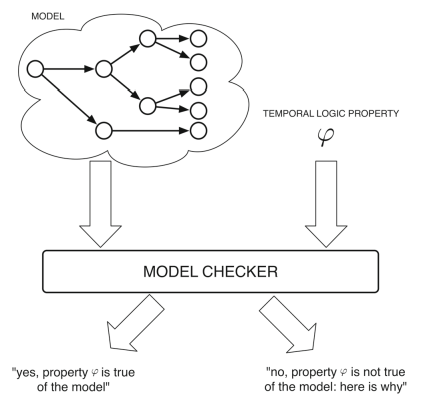
\includegraphics[width=0.75\linewidth]{chapters/checker_over.png}
    \caption[Model Checking Overview]{Model Checking Overview~\cite{Abate2021}.}
    \label{fig:modelchecking_flow}
\end{figure}


As presented in the picture, one has a set of requirements that need to be satisfied, usually given in a temporal logic (CTL, LTL), stating how the behavior of the systems evolves over time. One also needs to model the system under analysis in such a way that the model checking tool understands it, typically as a Transition System. 

%Once the transition system and temporal logic properties are defined, all that is needed is a model checker to assess whether the specified properties hold within the system.

There are many model checkers available, and what mainly distinguishes them is the algorithm they use, since each one adopts different optimization strategies, that is, they all solve the same verification problem but rely on different techniques(add here ref). To start this project, we present different examples of models checkers with\textbf{Imitator} and \textbf{Uppaal} on the spotlight as previously mentioned. It is within these two programs that the systems in Uppex will be modeled and analyzed.

\subsection*{SPIN}

 SPIN is an LTL model checker commonly used for modeling concurrent software and asynchronous processes, particularly communication protocols. It utilizes Promela as the modeling language. After we create our model, it offers the option to simulate the model randomly, interactively, or in a guided manner. Additionally, SPIN can create a C program that automatically performs exhaustive model checking ~\cite{spin}.

%In essence, the process involves the creation of a model system using Promela, which is then subjected to a verification by SPIN. SPIN can either simulate the model through various approaches or generate a C-based verifier. 
The verifier conducts exhaustive model checking, identifying violations of specified properties, such as safety and correctness. This methodology proves particularly valuable in scenarios where correctness and security are critical considerations, as is often the case in communication protocol applications (Figure~\ref{fig:Spin}).

\begin{figure} [H]
    \centering
    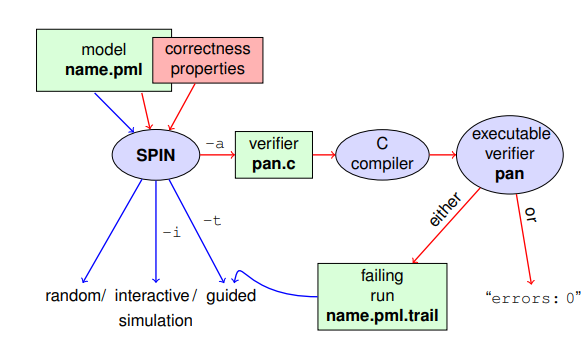
\includegraphics[width=0.75\linewidth]{chapters/spin.png}
    \caption[Spin Process]{Spin Process \cite{spin}.}
    \label{fig:Spin}
\end{figure}

\paragraph{}

\subsection*{Prism}

Prism is a Probabistic Model Checking tool that deals with systems that exhibit probabilistic behavior. Probabilistic model checking refers to a range of techniques for calculating the likelihood of the occurrence of certain events during the execution of systems ~\cite{prism}. As a input, Prism takes a probabilistic model, including \emph{Continuous-time Markov chains} and \emph{Probabilistic timed automata}, and a probabilistic temporal logic \cite{citacao6}. This is summarized in Figure~\ref{fig:prism}.

\begin{figure} [H]
    \centering
    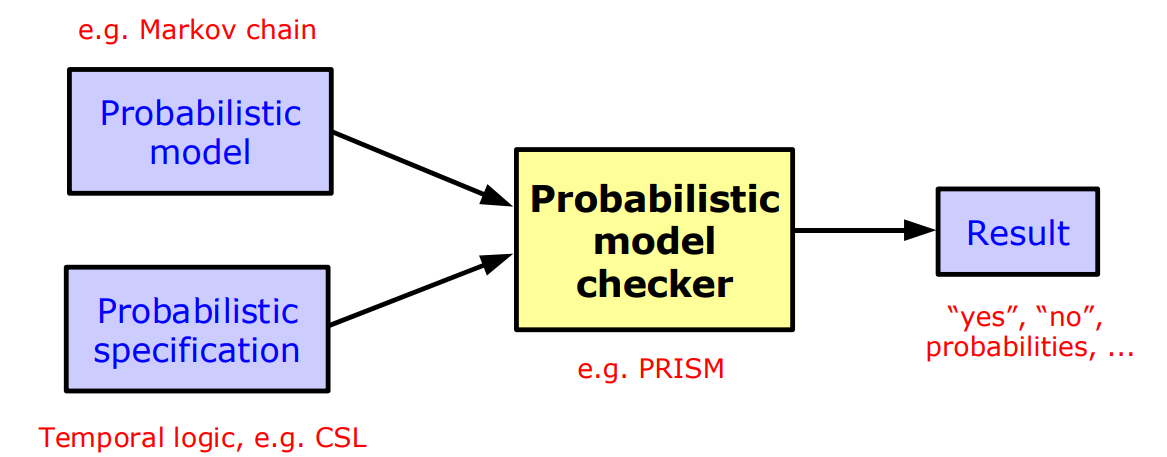
\includegraphics[width=0.9\linewidth]{chapters/Prism.png}
    \caption[Prism Process]{Prism Process~\cite{prism}.}
    \label{fig:prism}
\end{figure}

\paragraph{}

\subsection*{Simulink}

Simulink is a Matlab extension %which is a development and simulation language
that is widely used to \emph{model} and \emph{simulate} dynamical systems~\cite{Peled2001}. It is particularly suitable for specifying mathematical models of real time systems. Simulink has two different approaches to ensure that failures are identified as early as possible.

\begin{itemize}
    \item \textbf{Model testing} attempts to identify failures in models by executing them for some test inputs sampled by a guided randomized algorithm~\cite{Haque2022}.

    \item \textbf{Model checking} attempts to exhaustively verify the correctness of models against some given formal properties~\cite{Haque2022}.
\end{itemize}

In the case of Model checking, the inputs (system and property) are translated and used as inputs in some model checker or Satisfiability Modulo Theories (SMT) solvers. Since Simulink models often represent continuous dynamic and hybrid systems, applying model checking to such models typically leads to undecidable~\cite{Chakraborty2011}.

%colocar o uppaal e imitator

\section{Uppaal in a Nutshell}

As mentioned previously, Uppaal is a model checking tool for verification of real time systems jointly developed by Uppsala University and Aalborg University. In order to do that, Uppaal adopts the concept of Timed (Finite) Automata as model system (transistion system) \cite{Behrmann2006}. 

\subsubsection{Timed Automata}

A \textit{Timed Automaton} (TA) extends the concept of a Finite Automaton with clocks that are used to handle time in the system. Time is continuous and the clocks measure time progress which will increase globally at the same pace for the whole system. It is formally defined as a 6-tuple \cite{baier2008principles}:



\[
\langle L, L_0, Act, C, Tr, Inv \rangle
\]

Where:
\begin{itemize}
    \item \( L \) is the set of \textbf{locations} (or states).
    \item \( L_0 \subseteq L \) is the subset of \textbf{initial locations}.
    \item \( Act \) is the set of \textbf{actions}, and \( C \) is the set of \textbf{clocks}.
    %\item \( Tr \subseteq L \times \mathcal{C} \times Act \times \mathcal{P}(C) \times L \) defines the \textbf{transition relation}, i.e., the rules that determine how the system evolves.
\end{itemize}

Before defining transitions, it is crucial to introduce the concept of a reset. In a timed automaton, the value of a clock can be reset during transitions.

The power set \( P(C) \) represents all possible subsets of the clocks \( C \) that could be reset during a transition ~\cite{baukus2002power}. For example, if \( C = \{x, y\} \), then the power set of \( C \) is:

\[
P(C) = \{\emptyset, \{x\}, \{y\}, \{x, y\}\}
\]

This describes the four possible ways clocks can be reset:

\begin{itemize}
    \item \( \emptyset \): No clocks are reset.
    \item \( \{x\} \): Only clock \( x \) is reset.
    \item \( \{y\} \): Only clock \( y \) is reset.
    \item \( \{x, y\} \): Both clocks \( x \) and \( y \) are reset.
\end{itemize} 

The notation \( \mathcal{C}(C) \) denotes the set of clock constraints over a set \( C \) of clock variables. Each constraint is formed according to \cite{baier2008principles}:

\[
g ::= x \ \square \ n \mid x - y \ \square \ n \mid g \land g \mid \text{true}
\]
where \( x, y \in C \), \( n \in \mathbb{N} \), and \( \square \in \{ <, \leq, >, \geq, = \} \). These will be used in \textbf{guards} (on the transitions) or in \textbf{invariants} (on the locations). It is worth noting that invariants are the only way to enforce a transition \cite{baier2008principles}. 

We can also define the Invariant Function ($Inv$) as follows:

\begin{itemize}
    \item $Inv: L \rightarrow \mathcal{C}(C)$ is the \textbf{invariant function} that assigns a clock constraint to each location $\ell \in L$.
\end{itemize}

With this concepts in place, we can now complete the formal notation for transitions:

\begin{itemize}
    \item \( Tr \subseteq L \times \mathcal{C} \times Act \times \mathcal{P}(C) \times L \) defines the \textbf{transition relation}, i.e., the rules that determine how the system evolves.
\end{itemize}


The transition notation:
\[
\ell_1 \xrightarrow{g, a, U} \ell_2
\]

means that:
\begin{itemize}
    \item The system can transition from location \( \ell_1 \) to \( \ell_2 \) if the \textbf{guard} \( g \) is valid.
    \item The transition is labeled by an \textbf{action} \( a \).
    \item When the transition occurs, the \textbf{clocks} in set \( U \) are reseted.
\end{itemize}

%The power set \( P(C) \) represents all possible subsets of the clocks \( C \) that could be reset during a transition ~\cite{baukus2002power}. For example, if \( C = \{x, y\} \), then the power set of \( C \) is:

%\[
%P(C) = \{\emptyset, \{x\}, \{y\}, \{x, y\}\}
%\]

%This describes the four possible ways clocks can be reset:

%\begin{itemize}
%    \item \( \emptyset \): No clocks are reset.
%    \item \( \{x\} \): Only clock \( x \) is reset.
%    \item \( \{y\} \): Only clock \( y \) is reset.
%    \item \( \{x, y\} \): Both clocks \( x \) and \( y \) are reset.
%\end{itemize} 

%The notation \( \mathcal{C}(C) \) denotes the set of clock constraints over a set \( C \) of clock variables. Each constraint is formed according to \cite{baier2008principles}:

%\[
%g ::= x \ \square \ n \mid x - y \ \square \ n \mid g \land g \mid \text{true}
%\]
%where \( x, y \in C \), \( n \in \mathbb{N} \), and \( \square \in \{ <, \leq, >, \geq, = \} \). These will be used in \textbf{guards} (on the transitions) or in \textbf{invariants} (on the locations). It is worth noting that invariants are the only way to enforce a transition \cite{baier2008principles}. 


Timed Labelled Transition Systems (TLTS) models the execution of TA through labeled transition systems, incorporating so-called delay transitions to capture the passage of time.


A TLTS is a model that introduces two types of transitions \cite{baier2008principles}: 

\begin{itemize}
    \item \textbf{Ordinary transitions}: Associated with actions, denoted by:
    \[
        s \xrightarrow{a} s' \quad \text{where} \quad a \in \text{Act}.
    \]
    \item \textbf{Delay transitions}: Represent the passage of time, denoted by:
    \[
        s \xrightarrow{d} s' \quad \text{where} \quad d \in \mathbb{R}^+_0.
    \]
\end{itemize}

These transitions must obey certain constraints \cite{baier2008principles}:

\begin{itemize}
    \item \textbf{Time additivity}: If \( s \xrightarrow{d} s' \) and \( 0 \leq d' \leq d \), then there exist intermediate states \( s'' \) such that:
    \[
        s \xrightarrow{d'} s'' \xrightarrow{d - d'} s'.
    \]
    \item \textbf{Determinism of delays}: If \( s \xrightarrow{d} s' \) and \( s \xrightarrow{d} s'' \), then necessarily \( s' = s'' \).
\end{itemize}

In terms of semantics, each TA defines a TLTS \( T(TA) \) whose states are pairs of the form \cite{baier2008principles}:
\[
    \langle \text{location}, \text{clock valuation} \rangle.
\]

Transitions follow specific rules, and if a transition depends on a clock \( x \), it only occurs if the associated time constraint is valid. Time can advance as long as the current state still satisfies its constraints.

Clocks are valuation functions \( \eta: C \to \mathbb{R}^+_0 \), mapping each clock \( x \) to its current value. The main operations on clocks are \cite{baier2008principles}:

\begin{itemize}
    \item \textbf{Delay}: Increases the value of all clocks, defined by:
    \[
        (\eta + d)(x) = \eta(x) + d.
    \]
    \item \textbf{Reset}: Resets certain clocks, defined by:
    \[
        \eta[R](x) = 
        \begin{cases}
            0, & \text{if } x \in R, \\
            \eta(x), & \text{otherwise}.
        \end{cases}
    \]
\end{itemize}

More specifically the conversion of a Timed Automaton to a TLTS \( T(ta) = \langle S, S_0, N, T \rangle \) occurs as follows \cite{baier2008principles}:

\begin{itemize}
    \item \( S \) is the set of states;
    \item \( S_0 \) is the set of initial states;
    \item \( N \) is the set of transition labels, including actions and delays;
    \item \( T \) is the set of transitions, defined by:
    \[
        \langle l, \eta \rangle \xrightarrow{a} \langle l', \eta' \rangle \quad \text{if there is a valid transition in } Tr.
    \]
    The delay transition occurs as long as the state invariants are maintained.
\end{itemize}




\subsubsection*{Modelling in Uppaal}

%A system in Uppaal is modeled as a network of TA in parallel \cite{proenca-spreadsheet-2023}. Each automaton is composed by a set of a locations, transistions are used to 'travel' throw all locations and to control those it is possible to use guards, invariant and a synchronization, as we saw before

A system in Uppaal is formally modeled as a network of Timed Automata (TA) that operate in parallel through a composition approach \cite{proenca-spreadsheet-2023}. This network consists of multiple interacting TA processes, where each automaton contains locations (discrete states) and transitions that enable movement between these locations. The behavior is controlled through clock constraints expressed as guards on transitions and invariants on locations, which enforce timing requirements. Additionally, synchronization between different automata is achieved through complementary actions, allowing coordinated behavior across the parallel components \cite{Behrmann2006}. During a Transistion we can also update the value of a variable or clock a \cite{upp}.

%\begin{itemize}
%    \item \textbf{Guard} A guard is a condition applied to the variables and the clocks. If is the condition is True the transistion is enable, otherwise cannot occur~\cite{Behrmann2006}.

%    \item \textbf{Invariants} Invariants are conditions that must be True while the automaton is in a specific location~\cite{Behrmann2006}.

%    \item \textbf{Synchronization}  In Uppaal, synchronization is based on a handshaking mechanism. When two processes take a transition simultaneously, one transition is labeled with \texttt{a!} (send) and the other with \texttt{a?} (receive). In this setup, the exclamation mark ``\texttt{!}'' denotes the sending action that actively triggers the synchronization, while the question mark ``\texttt{?}'' represents the receiving action, which waits for the corresponding send event to occur.

%~\cite{Behrmann2006}.
%\end{itemize}

%During a Transistion we can also update the value of a variable or clock a \cite{upp}.
\paragraph{}

It is now possible to build a model using Uppaal. As an example, it will be built a Worker and Hammer system (\ref{fig:worker model}), as mentioned before.

\begin{figure} [H]
    \centering
    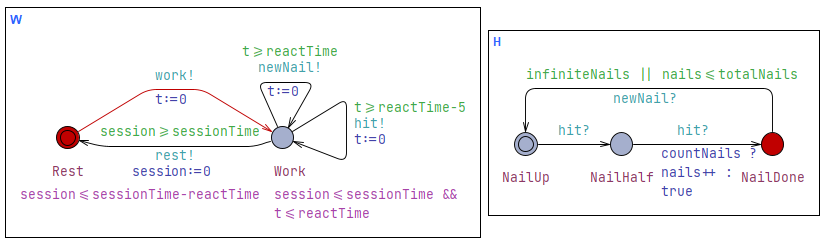
\includegraphics[width=\linewidth]{chapters/worker_hammer.png}
    \caption{Worker/Hammer Automata Example. The image on the left automaton represents the Worker, while the on on the right represents the Hammer.}
    \label{fig:worker model}
\end{figure}

%The worker automaton is made of two states as we see in Figure \ref{fig:worker model}: Rest (initial state) and Work. If the invariant condition is satisfied, a transistion to Work state is taken, synchronized with the event 'press!' and the clock t is restarted. 

%In state Work there are 3 possible transitions but one is excluded while the invariant of that state is satisfied. If t > reactTime,  newNail is done and the clock t is restarted. If t >reactTime -5 the synchronization hit is done and the hammer automata can finally start. When the invariant is no longer satisfied and the system satisfies the guard of the last transition, the automata goes back to the initial state, the clock session is restarted and the process can restart again.

%In Figure \ref{fig:worker model}, the right automaton, as mentioned, represents the Hammer. It has 3 states, none of which have invariants. The first transition occurs only when the "hit" synchronization is activated. The transition from "NailHalf" to "NailDone" happens after the "hit" is activated again, and during this process, the variable "countNails" is updated to a specific value. The last transition back to the initial state is only possible if the logical result of the conditions remains the same, and if the "newNail" synchronization is activated.

%To ensure the model's full functionality, it is essential to declare the variables used in the Uppaal model. The syntax used for declarations is very similar to the one used in C and can be defined as global or local.

%Its important to notice that sessionTime, ReactionTime, totalNails, TotalNail and CountNails are constants and not parameters. Uppaal can not support parameters in clocks, only in variables, if the user pretends to build a generic Process(Timed Automata). In this example sessionTime takes the value 100, ReactionTime 20, totalNails 10 and countNails and infineNails both True.

The Worker automaton consists of two states, as shown in Figure \ref{fig:worker model}: Rest (the initial state) and Work. When the invariant condition is satisfied, a transition to the Work state is triggered, synchronized with the event press!, and the clock t is reset.

In the Work state, there are three possible transitions, although one remains excluded as long as the state invariant holds. If t > reactTime, the transition newNail is executed and the clock t is restarted. If t > reactTime – 5, the synchronization hit is performed, enabling the Hammer automaton to start its execution. When the invariant of the state is no longer satisfied, and the guard of the final transition is met, the automaton returns to the initial state, the session clock is reset, and the process begins again.

In Figure \ref{fig:worker model}, the automaton on the right represents the Hammer. It is composed of three states, none of which contain invariants. The first transition occurs only when the hit synchronization is activated. The transition from NailHalf to NailDone takes place after a second activation of hit, during which the variable countNails is updated to a predefined value. The final transition, which returns the automaton to its initial state, is possible only if the logical conditions remain valid and the newNail synchronization is activated.

To ensure the complete functionality of the model, it is essential to declare the variables used in the Uppaal specification. The syntax for these declarations is very similar to that of C, and variables may be defined as either global or local.

It is important to note that sessionTime, reactionTime, totalNails, totalNail, and countNails are constants, not parameters. Uppaal does not support parameters in clocks, only in variables, when defining a generic process (Timed Automata). In this example, sessionTime is set to 100, reactionTime to 20, totalNails to 10, and both countNails and infiniteNails are set to True.


\subsubsection*{Verification in Uppaal}

The next phase is to check that the model verifies the properties and to do so, Uppaal also has a window dedicated to that (verification window). With Uppaal query language it can be specified the following properties (mentioned above):

\begin{itemize}
    \item \textbf{Reachability properties:} A specific condition that holds in some state of the model’s potential behaviours.

    \item \textbf{Safety properties:} A specific condition that holds in all the states of an execution path.

    \item \textbf{Liveness properties:} A specific condition is guaranteed to hold eventually.

    %\item \textbf{Deadlock properties:} A deadlock is possible or not in the model.
\end{itemize}

These properties can be described using a simple CTL logic variation (TCTL)\cite{lee2009timed}. It is a branching-time temporal logic used to formally specify and verify properties of systems, and it is based on the idea that all possible execution paths a system can take can be represented in the form of a "Computation Tree" \cite{lee2009timed}. The formulas should be one of the following \cite{bengtsson2004timed}:

\begin{itemize}
    \item A[] $\phi$ — Invariantly $\phi$

    \item E<> $\phi$ - Possibly $\phi$

    \item A<> $\phi$ - Always Eventually $\phi$

    \item E[] $\phi$ - Potentially Always $\phi$

    \item $\phi$ $\longrightarrow$ $\psi$ - $\phi$ leads to $\psi$
    
\end{itemize}

The symbols $\phi$ and $\psi$ are formulae that describe state properties, such as what is the current state and clock constrains. Returning to the worker and hammer example, we can illustrate some properties using this notation. Notice that Deadlock is expressed using a special formula and IT consists of the keyword deadlock. 

\begin{itemize}
    \item \textbf{A[]!deadlock} Deadlock never occurs.

    \item \textbf{A[] W.Rest} The Worker always reaches the Rest state.

    \item \textbf{E<> H.NailDone} The Hammer will eventually finish Nailing.

    \item  \textbf{A<> H.NailDone} The Hammer eventually reaches the NailDone state on all paths.

    \item \textbf{W.Work $\longrightarrow$ W.Rest} If the Worker is in the Work state, then it will eventually reach the Rest state.
\end{itemize}

%These properties can be verified on the Verifier, if the property is marked in red it means 'not satisfied' otherwise its satisfied.
These properties can be verified in the Verifier. The Verifier is a tool that checks if your model behaves as expected. If the property is marked in red, it means 'not satisfied' (the model does not guarantee the property). Otherwise, it is 'satisfied' (the model always meets the condition).

%\paragraph{}


%\textbf{Limitations}

%Uppaal is known for its intuitive nature and for being easy to lear, making it accessible even to users with limited knowledge of finite automata. It has a user-friendly interface which facilitates the process of building models, allowing users to create and manipulate designs in a easy way.

%Although its advantages, it has some limitations. For example:

%Uppaal may face limitations when it comes to describing true real-time systems, especially within the context of embedded systems. In many cases, real-time systems are components of larger embedded systems, and the values they receive from the overall system can be predetermined or pre-established.
%One of the challenges with Uppaal is its inability to fully support parameterized clocks and dynamic conditions that may be prevalent in complex real-time systems. Real-time systems often involve intricate interactions with external components, which may have varying inputs and conditions. Uppaal's current capabilities may not fully capture the dynamic and parameterized nature of these interactions, potentially limiting its effectiveness in modeling certain aspects of real-time embedded systems.
%Therefore, while Uppaal may be suitable for certain types of real-time systems, it may not provide the flexibility and expressiveness needed for more intricate embedded systems with dynamic conditions and parameterized clocks. Users may need to consider alternative tools or approaches that better accommodate the complexities of their specific real-time embedded systems.


\section{Imitator in a Nutshell}

IMITATOR is command-line only tool to perform automated parameter synthesis for parameter timed systems. This model checker takes as input a network of Parametric Timed Automata. This type is a sub category of timed automata where clocks can be declared as parameters (without a constant pre-determined), making it particularly useful for modeling \textbf{Real-Time Systems} and \textbf{Software Product Lines (SPLs)}~\cite{IMITATOR}. In real-time systems, timing constraints often depend on environmental conditions or system configurations. By allowing certain timing constraints to remain as parameters rather than fixed values, Parametric Timed Automata enable the analysis of multiple scenarios, ensuring that the system behaves correctly under various conditions \cite{RealTimeSystems}.
Similarly, in Software Product Lines (SPLs), where models need to be adapted and reused across different products or configurations, the use of parametric timing constraints avoids the need to create separate automata for each variation. A single model can be created where critical variables can be written as paramaters. This enhances flexibility and reduces redundancy in system modeling ~\cite{SPL}.


Imitator is a model checker specialized in analyzing parametric systems. Its strength lies not only in verifying whether system properties hold but also in determining the exact conditions (parameter constraints) under which they are satisfied. By using Imitator, we can systematically evaluate a model and check if the properties defined in the property.imiprop file are valid, while also obtaining the precise parameter values required for them to hold. Moreover, Imitator goes beyond mere verification by offering insights into the constraints under which these properties are valid. This information is valuable for understanding the system's behavior and can guide further refinement or optimization to enhance the system's reliability and performance~\cite{IMITATOR}.

\subsubsection{Parametric Timed Automata}

A \textit{Parametric Timed Automaton} (PTA) is a generalization of TA that introduces parameters in the guards and resets of clocks, allowing the modeling of systems where certain temporal values are unknown or variable. Unlike TA, where timing bounds are fixed, PTA enable symbolic analysis and the synthesis of constraints on these parameters. It is formally defined as a 7-tuple \cite{andrePTA}.



\[
\langle L, L_0, Act, C, Tr, \textcolor{red}{P}, Inv\rangle
\]

Where:
\begin{itemize}
    \item \( L \) is the set of \textbf{locations} (or states).
    \item \( L_0 \subseteq L \) is the subset of \textbf{initial locations}.
    \item \( Act \) is the set of \textbf{actions}, and \( C \) is the set of \textbf{clocks}.
    \item \textcolor{red}{\( P \text{ is a finite set of parameters.} \)}
    \item \( Tr \subseteq L \times \mathcal{C}(C) \times Act \times \mathcal{P}(C) \times L \) defines the \textbf{transition relation}, i.e., the rules that determine how the system evolves.
\end{itemize}

The transition notation:

\[
\ell_1 \xrightarrow{g, a, U} \ell_2
\]

Means that:
\begin{itemize}
    \item The system can transition from location \( \ell_1 \) to \( \ell_2 \).
    \item This transition occurs if the \textbf{guard} \( g \) is valid.
    \item The transition is labeled by an \textbf{action} \( a \).
    \item When the transition occurs, the set of \textbf{clocks} \( U \) is reset.
\end{itemize}

The power set \( P(C) \) represents all possible subsets of the clocks \( C \) that could be reset during a transition ~\cite{baukus2002power}. For example, if \( C = \{x, y\} \), then the power set of \( C \) is:

\[
P(C) = \{\emptyset, \{x\}, \{y\}, \{x, y\}\}
\]

This describes the four possible ways clocks can be reset:

\begin{itemize}
    \item \( \emptyset \): No clocks are reset.
    \item \( \{x\} \): Only clock \( x \) is reset.
    \item \( \{y\} \): Only clock \( y \) is reset.
    \item \( \{x, y\} \): Both clocks \( x \) and \( y \) are reset.
\end{itemize} 

The notation \( \mathcal{C}(C) \) denotes the set of clock constraints over a set \( C \) of clock variables. Each constraint is formed according to:

\[
g ::= x \ \square \ n \mid x - y \ \square \ n \mid g \land g \mid \text{true}
\]
where \( x, y \in C \), \( n \in \mathbb{N} \), and \( \square \in \{ <, \leq, >, \geq, = \} \). These will be used in \textbf{guards} (on the transitions) or in \textbf{invariants} (on the locations). It is worth noting that invariants are the only way to enforce a transition \cite{proenca_slides}.

Regarding the semantics of the automaton, we define a \emph{parameter valuation} $v$ as a function that assigns concrete (numerical) values to the parameters $p_1, p_2, \ldots, p_n$ in the automaton. The result of applying $v$ to a parametric timed automaton (PTA) $A$ is denoted by $v(A)$, which corresponds to a non-parametric timed automaton --- that is, all parameters are replaced with specific constant values.

Given a PTA $A = (\Sigma, L, l_0, X, P, I, E)$ and a parameter valuation $v$, the \emph{concrete semantics} of $v(A)$ is defined by a \emph{timed labelled transition system}, as in the case of TA.


A TLTS (Timed Labelled Transition System) introduces two types of transitions:

\begin{itemize}
    \item \textbf{Ordinary transitions}: Associated with actions, denoted by:
    \[
        s \xrightarrow{a} s' \quad \text{where} \quad a \in \text{Act}.
    \]
    \item \textbf{Delay transitions}: Represent the passage of time, denoted by:
    \[
        s \xrightarrow{d} s' \quad \text{where} \quad d \in \mathbb{R}^+_0.
    \]
\end{itemize}

These transitions must obey certain constraints:

\begin{itemize}
    \item \textbf{Time additivity}: If \( s \xrightarrow{d} s' \) and \( 0 \leq d' \leq d \), then there exist intermediate states \( s'' \) such that:
    \[
        s \xrightarrow{d'} s'' \xrightarrow{d - d'} s'.
    \]
    \item \textbf{Determinism of delays}: If \( s \xrightarrow{d} s' \) and \( s \xrightarrow{d} s'' \), then necessarily \( s' = s'' \).
\end{itemize}

In terms of semantics, each Timed Automaton (TA) defines a TLTS \( T(ta) \) whose states are pairs of the form:
\[
    \langle \text{location}, \text{clock valuation} \rangle.
\]

Transitions follow specific rules, and if a transition depends on a clock \( x \), it only occurs if the associated time constraint is valid. Time can advance as long as the current state still satisfies its constraints.

Clocks are valuation functions \( \eta: C \to \mathbb{R}^+_0 \), mapping each clock \( x \) to its current value. The main operations on clocks are:

\begin{itemize}
    \item \textbf{Delay}: Increases the value of all clocks, defined by:
    \[
        (\eta + d)(x) = \eta(x) + d.
    \]
    \item \textbf{Reset}: Resets certain clocks, defined by:
    \[
        \eta[R](x) = 
        \begin{cases}
            0, & \text{if } x \in R, \\
            \eta(x), & \text{otherwise}.
        \end{cases}
    \]
\end{itemize}

The conversion of a Timed Automaton (TA) to a TLTS \( T(ta) = \langle S, S_0, N, T \rangle \) occurs as follows:

\begin{itemize}
    \item \( S \) is the set of states;
    \item \( S_0 \) is the set of initial states;
    \item \( N \) is the set of transition labels, including actions and delays;
    \item \( T \) is the set of transitions, defined by:
    \[
        \langle l, \eta \rangle \xrightarrow{a} \langle l', \eta' \rangle \quad \text{if there is a valid transition in } Tr.
    \]
    The delay transition occurs as long as the state constraints are maintained.
\end{itemize}




\subsubsection{Limitations in Parametric Timed Automata}

Introducing parameters in real-time temporal logic can indeed lead to undecidability issues, notably when such parameters are unbounded. On top of this, the use of multi-rate automata together with linear constraints on clocks also leads to undecidability, as does the use of stopwatches \cite{Andre2021}. The addition of parameters, increases the complexity of the model checking of these systems, this complexity often results in undecidability, meaning that there is no general algorithm that can determine the validity of formulas within the logic. In fact, most interesting problems that are decidable in timed automata become undecidable in Parametric Timed Automata, including the ones below \cite{Andre2021}.


\begin{itemize}
    \item \textbf{EF-emptiness}

    Is the set of parameter valuations for which a given location \( l \) is reachable empty?

    %\textcolor{red}{undecidable}

    \item \textbf{EF-universitily}

    Do all parameters allow to reach a given location \( l \)?

    %\textcolor{red}{undecidable}

    \item \textbf{AF-emptiness}

    Is the set of parameter valuations for which all runs eventually reach a given location \( l \) empty?

    %\textcolor{red}{undecidable}

    \item \textbf{AF-universitily}

    Do all parameters allow to reach a given location \( l \) for all runs?

    %\textcolor{red}{undecidable}

    \item \textbf{Language and Trace Preservation}

    For a given set of timing parameters, are there other parameter values that yield the same sequence of discrete events?

    %\textcolor{red}{undecidable}
\end{itemize}
 

However, there are adaptations that can be applied to the automaton to ensure the decidability of certain problems. For example, reducing parameters, parametric clocks, and non-parametric clocks result in the decidability of the EF-emptiness problem(Parametric clocks are time variables in parametric timed automata whose behavior depends on parameters that are unknown or undefined a priori) \cite{andre2019whats}. Another approach is through the restriction of parameter usage, utilizing a subcategory of Parametric Timed Automata called Lower/Upper Bound Parametric Timed Automata (L/U PTA), where all parameters are compared with the clocks either as an upper bound or a lower bound. With this restriction, several verification problems that are generally undecidable for general PTA become decidable \cite{andre2019whats}. In particular, the EF-emptiness problem (determining whether there exists an instantiation of parameters such that a given state is reachable), the EF-universality problem (checking whether all possible parameter valuations allow the reachability of a given state), and the EF-finiteness problem (determining whether the number of parameter valuations leading to reachability is finite) become decidable. These problems, which are crucial for analyzing the behavior of parametric timed systems, fall within PSPACE complexity when restricted to L/U PTA, ensuring their computational feasibility \cite{andre2019whats}. However, not all verification problems benefit from this restriction. Certain problems remain undecidable even under general PTA constraints. For instance, the AF-emptiness problem (determining whether there exists a parameter valuation such that all runs eventually reach a given state) is undecidable. Similarly, language preservation, which checks whether the language of a PTA remains unchanged under all possible parameter valuations, is also undecidable. Additionally, the EG-emptiness problem (verifying whether there exists a parameter valuation such that some execution remains within a given set of states indefinitely) remains an open question \cite{andre2019whats}.


%Despite these undecidability results, the L/U PTA framework plays a crucial role in retaining decidability for many verification problems, providing a balance between expressiveness and computational feasibility. By ensuring that fundamental reachability and verification tasks remain within PSPACE complexity, L/U PTA continues to be a valuable tool for analyzing real-time systems in fields such as embedded systems, network protocols, and real-time control applications.


%\subsubsection*{Modelling in Imitator}

%The Imitator tool follows the same syntax logic as HyTech and can always be divided into three main parts.

%\begin{itemize}
%    \item \textbf{Variable declarations}

%    In the variable declaration block, we define the essential elements of the model, including constants, parameters, clocks, and state variables. These elements are used to represent temporal constraints and rules within the modeled system.

%    The clocks all evolve at the same rate of 1 time unit, and the way to declare them is with the suffix \textbf{: clocks} after defining their names.

%    Variables can be global or discrete (a name derived from the HYTECH tool syntax). Both are shared by all automata in the model, and unlike discrete variables, the value of global variables cannot be altered. Within discrete variables, there are several types, such as: Integers (Int), Booleans, Arrays, Lists, Stacks, and Queues. Just like with clocks, to declare these variables, you simply use the suffix \textbf{: Type}, where 'Type' represents the desired type from the ones mentioned earlier. 

%    \item \textbf{Automata}

%    In the Automata block, we define the timed automata that represent the system's behavior. It includes states, which represent different phases of the system, and transitions, which define how the system moves from one state to another. Additionally, it contains invariants, which impose constraints on the time that can be spent in a state, guards, which set conditions for a transition to occur, and assignments, which update variables or clocks after a transition.

%    Each location of the automaton is initialized with \textbf{loc}, followed by its name and, if present, an invariant. The definition continues with \textbf{when}, followed by the transition condition, \textbf{sync} for the synchronization action, \textbf{do} for variable or clock updates, and \textbf{goto} to indicate the next state. If there are multiple transitions from the same location, they are listed sequentially.

%    Each location can be urgent if no time passage is allowed in that location, defined by the keyword \textbf{urgent}. This means the system must leave this location immediately without allowing time to elapse. A location can be accepting if it represents a significant final state for verifying liveness properties. Accepting locations are used to define states that must be reached repeatedly in infinite executions, making them useful for checking the recurrence of desired behaviors. It is defined by the keyword \textbf{acepting}.
%    Additionally, a location can combine both properties, being both urgent and accepting, ensuring that the system reaches this location without delay and that it is considered for acceptance conditions in liveness verification.

%    It is also worth noting that the keyword \textbf{Stop} allows certain clocks to be interrupted in specific locations, while \textbf{Flow} enables the modification of the clock's evolution rate.

    
%    \item \textbf{Initial state definition}

%    The initial state definition section is split between the discrete initialization and the continuous initialization.
%    The discrete initialization (introduced by the discrete keyword) assigns an initial value to each discrete (global) variable, and sets the initial location for each automaton.
     %The continuous initialization (introduced by the continuous keyword) defines the initial constraints over clocks and parameters (possibly also using discrete variables).
%\end{itemize}

\definecolor{codebg}{rgb}{0.95,0.95,0.95}
\lstdefinestyle{imitator}{
    backgroundcolor=\color{codebg},
    basicstyle=\ttfamily\small,
    keywordstyle=\color{blue}\bfseries,
    commentstyle=\color{gray}\itshape,
    breaklines=true,
    frame=single,
    keepspaces=true,
    tabsize=4,
    showspaces=false,
    showstringspaces=false
}

%\begin{lstlisting}[style=imitator, caption=Variable Declarations Block]
%var
%    session, t
%    : clock;

%(*@Limits*)
%    sessionTime,
%    reactTime
%    : parameter;
%    nails
%    : discrete;
%    totalNails = 20
%    : constant;
%    b = True,
%    : bool;
%\end{lstlisting}


%\paragraph{}

%\begin{lstlisting}[style=imitator, caption=Automaton Worker]
%(*system*)
%automaton Worker

%synclabs: rest, hit, newNail, Work;

%loc Rest: invariant session <= sessionTime - reactTime
%    when True sync Work do {t := 0} goto Work;

%loc Work: invariant session <= sessionTime && t <= reactTime
%    when t >= reactTime sync newNail do {t := 0} goto Work;
%    when t >= reactTime - 5 sync hit do {t := 0} goto Work;
%    when session >= sessionTime sync rest do {session := 0} goto Rest;

%end
%\end{lstlisting}


%\begin{lstlisting}[style=imitator, caption=Automaton Hammer]
%automaton Hammer

%synclabs: hit, newNail;

%loc NailUp: invariant True
%    when True sync hit goto NailHalf;

%loc NailHalf: invariant True
%    when True sync hit do {nails := nails +1} goto NailDone;

%loc NailDone: invariant True
%    when nails <= totalNails sync newNail goto NailUp;

%end
%\end{lstlisting}


%\paragraph{}


%\begin{lstlisting}[style=imitator, caption=Initial state definition]
%(*system_enc*)
%init := 
%    & loc[Worker] = Rest
%    & loc[Hammer] = NailUp
%    & session = 0
%    & t = 0
%(*@limits2*)
%    & nails = 0
%    & sessionTime >= 0
%    & reactTime >= 0
%    & True;
%end
%\end{lstlisting}



%\paragraph{}


%To check if the system is syntactically correct and in the desired format, we save the code in a file with the .imi extension (e.g., system.imi). Then, we execute the following command in the terminal: \texttt{./imitator system.imi [property.imiprop] [-option]}

 

%The system.imi file serves as a model, representing systems such as the Worker and Hammer system. Alongside, the property.imiprop file contains all the properties that we aim to check. The -option in the command line allows to specify the desired output file format, whether it be PNG, Uppaal, or any other preferred format. It's important to note that the parameters enclosed in square brackets [] are optional~\cite{IMITATOR}.

\subsubsection*{Verification in Imitator}

To synthesize the system's parameters that validate the intended property based on the desired properties, Imitator offers two approaches to the parameter synthetise\cite{IMITATOR}:

\begin{itemize}
    \item \textbf{Synthesis (Synth)}

    IMITATOR attempts to synthesize all parameter valuations satisfying the property.

    \item \textbf{Witness}

    IMITATOR attempts to exhibit at least one parameter valuation satisfying the property.It works like syntesis but stops the analysis as soon as one such set is found
    
\end{itemize}

IMITATOR follows the "Best Effort" paradigm, meaning that attempts to synthesize a set of parameter valuations without guaranteeing termination, due to the undecidable nature of most problems in parametric timed automata. To ensure that the computation eventually halts, the tool relies on approximations, which often results in outcomes that are not sound or complete, meaning the results may include some incorrect parameter values (not sound) or miss some valid ones (not complete). The tool classifies its results into three categories and informs the user about them \cite{imitator_slides}.

\begin{itemize}
    \item \textbf{Exact}

    The synthesis found all and only the correct valuations.

    \item \textbf{Over-approximated}

    The set may contain invalid solutions.

    \item \textbf{Under-approximated}

    Some correct solutions may be missing.

    \item \textbf{Possibly invalid}

    There are no guarantees that the solution is correct.


\end{itemize}

In terms of properties, IMITATOR supports a vast number of properties, including reachability (“EF”), safety (“AG not”), liveness, deadlock-freeness and trace preservation (robustness). Additionally, other algorithms will be discussed in the following chapters, such as Minimum-Time Reachability, which aims to synthesize parameter valuations that minimize the time required to reach a given state, and Optimal Parameter Reachability, which determines the minimum or maximum value of a parameter when reaching a specific state \cite{IMITATOR}. A summary of these properties and their corresponding syntax can be found in Table~\ref{tab:imitator-properties}.
%For example, considering the previous case, we can all synthesize parameter valuations for which the state NailDone in the Hammer automaton is reached at least once using the following query:


%\begin{verbatim}
% #synth EF(loc[Hammer] = NailDone)   
%\end{verbatim}


The result is displayed in the terminal as a printout, showing the constraint applied to the parameters if they exist in the model. Otherwise, the output will be "True" or "False." Additionally, the result can be complemented with a graphical visualization, which can be requested at the end of the command using the options parameter as mentioned above. We will see this applied to examples in the next chapter.


\begin{table}[H]
\centering
\caption{Some Properties and their correspondence syntax in IMITATOR \cite{IMITATOR}}
\label{tab:imitator-properties}
\begin{tabular}{|c|c|}
\hline
\textbf{Property} & \textbf{Syntax Examples} \\ \hline
Deadlock Free & property := synth DeadlockFree ; \\ \hline
Safety & property := synth AGnot(State Predicate); \\ \hline
Reachability & property := synth EF(State Predicate); \\ \hline
Optimal parameter reachability & property := synth EFpmin/pmax(State Predicate,Parameter); %\footnote{Parameter that we want to minimize or maximize}
\\ \hline
Liveness & property := synth CycleThrough(State Predicate); \\ \hline
Robustness & property := synth TracePreservation(Parameters); \\ \hline
\end{tabular}
\end{table}

Other interesting properties are:

\begin{itemize}
    \item \textbf{Inverse Method} 

    \item \textbf{Behavioral cartography} 

    \item \textbf{Minimal-time reachability}

    %Lowest parameter constrain in order to reach certain state in the lowest time~\cite{imi}

\end{itemize}

It is important to note that the CycleThrough algorithm does not cover all Liveness properties. It only verifies whether there exists a cycle in the system (infinitely executable) that visits a given location infinitely often—that is, it ensures that a certain state will eventually be visited and will continue to be visited over time. More complex properties, such as verifying that whenever A occurs, eventually B occurs, or that all executions eventually reach a state X, must be verified using a different algorithm written under the observer formalism \cite{IMITATOR}.

An observer is a parametric timed automaton placed in parallel with the system (usually referred to as the Test Automaton) that neither alters nor constrains its behavior, acting instead as a trigger when a given property is violated. This approach allows more complex properties, such as Safety or Liveness, to be reduced to a Reachability property \cite{observers}.


The synthesis process generates a text file containing a detailed description of the system, along with computational information related to the synthesis, including the type of approximation performed. The key result of interest, the parameter constraint, is located in the section marked by \texttt{BEGIN CONSTRAINT} and \texttt{END CONSTRAINT}. An example of this file can be found in \texttt{Appendix B}, with the mentioned section clearly identified.


\section{Uppex in a Nutshell}

Uppex is a tool that facilitates the creation of a family of software product lines using a list of features defined in an Excel spreadsheet~\cite{uppex}. The process begins by defining configurations, where each configuration represents a unique combination of features. Features correspond to system characteristics, such as "slow" or "fast". Not all feature combinations are valid, some may be semantically inconsistent. To prevent such invalid combinations, Uppex uses a separate sheet where features are organized in a tree-like structure. In this structure, features located on the same leaf cannot be selected simultaneously, ensuring that only meaningful configurations are generated. Additionally, a Limits and Queries sheet is maintained, in which queries are defined through formulas and constants are assigned predefined values according to the configuration being executed. To execute, it is necessary to ensure that both the JVM and Uppaal are installed. Once verified, the latest .jar file can be used to run the command uppex runAll model.xml.

\subsection*{Overview of Software product lines}

We can define a
A software product line (SPL) %as a set of methods used to create similar/generic systems, called variants, from a set of systems that share a set of Features~\cite{Pohl2018}.%\cite{spl,spl2}.
as a technique to describe and develop a family of software products with many common artefacts, which are called \emph{features}. 
Each valid combination of features describes a possible software product from this SPL.
This techniques have been used by many companies, facilitating the development, analysis, and deployment of several large software artefacts with commonalities~\cite{Pohl2018}.
% With this, companies that implement the systems save time and money in production and focus on other developments~\cite{Pohl2018}.
%
There are many ways to implement SPL, which can be grouped %most of them
into two groups~\cite{Pohl2018}:

\begin{itemize}
    \item \textbf{Compositional Approaches}
    \item \textbf{Annotative Approaches}
\end{itemize}

In Compositional Approaches, features are treated as separate systems or code fragments that extend the base code. The key idea is to compose them in parallel. After defining certain features, they are integrated into the system. This integration can be done in different ways, ranging from simple concatenation to complex code transformations. Among the various types of parallel composition, the most notable are: \textbf{feature-oriented programming}, \textbf{aspect-oriented programming}, and \textbf{delta-oriented programming}.

In the other hand we have Annotative Approaches where annotations or markings are used to control the presence or absence of the Features that we want to add to the system (in this case they are already present in the base code). For example, in C and C++ programming languages, preprocessor directives such as ifdef, ifndef, else, and endif are used to conditionally include or exclude blocks of code during compilation.


\subsection*{Overview of Uppex}

Uppex is a tool developed in Scala that uses Apache POI libraries to read Microsoft documents. Its main goal is to simplify the construction and verification of multiple Uppaal models generated from different configurations of a single file, following the principles of Software Product Lines previously studied. The tool relies on an annotation mechanism to allow customization of various parts of the model, such as channels, shared variables, data types, time bounds, and requirements.

Uppex reads an Excel file containing the configurations and a Uppaal file with the source model with annotations, and generates a new Uppaal file for each configuration found. Each generated file replaces the original model and is verified by Uppaal. The output is an HTML report summarizing the generated configurations and the properties that were verified. The workflow follows the structure illustrated in Figure \ref{fig:Uppex WorkFlow}.

\begin{figure} [H]
    \centering
    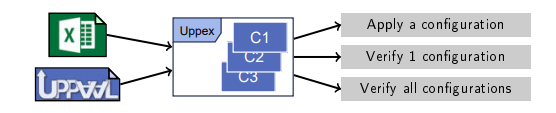
\includegraphics[width=\linewidth]{images/uppex_flow.png}
    \caption{Uppex WorkFlow \cite{proenca_uppex}}
    \label{fig:Uppex WorkFlow}
\end{figure}

The declarations that indicate annotations in the Uppaal file follow the format \textit{"// @Name"} and continue until a blank line is encountered. These serve as hooks that allow Uppex to inject and update the values used to configure the model, and are referred to simply as annotations. To inject and update the queries to be verified for each configuration, a different annotation is used, called a XML annotation. As the name suggests, it encompasses blocks that start with \textit{"<Name>"} and end with \textit{"</Name>"}. Each of these annotations is defined in the Excel file on a sheet with the same name. The first cell of the sheet specifies the pattern to be followed in order to generate the code that will be injected into the annotation block with the corresponding name in the Uppaal file. This is followed by a table where one column contains the name of the variable to be inserted, and the next columns specify the type and value of the variable separately. Additionally, there is a column named Feature that indicates which variables are active in the current configuration, discarding the others. In cases where duplicate variable names exist, only the last occurrence is considered. The configuration declarations are defined in the "@Configurations" sheet, with each configuration representing a combination of the existing features.To control the valid combinations of features, there is another sheet named "@FeatureModel", where the features are organized in a tree structure. In this structure, features that share the same root node cannot be selected simultaneously.

\subsection*{Revisiting the Worker and Hammer example}

%To better understand how it works, we can use the Worker and Hammer system as an example.
We will use the Worker and Hammer system to illustrate our description.


%Model Checking real time systems is a complex task because of nondeterminism and large number of states, which quickly leads to an explosion of states.

%One of the ways to combat this problem is to use the Uppex tool. Its a command only tool with a Excel file as frontend. From a generic model of a system and with Features selected by the user supports the creation and verification of variations of this model. Variations with fewer states and simpler. Another advantage of the tool is that the interaction between the user and the tool is through an excel file which reduces interaction with the Checker model~\cite{uppex,uppex-railway}. The model checker used by Uppex is Uppaal.


\begin{figure} [H]
    \centering
    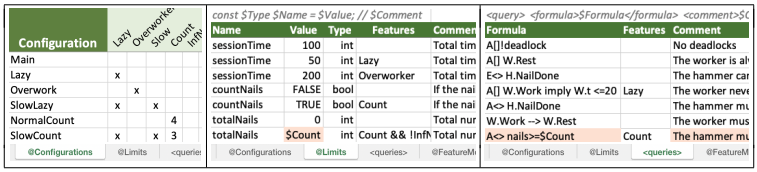
\includegraphics[width=\linewidth]{chapters/uppex.png}
    \caption{Uppex Configuration, Limits and Queries Sheets}
    \label{fig:WH_uppex}
\end{figure}

\begin{figure} [H]
    \centering
    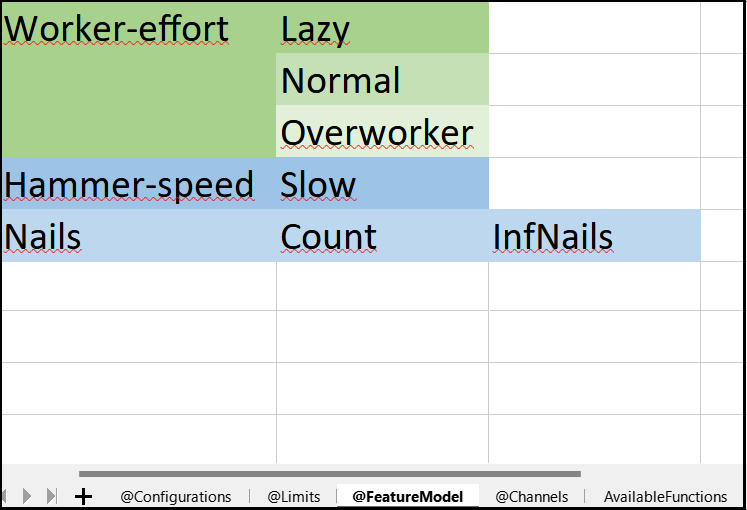
\includegraphics[width=0.4\linewidth]{images/upe_WH.png}
    \caption{Uppex Feature Model Sheet}
    \label{fig:WH_FM}
\end{figure}

Figure \ref{fig:WH_uppex} represents the Configurations, Limits, and Querie sheets, respectively. Assuming Lazy is the active configuration, the annotation block is rewritten using the following pattern:\texttt{const \$Type \$Name = \$Value; //\$Comment}, where the \texttt{\$} notation identifies the column from which the value should be extracted and replaced. Furthermore, as previously explained, only the values whose Feature matches the selected configuration (in this case, Lazy) are left blank will be considered.
\paragraph{}

%% usar fonte do codigo imitator

\begin{figure}[H]
\centering
\begin{minipage}{2.9\linewidth}
\begin{lstlisting}[language=MOREUPPAAL]
// @Limits
const int sessionTime = 50; // Total time that the worker can work
                            // before stopping 
const bool countNails = false; // If the nails should be counted. 
// If so, the system will have an infinite amount of states. 
const int totalNails = 0; // Total number of new nails available
                          // (when counting nails) 
const bool infiniteNails = false; // If there is no bound on the
                          // number of nails (can cause overflows) 
const int reactTime = 20; // Maximum time that the worker can take to
                          // hit or place a new nail 
\end{lstlisting}
\end{minipage}
\caption{Limits Block Rewritten with new values}
\label{fig:worker-config}
\end{figure}

The ``<queries>'' sheet follows the same logic, but it refers to a XML annotation, using the following pattern: \texttt{\footnotesize const \$Type \$Name = \$Value; // \$Comment}

\begin{figure}[H]
\centering
\begin{minipage}{0.9\linewidth}
{\footnotesize
\begin{verbatim}
    <queries>
    <query>
      <formula>A[]!deadlock</formula>
      <comment>No deadlocks</comment>
    </query>
    <query>
      <formula>A[] W.Rest</formula>
      <comment>The worker is always resting</comment>
    </query>
    <query>
      <formula>E&lt;&gt; H.NailDone</formula>
      <comment>The hammer can finish a nail</comment>
    </query>
    <query>
      <formula>A&lt;&gt; H.NailDone</formula>
      <comment>The hammer must complete a nail</comment>
    </query>
    <query>
      <formula>W.Work --&gt; W.Rest</formula>
      <comment>The worker must be able to rest after working</comment>
    </query>
    </queries>
\end{verbatim}
}
\end{minipage}
\caption{Queries Block Rewritten with new values}
\label{fig:worker-config}
\end{figure}

It is also important to highlight the constraints on feature combinations illustrated in Figure \ref{fig:WH_FM}. For instance, the user cannot select both Lazy and Overworker in the same configuration, thus preventing illogical or inconsistent combinations. Once the Excel configuration is complete, Uppex can be executed. The tool is distributed as a .jar file, which means it can be run directly from the command line. Uppex offers several execution options, allowing for flexible use depending on the user's needs. For example, it is possible to:

\begin{itemize}
    \item Run a specific configuration only (e.g., run the configuration named Main);

    \texttt{java -jar uppex.jar --run -p Main Model.xml}

    \item Validate the model and input files before generating the Uppaal models;
    
    \texttt{java -jar uppex.jar --validate Model.xml}
    
    \item Run all configurations defined in the Excel file, generating one Uppaal model for each and verifying the corresponding properties;
    
    \texttt{java -jar uppex.jar --runAll Model.xml}
\end{itemize}

As an example, we will choose the last option and run all configurations. When executed, Uppex generates an HTML report as output, summarizing the models and properties analyzed for each configuration. For the previous example, the resulting report can be found in the attachment.


%Sheet Configurations is responsible for variations of the Hammer and Worker file in uppaal. If we recall the worker and hammer example in the 'Uppaal in a Nutshell' section we had declared the variables sessionTime,countNails,totalNails,infiniteNails and reactTime and we had given a value to show how the tool works. It turns out that the Uppex tool takes these variables and depending on the settings they receive certain values. For example if we select Lazy, the sessionTime variable takes the value 200. The same happens with queries, are also checked according to the settings of the first sheet~\cite{uppex}.



%\section{The problem and its challenges}

%The next steps will consist of a first phase in the Imitator Connection with the Uppex Tool ensuring that it meets the same features that were already guaranteed by Uppaal. In a second resort take advantage of the capabilities of parameter synthesis (something that as we mentioned is not allowed in Uppaal) and apply these to Uppex.

%The next steps will consist of two main phases aimed at integrating and extending the capabilities of the Uppex tool. In the first phase, the focus will be on establishing a connection between Uppex and Imitator, ensuring that the tool can replicate the same functionalities and behavioral guarantees that were previously achieved through Uppaal. This includes verifying that the model configurations generated by Uppex remain valid and correctly verifiable when passed to Imitator, especially regarding the timing constraints, synchronization channels, and logical properties. The goal is to maintain functional parity with Uppaal while enabling compatibility with Imitator's framework.

%In the second phase, the aim is to leverage Imitator’s powerful capabilities for parameter synthesis—a feature that, as previously discussed, is not supported by Uppaal. By integrating parameter synthesis into the Uppex workflow, it becomes possible to not only verify specific configurations but also explore ranges of parameter values for which certain properties hold. This enhancement would allow the tool to support more advanced forms of design-space exploration, robustness analysis, and automated configuration tuning, significantly expanding the potential use cases of Uppex beyond traditional model checking.

%Ultimately, this extension will enable Uppex to support a broader class of problems and contribute to the development of more flexible and intelligent verification workflows in systems modeled with timed automata.

\section{Proposed extensions to Uppex}

%%colocar as secções deste capitulo

With the Imitator Model Checker and the Uppex tool introduced, the following chapters will detail the integration of Imitator into Uppex's backend as an alternative Model Checker to Uppaal. This integration also brought improvements to the types of supported features, the range of accepted properties and models, as well as enhancements to the final report generated by Uppex. Additionally, the first steps were taken toward developing a graphical user interface for the tool, aiming to provide a more user-friendly experience and reduce reliance on the terminal.



%como e que a nossa contribuição se relaciona com o que ja existe

% !TeX root = ../dissertation.tex

\chapter{Modelling in Imitator}


To explore the capabilities of the Imitator tool in greater detail, we begin by thoroughly defining its syntax, outlining the process of building a complete model in Imitator (Section~\ref{sec:specifying_automata}). The rest of this chapter describes how to use Imitator using four real-time systems (Section~\ref{sec:examples}): a \emph{Traffic Light System}, a \emph{Coffee Machine}, a \emph{Worker Hammer System} and a simple \emph{ATM Machine}. For each system, parameter synthesis will be demonstrated by verifying parameter constraints to prevent deadlocks. Additionally, one of the parameters in each system will be optimized.

\section{Specifying automata}\label{sec:specifying_automata}

The Imitator tool can always be divided into three main parts. In each part, the worker automaton from the worker and hammer example presented in Chapter 2 will be used to illustrate the Imitator's syntax.

\newcommand{\kw}[1]{\texttt{\textbf{\textcolor{blue!80!black}{#1}}}}

\begin{itemize}
    \item \textbf{Variable declarations}

    % \begin{figure}[H]
    % \centering
    \begin{lstlisting}[language=UPPAAL, caption={Variable Declaration Exemple using Worker Automata}, label={lst:VD_example_1}, float={bt}]
    var   session, t             : clock;
          sessionTime, reactTime : parameter;   
    \end{lstlisting}
    % \end{figure}

    In the variable declaration block, illustrated in Listing~\ref{lst:VD_example_1},
    we define the essential elements of the model, including \kw{clock}s, discrete variables, \kw{constant}s, and \kw{parameter}s. These elements are used in expressions that represent temporal constraints in the rest of the model.

    The \kw{clock}s are special variables that can evolve continuously, all at the same rate.
    % and the way to declare them is with the suffix \textbf{: clocks} after defining their names.
    Traditional variables are discrete and have an assigned type, which can be \kw{Int} (integer), \kw{Boolean}, \kw{Array}, etc., written e.g. \texttt{x : \kw{Int}} for an integer variable. Only discrete variables can be shared among different automata. Variables marked with \kw{constant} cannot be modified.
    Finally, a \kw{parameter} is an undefined variable that is inferred automatically by Imitator, which will be explained later.

    % Both are shared by all automata in the model and, unlike discrete variables, the value of global ones cannot be altered. Within discrete variables, there are several types, such as: Integers (Int), Booleans, Arrays, Lists, Stacks, and Queues. Just like with clocks, to declare these variables, you simply use the suffix \textbf{: Type}, where 'Type' represents the desired type from the ones mentioned earlier.

    % We can see an example of the variable declaration in Listing \ref{lst:VD_example}.



    \item \textbf{Automata}

    In the Automata block, we define the timed automata that represent the system's behavior. It includes states, which represent different phases of the system, and transitions, which define how the system moves from one state to another. Additionally, it contains invariants, which impose constraints on the time that can be spent in a state, guards, which set conditions for a transition to occur, and assignments, which update variables or clocks after a transition.

    Before constructing the automaton, it is necessary to explicitly declare all the synchronization actions present in the model using the keyword \kw{synclabs}, followed by the corresponding transitions.

    Each location of the automaton is initialized with \kw{loc}, followed by its name and, if present, an invariant. The definition continues with \kw{when}, followed by the transition condition, \kw{sync} for the synchronization action, \kw{do} for variable or clock updates, and \kw{goto} to indicate the next state. If there are multiple transitions from the same location, they are listed sequentially.

    Each location can be urgent if no time passage is allowed in that location, defined by the keyword \kw{urgent}. This means the system must leave this location immediately without allowing time to elapse. A location can be accepting if it represents a significant final state for verifying liveness properties. Accepting locations are used to define states that must be reached repeatedly in infinite executions, making them useful for checking the recurrence of desired behaviors. It is defined by the keyword \kw{acepting}.
    Additionally, a location can combine both properties, being both urgent and accepting, ensuring that the system reaches this location without delay and that it is considered for acceptance conditions in liveness verification.

    It is also worth noting that the keyword \kw{Stop} allows certain clocks to be interrupted in specific locations, while \kw{Flow} enables the modification of the clock's evolution rate.

    

    \begin{figure}[H]
    \centering
    \begin{lstlisting}[language=UPPAAL, caption={Construction of the Automata using Worker Automata as Example}, label={lst:VD_example}]
    (*Worker Automata*)
    automaton Worker
    
    synclabs: rest, hit, newNail, Work;
    
    loc Rest: invariant session <= sessionTime - reactTime
      	when True sync Work do {t := 0} goto Work;
    
    loc Work: invariant session <= sessionTime && t <= reactTime
      	when t >= reactTime sync newNail do {t := 0} goto Work;
      	when t >= reactTime - 5 sync hit do {t := 0} goto Work;
      	when session >= sessionTime sync rest do {session := 0} goto Rest;
    
    end	(* Worker *)
    \end{lstlisting}
    \end{figure}

    

    
    \item \textbf{Initial state definition}

    The initial state definition section is split between the discrete initialization and the continuous initialization. This section starts with the keyword \kw{init}, with each condition separated by \kw{\&}.
    The discrete initialization (optional introduced by the discrete keyword) assigns an initial value to each discrete variable, and sets the initial location for each automaton.
     The continuous initialization (optional introduced by the continuous keyword) defines the initial constraints over clocks and parameters (possibly also using discrete variables).

    \begin{figure}[H]
    \centering
    \begin{lstlisting}[language=UPPAAL, caption={Initial state definition using Worker Automata as Exemple}, label={lst:VD_example}]
    init := loc[Worker] = Rest
          & session = 0
          & t = 0
          & sessionTime >= 0
          & reactTime >= 0;
    end (* of file *)
    \end{lstlisting}
    \end{figure}
    
\end{itemize}
% \paragraph{}

\section{Specifying queries}
%explicar ficheiro separado e exemplificar prop anteriores


Finally, in terms of the syntax of the queries, which, as explained earlier, are written in a separate file, the query consists of the synthesis mode (synth or witness) and the synthesis algorithm. This condition is known as a state predicate that defines a specific state of an automaton. It typically takes the form loc[AUTOMATON] = LOCATION, where AUTOMATON is the name of the automaton and LOCATION is the name of a location within it. State predicates support logical operations like conjunction (AND), disjunction (OR), and can also involve global discrete variables \cite{IMITATOR}. The query is stored in a separate file with the \texttt{.imiprop} extension.

To check if the system is syntactically correct and in the desired format, we save the code in a file with the .imi extension (e.g., system.imi). Then, we execute the following command in the terminal: \texttt{./imitator system.imi [hammer\_proprities.imiprop]}. The system.imi file serves as a model, representing various systems. Alongside, the property.imiprop file contains all the properties that we aim to check. The -option flag in the command line allows to specify the desired output file format, whether it be PNG, Uppaal, or any other preferred format. It's important to note that the parameters enclosed in square brackets are optional~\cite{IMITATOR}.

\section{Installing Imitator}
The easiest and fastest way to install Imitator is by using Docker. Other alternatives can be found online at \url{https://www.imitator.fr/}. You can download the Imitator docker image with the following command: \texttt{docker pull imitator/imitator}. The developers of Imitator recommended to run the container from a bash terminal using a shared directory with the host computer. This facilitates extracting the results from using Imitator within the Docker image.
% the interaction with the imitator's binaries an the documents, as any changes made inside the container are reflected directly in the directory on your computer.
The container will be automatically removed once it is closed when using the option \texttt{--rm}. Summarising, we use the following command to run Imitator over a file called 
\texttt{docker run --rm -it --entrypoint
/usr/bin/bash -v Directory Path/Directory Name imitator/imitator}.

In the next chapter, as will be explained, the command used in the Backend is quite similar, with the interactive option (-it) removed, resulting in: \texttt{docker run --rm --entrypoint /usr/bin/bash -v Directory Path/Directory Name imitator/imitator}.


\section{Examples}\label{sec:examples}

We illustrate the syntax defined above with three examples:
% With the syntax defined, we now move on to the examples, as previously mentioned. Three examples will be presented:
a \emph{Coffee Machine}, a \emph{Worker and Hammer System}, and a \emph{ATM Machine}. For each system a set of properties will be tested to demonstrate the capabilities of the Imitator tool.

\begin{comment}

    
\subsection{Traffic Light System}

First, we have a system where two roads intersect at a right angle: one is Road A, and the other is Road B. Both roads are one-way, meaning vehicles can only move in a specific direction. To ensure smooth traffic flow and prevent accidents, traffic lights control the intersection. These traffic lights allow vehicles traveling on Road B to merge onto Road A without issues, ensuring an organized and safe flow of traffic. The situation is better descrived in Figure \ref{fig:sinal}.
\vspace{0.5cm}

\begin{figure} [H]
    \centering
    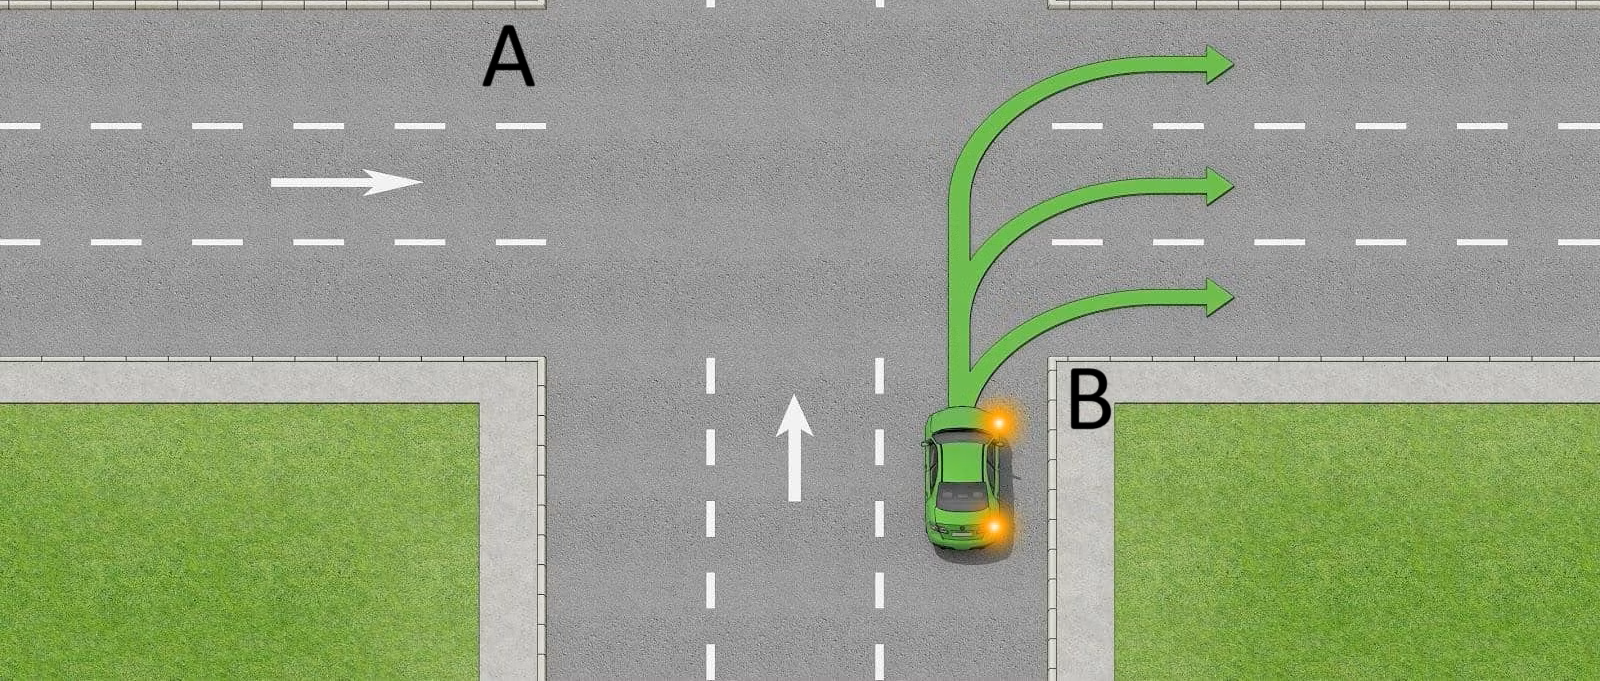
\includegraphics[width=0.75\linewidth]{images/Estrada_3.png}
    \caption[Traffic control of two roads by a traffic light.]{Traffic control of two roads by a traffic light~\cite{Abate2021}.}
    \label{fig:sinal}
\end{figure}

To translate this system into the IMITATOR syntax, it is necessary to represent events and transitions over time using concepts such as \textbf{clocks}, \textbf{variables}, \textbf{states}, and \textbf{transitions}. As explained in the previous chapter, to build our model, we need to construct three essential blocks.

In the first block, we declare the clocks and variables (discrete, rational, or parameters), as shown in Listing \ref{lst:traffic_var}.

\begin{figure}[H]
    \centering
    \begin{lstlisting}[language=UPPAAL, caption={Annotation Block rewritten with new values}, label={lst:traffic_var}]
    var
    x1, x2 : clock;
    
    T1_Green : parameter;
    T2_Green : parameter;
    T1_Yellow : parameter;
    T2_Yellow : parameter;
    T1_Red : parameter;
    T2_Red : parameter; 
    \end{lstlisting}
\end{figure}



The variables \texttt{x1} and \texttt{x2} are the internal counters of each traffic light, while the parameters, i.e., the variables, represent the thresholds for the duration each light can stay in each color. In this example, these times are not specifically defined, allowing the tool to optimize them as needed.


The next step is to construct the automata, defining their behavior using the previously declared clocks and variables. To improve readability, the automaton for Traffic Light 1 (Listing \ref{lst:sem_1}) is presented separately from the automaton for Traffic Light 2 (Listing \ref{lst:sem_2}).

%\begin{figure}[H]
%    \centering
    \begin{lstlisting}[language=UPPAAL, caption={Annotation Block rewritten with new values}, label={lst:sem_1}]
    (* Traffic Light 1 *)
    automaton Sem1
    synclabs: Go_Y;
    
    loc Green1:
      invariant x1 <= T1_Green
      when x1 = T1_Green sync Go_Y do {x1 := 0} goto Yellow1;
    
    loc Yellow1:
      invariant x1 <= T1_Yellow
      when x1 = T1_Yellow do {x1 := 0} goto Red1;
    
    loc Red1:
      invariant x1 <= T1_Red
      when x1 = T1_Red sync Go_Y do {x1 := 0} goto Green1;
    
    end
    \end{lstlisting}
%\end{figure}



%\begin{figure}[H]
%    \centering
    \begin{lstlisting}[language=UPPAAL, caption={Annotation Block rewritten with new values}, label={lst:sem_2}]
    (* Traffic Light 2 *)
    automaton Sem2
    synclabs: Go_Y;
    
    loc Green2:
      invariant x2 <= T2_Green
      when x2 = T2_Green sync Go_Y do {x2 := 0} goto Yellow2;
    
    loc Yellow2:
      invariant x2 <= T2_Yellow
      when x2 = T2_Yellow do {x2 := 0} goto Red2;
    
    loc Red2:
      invariant x2 <= T2_Red
      when x2 = T2_Red sync Go_Y do {x2 := 0} goto Green2;
    
    end
    \end{lstlisting}
%\end{figure}

\paragraph{}

Two automata have been declared, one for each traffic light. The behavior of both is very similar: in each state (green, yellow, red), there is an invariant condition that ensures the time each traffic light stays in each color will not be exceeded. Since the time values are parameters, they do not yet have a concrete value defined.

When the time limit for traffic light A's color is reached, the guard condition is triggered, initiating the color alternation between the two traffic lights. This resets both timers, synchronizing the transition of traffic light B, even if, in this case, the guard condition has not been directly validated.We can think of traffic light A as the master and traffic light B as the slave, ensuring that they can never be red or green simultaneously.

To better understand and summarize the model, we have constructed transition tables that represent the different system states, the invariants associated with each state, the conditions required for a transition to occur (guards), the synchronization events that trigger state changes, and the resulting next state for each transition. These tables provide a clear visualization of the automaton's logic, making it easier to analyze the system's behavior and ensuring that all timing constraints and synchronization events are properly followed.

\begin{table}[h!]
\centering
\begin{tabular}{|l|l|l|l|l|}
\hline
\textbf{State}  & \textbf{Invariant}      & \textbf{Guard}          & \textbf{Synchronized Event} & \textbf{Next State} \\ \hline
\texttt{Green1}  & $x_1 \leq T1\_Green$   & $x_1 = T1\_Green$       & \texttt{Go\_Y}        & \texttt{Yellow1}   \\ \hline
\texttt{Yellow1} & $x_1 \leq T1\_Yellow$  & $x_1 = T1\_Yellow$      & None                     & \texttt{Red1}      \\ \hline
\texttt{Red1}    & $x_1 \leq T1\_Red$     & $x_1 = T1\_Red$         & \texttt{Go\_Y}        & \texttt{Green1}    \\ \hline
\end{tabular}
\caption{Transition table for Traffic Light 1 (Sem1)}
\end{table}

\begin{table}[h!]
\centering
\begin{tabular}{|l|l|l|l|l|}
\hline
\textbf{State}  & \textbf{Invariant}      & \textbf{Guard}          & \textbf{Synchronized Event} & \textbf{Next State} \\ \hline
\texttt{Green2}  & $x_2 \leq T2\_Green$   & $x_2 = T2\_Green$       & \texttt{Go\_Y}        & \texttt{Yellow2}   \\ \hline
\texttt{Yellow2} & $x_2 \leq T2\_Yellow$  & $x_2 = T2\_Yellow$      & None                     & \texttt{Red2}      \\ \hline
\texttt{Red2}    & $x_2 \leq T2\_Red$     & $x_2 = T2\_Red$         & \texttt{Go\_Y}        & \texttt{Green2}    \\ \hline
\end{tabular}
\caption{Transition table for Traffic Light 2 (Sem2)}
\end{table}

\paragraph{}

Finally, we need to declare the initial positions of each automaton, initialize the variables, and set limits for them or for the timers (if applicable):

% \begin{lstlisting}[language=UPPAAL]
%     init := {
%         discrete = 
%             (*INITIAL LOCATION*)
%             loc[Sem1] := Green1,
%             loc[Sem2] := Red2,
    
%         ;
%         continuous =
%             (*INITIAL CLOCKS*)
%             & x1 = 0
%     	       & x2 = 0
            

%             (*PARAMETER CONSTRAINTS*)
%             & T1_Green > 0
%             & T2_Green > 0
%             & T1_Yellow > 0
%             & T2_Yellow > 0
%             & T1_Red > 0
%             & T2_Red > 0
%     	       & T1_Green = T2_Green + 60
%         ;

%     }
% \end{lstlisting}

\begin{lstlisting}[language=UPPAAL]
    init :=
            (*INITIAL LOCATION*)
          & loc[Sem1] := Green1
          & loc[Sem2] := Red2
            (*INITIAL CLOCKS*)
          & x1 = 0
          & x2 = 0
            (*PARAMETER CONSTRAINTS*)
          & T1_Green > 0
          & T2_Green > 0
          & T1_Yellow > 0
          & T2_Yellow > 0
          & T1_Red > 0
          & T2_Red > 0
          & T1_Green = T2_Green + 60;
\end{lstlisting}



\paragraph{}
As explained in the previous chapter, this part of the code is subdivided into discrete and continuous sections. It is important to highlight that, in the continuous part, an extra condition is added to the parameters: they must not only be greater than 0, but also the time that traffic light 1 stays green must be at least one minute longer than the time that traffic light 2 stays green.

As in the previous examples, we convert our model code into a visual representation as we can see in the Figure \ref{fig:TF_PTA}.

\paragraph{}

\begin{figure} [H]
    \centering
    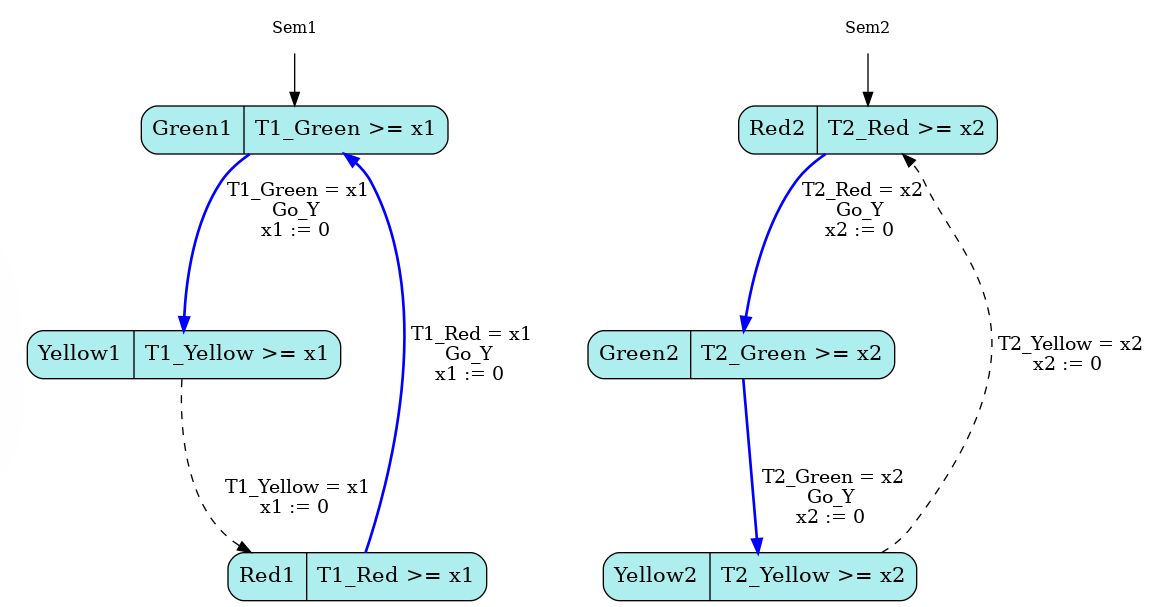
\includegraphics[width=1.05\linewidth]{images/Sem_pta.png}
    \caption[Traffic Light Automata]{Traffic Light Automata}
    \label{fig:TF_PTA}
\end{figure}

%\subsubsection{System Analysis}

%Com o modelo construído procedemos á verificação das propriedades tal como no exemplo anterior e já tendo as propriedades guardadas num ficheiro .imiprop separado do modelo. Começamos pela verificação da não ocorrência de deadlock sendo que usamos a seguinte syntax : property := synth DeadlockFree;




\paragraph{}
\paragraph{}
\end{comment}

\subsection{Coffee Machine}

First, we have a Coffee Machine system. To simplify, it is assumed that this machine does not require coins or any other mechanism to start the process; it only has 1 button to initiate the process. This button is also used to add sugar to the coffee.

\begin{figure} [H]
    \centering
    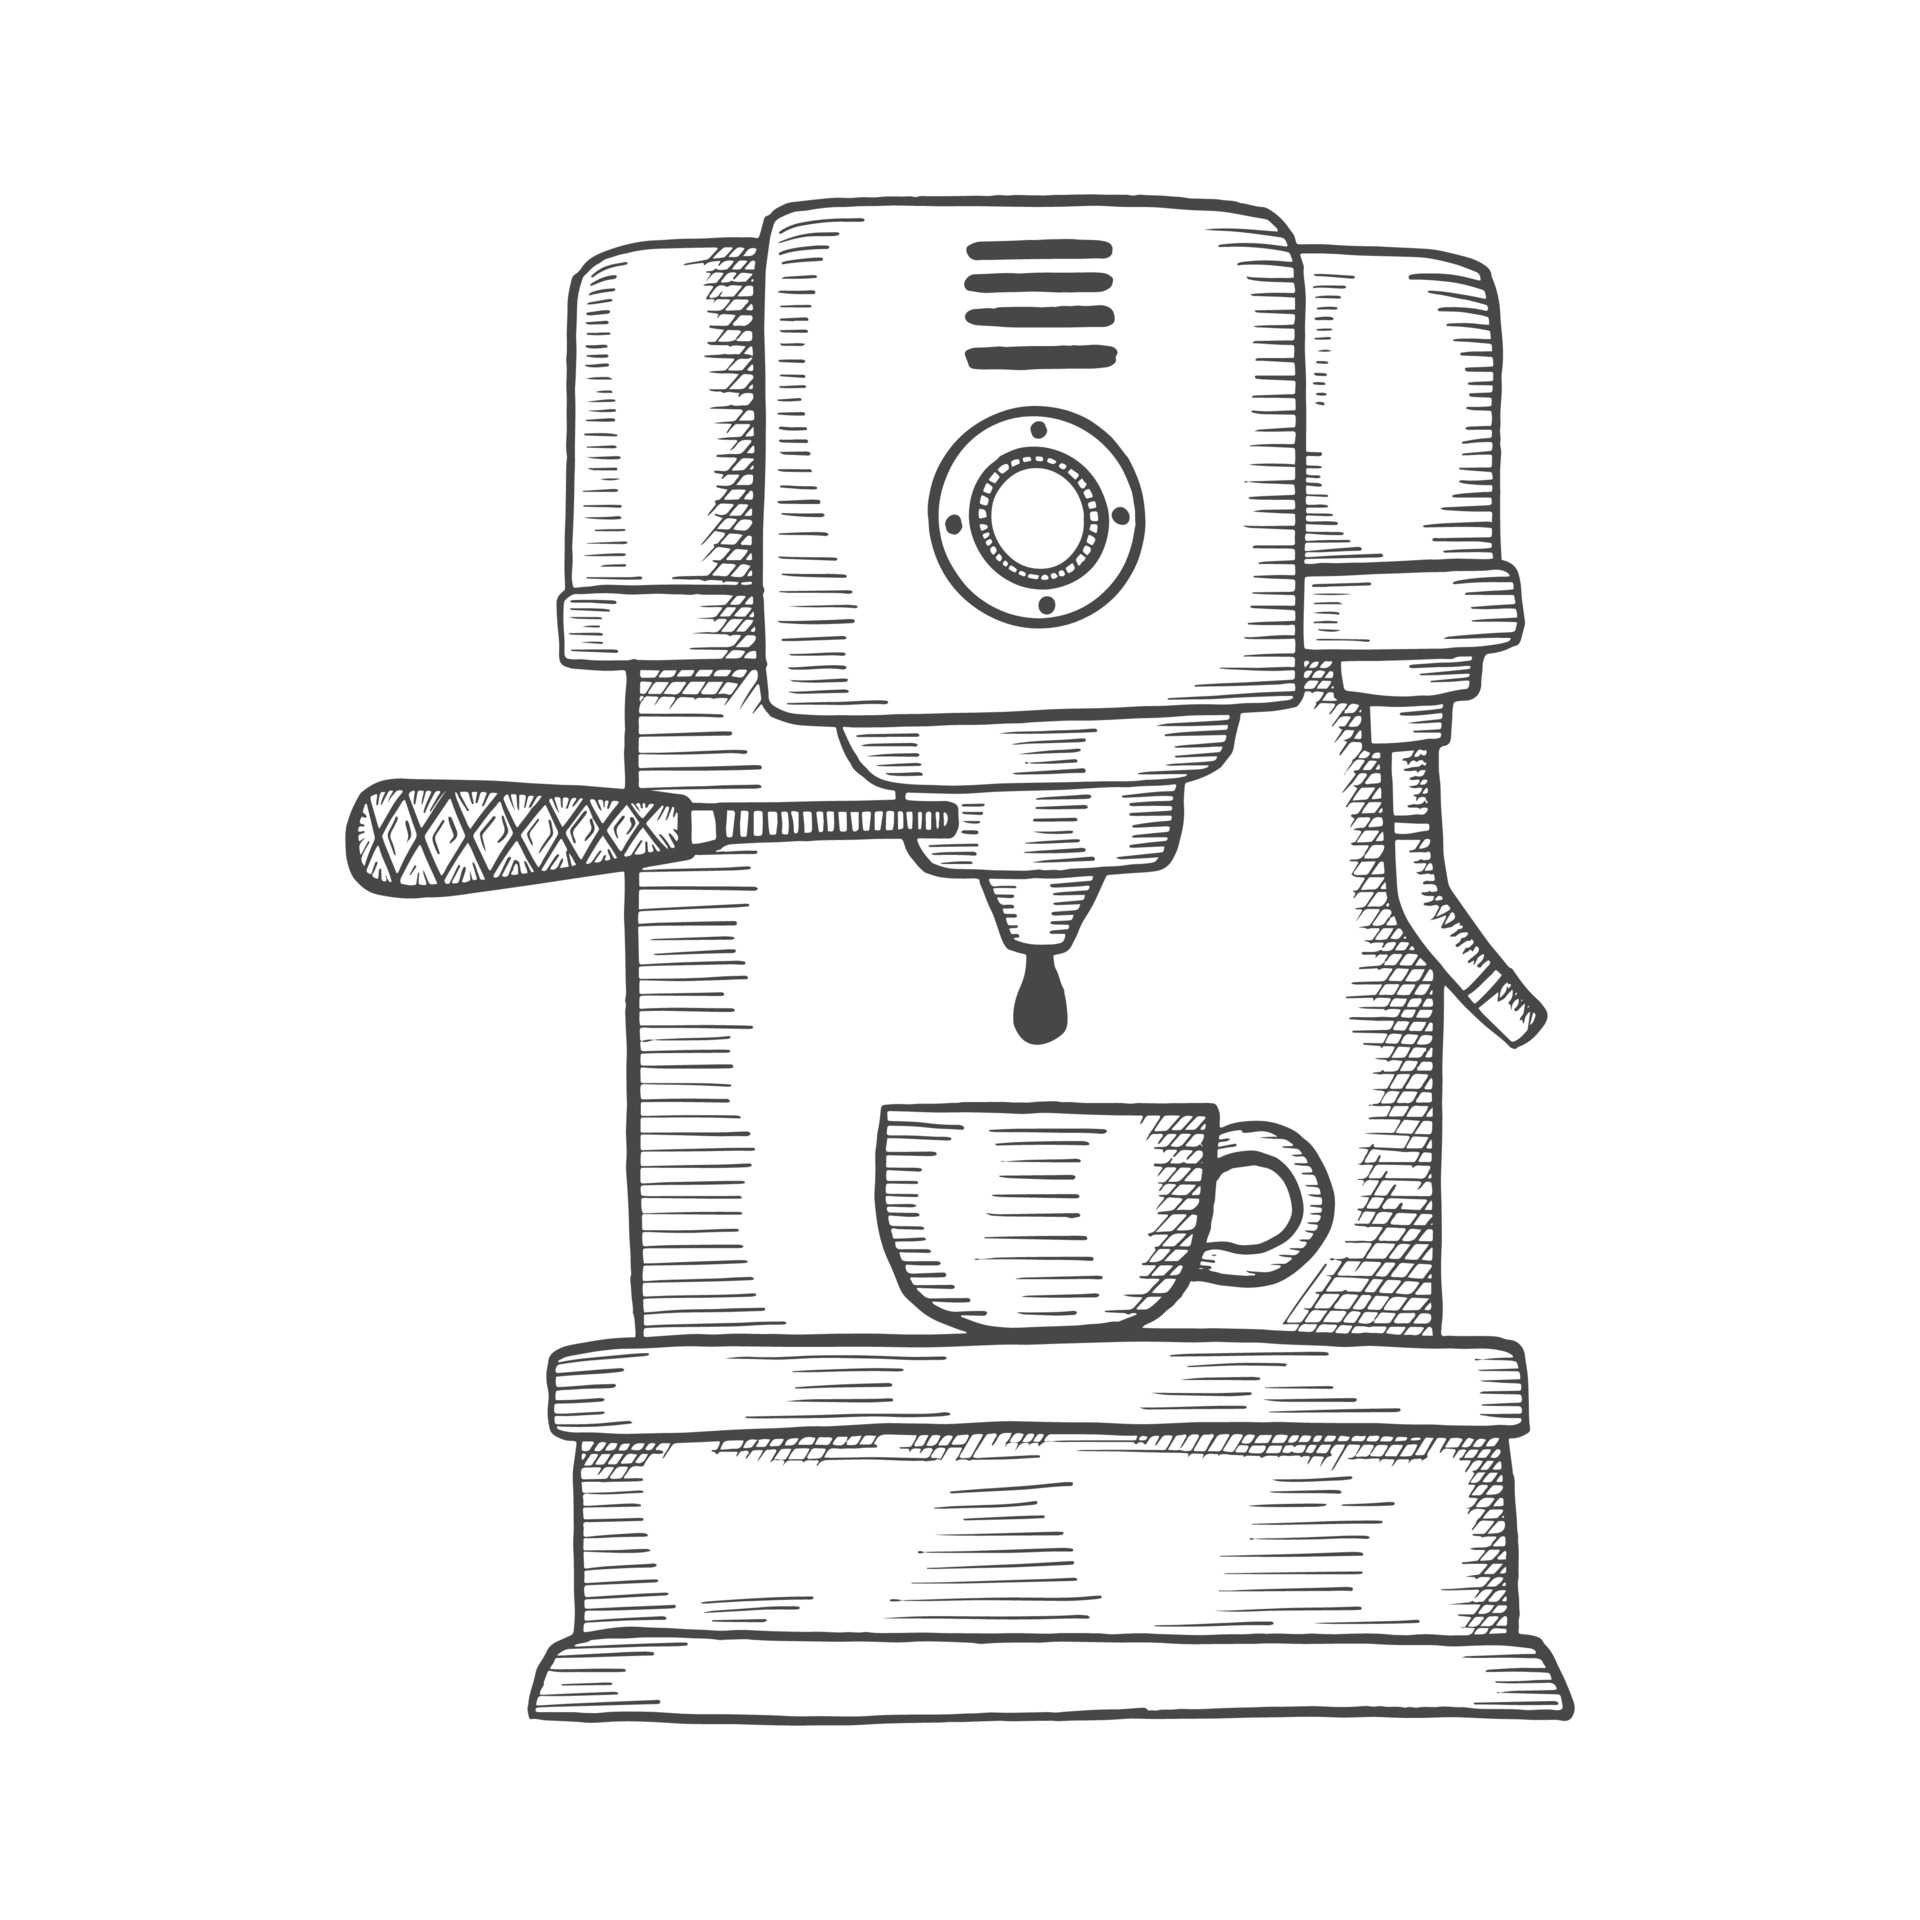
\includegraphics[width=0.4\linewidth]{chapters/vecteezy_coffee-espresso-machine-lover-single-isolated-hand-drawn_8148187.jpg}
    \caption[Simple Coffee Machine with only one button to control all operations.]{Simple Coffee Machine with only one button to control all operations.~\cite{Abate2021}}
    \label{fig:modelcheckingC}
\end{figure}

\paragraph{}

To translate this system into the IMITATOR syntax, it is necessary to represent events and transitions over time using concepts such as \textbf{clocks}, \textbf{variables}, \textbf{states}, and \textbf{transitions}. As explained in the previous chapter, to build our model, we need to construct three essential blocks.

In the first block, we declare the clocks and variables (discrete, rational, or parameters):

\begin{lstlisting}[language=UPPAAL]
    var  x, y       : clock;
         p1, p2, p3 : parameter;
\end{lstlisting}

The variable \textbf{p1} represents the time elapsed between two consecutive sugar requests after the process has started. In other words, it is the interval between each request made by the user to add sugar to the coffee. The variable \textbf{p2} defines the time window during which the user can press the button again to request more sugar. If the system allows this additional request, it will wait for user interaction within this interval before proceeding with the process. Finally, the variable \textbf{p3} corresponds to the time required to produce and serve the coffee. This period includes all steps from the beginning of the preparation until the moment the beverage is served to the user.

\paragraph{}

The next step is the construction of the automaton. In this case, a single automaton will be developed to represent the operation of the coffee machine.

\begin{lstlisting}[language=UPPAAL]
    (*Coffe Machine*)
    synclabs: press, cup, coffee, sleep;

    loc idle: invariant True
    	when True sync press do {x := 0, y := 0} goto add_sugar;
    
    loc add_sugar: invariant y <= p2
    	when x >= p1 sync press do {x := 0} goto add_sugar;
    	when y = p2 sync cup do {} goto preparing_coffee;
    
    loc preparing_coffee: invariant y <= p3
    	when y = p3 sync coffee do {x := 0} goto cdone;
    
    accepting loc cdone: invariant x <= 10
    	when True sync press do {x := 0, y := 0} goto add_sugar;
    	when x = 10 sync sleep goto idle;
    
    end
\end{lstlisting}


The coffee machine's automaton consists of four states. The first state is \textbf{Standby(\textit{idle})}, where the system waits indefinitely for the user to take action to start making coffee. The next state is \textbf{\textit{add\_sugar}}, where the user can choose to add sugar. There is a time limit (p₂) for adding sugar, and a restriction (p₁) on how often sugar can be added in quick succession. These restrictions are enforced using invariants, in the state add\_sugar, with the invariant y ≤ p₂ and in the preparing\_coffee state with the invariant y ≤ p₁.The synchronization here is based on the \textit{press} event, which triggers the action of adding sugar and starts the process. Next is the coffee preparation state\textbf{(\textit{preparing\_coffee})}, which takes p₃ time units to complete. The synchronization with the coffee event triggers the completion of the coffee preparation. Finally, in the last state(\textbf{\textit{cdone}}), if the user presses the button again within 10 time units, the system goes back to add\_sugar and repeats the process. This synchronization is triggered by the \textit{press} event. If the user does not press the button within the allowed time, the system synchronizes with the \textit{sleep} event, returning to the Standby state.

It is important to note that the last state, called the \textbf{\textit{accepting loc}}, is different from the others because it represents a 'final' or 'accepting' state. In simple terms, once the system reaches this state, the coffee is prepared and ready to be served. This distinction is useful during the verification process, as it allows us to check whether the automaton can reach a successful end state instead of getting stuck in infinite loops within intermediate states \cite{IMITATOR}.

The model is summarized in Transition Table \ref{tab:automato_cafe}.

\paragraph{}



\begin{table}[h!]
\centering
\resizebox{\textwidth}{!}{
\begin{tabular}{|l|l|l|l|l|l|}
\hline
\textbf{State}             & \textbf{Invariant}     & \textbf{Guard}         & \textbf{Synchronized Event} & \textbf{Action}              & \textbf{Next State}       \\ \hline
\texttt{idle}              & Always (\texttt{True})  & Always (\texttt{True}) & \texttt{press}        & \texttt{x := 0, y := 0}  & \texttt{add\_sugar}       \\ \hline
\texttt{add\_sugar}        & $y \leq p_2$           & $x \geq p_1$           & \texttt{press}        & \texttt{x := 0}          & \texttt{add\_sugar}       \\ \hline
\texttt{add\_sugar}        & $y \leq p_2$           & $y = p_2$              & \texttt{cup}          & None           & \texttt{preparing\_coffee} \\ \hline
\texttt{preparing\_coffee} & $y \leq p_3$           & $y = p_3$              & \texttt{coffee}       & \texttt{x := 0}          & \texttt{cdone}            \\ \hline
\texttt{cdone} & $x \leq 10$            & Always (\texttt{True}) & \texttt{press}        & \texttt{x := 0, y := 0}  & \texttt{add\_sugar}       \\ \hline
\texttt{cdone}            & $x \leq 10$            & $x = 10$               & \texttt{sleep}        & None           & \texttt{idle}             \\ \hline
\end{tabular}
}
\caption{Transition table of the coffee machine automaton.}
\label{tab:automato_cafe}
\end{table}



To complete the model, it is necessary to declare the initial states as well as the possible constraints on the clocks and declared variables:

\begin{lstlisting}[language=UPPAAL]
    init :=
    	(* Initial location *)
    	& loc[machine] = idle
    	(* Initial clock constraints *)
    	& x = 0
    	& y = 0
    	(* Parameter constraints *)
    	& p1 >= 0
    	& p2 >= 0
    	& p3 >= 0
    ;
\end{lstlisting}



The initial location, as explained earlier, is set to the \textit{idle} state, meaning Standby mode. Additionally, the clocks are initialized to 0, and the parameters must be positive.

\paragraph{}

To verify whether our system complies with the syntax, we can, as explained in the previous chapter, run the model in the command line with the option to translate the system into a PNG image using the following command: \texttt{./imitator mod.imi -imi2PNG}

If this command fails, it means that our model has syntax errors that need to be fixed.

Considering that we saved our model in the \textbf{mod.imi} file, we obtain the following image as output in Figure \ref{fig:cof_output}, which visually represents our code.




\begin{figure} [H]
    \centering
    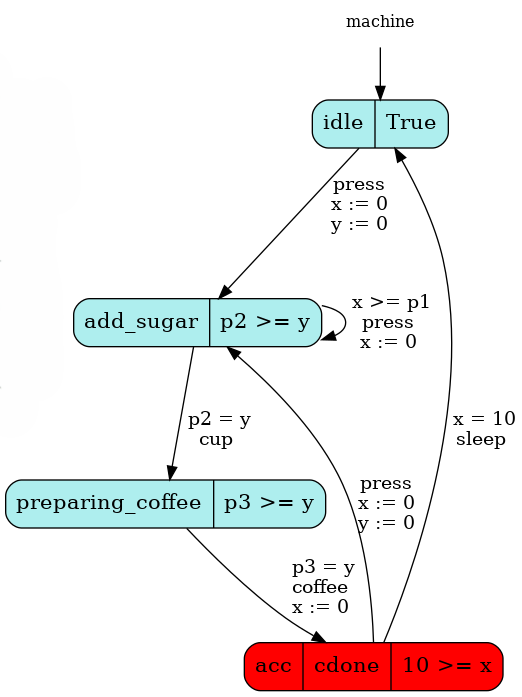
\includegraphics[width=0.55\linewidth]{images/sys.png}
    \caption[Coffee Machine Automata]{Coffee Machine Automata}
    \label{fig:cof_output}
\end{figure}




\subsubsection{System Analysis}

Once the model is built, we can proceed to property verification. We start with parameter synthesis to ensure that deadlocks are avoided. To achieve this, we need to create a separate \texttt{.imiprop} file, distinct from the .imi file containing our model, as explained in the previous chapter.


Inside the file, we define the property to be verified. In this case, related to deadlock. The syntax is as follows : \texttt{property := \#synth DeadlockFree;}

The result is stored in a \texttt{.res} file with the same name as the file where the model is saved. This file contains general information about the model as well as the verification of the property. However, the most important part we extract is the following:

\begin{verbatim}
     p1 >= 0
    & p2 >= 0
    & p3 >= p2
    OR
      p2 > p3
    & p3 >= 0
    & p1 = 0
\end{verbatim}

Any values chosen for the parameters, as long as they satisfy the given constraint, ensure that the system does not reach a deadlock. We can also determine the maximum or minimum parameter value that ensures a given property is satisfied. For example, we may want to find the shortest possible time between two consecutive sugar requests(\( p1 \)) while still allowing the coffee to be served to the user (i.e., reaching the location \texttt{cdone}).

To achieve this, we can use the following property: 
\texttt{property := \#synth EFpmin(loc[machine] = cdone, p1);} With this property, we obtain the following result:

\begin{verbatim}
     p3 >= p2
     & p2 >= 0
     & p1 = 0
\end{verbatim}

The parameter \( p1 \) can be 0, meaning that the request for sugar can be made instantly. However, this is only possible as long as the time required to prepare a coffee (\( p1 \)) is greater than the time interval in which sugar can be requested (\( p2 \)). Additionally, \( p2 \) must be strictly positive to ensure a valid sequence of events.

A synthesis of both verified properties can be found in the table \ref{tab:property_results}

\begin{table}[h!]
\centering
\resizebox{\textwidth}{!}{
\begin{tabular}{|p{5cm}|l|p{5cm}|}
\hline
\textbf{Property} & \textbf{Meaning} & \textbf{Result} \\ \hline
\texttt{property := synth DeadlockFree;} & Ensures the system does not reach a deadlock state. & 
\begin{minipage}[t]{8cm}
$p_1 \geq 0 \land p_2 \geq 0 \land p_3 \geq p_2$\\
\textbf{or}\\
$p_2 > p_3 \land p_3 \geq 0 \land p_1 = 0$
\end{minipage} \\ \hline

\texttt{property := \#synth EFpmin(loc[machine] = cdone, p1);} & Finds the minimum value of $p_1$ to reach location \texttt{cdone}. &
\begin{minipage}[t]{8cm}
$p_3 \geq p_2$\\
$p_2 \geq 0$\\
$p_1 = 0$
\end{minipage} \\ \hline
\end{tabular}
}
\caption{Synthesis of properties and corresponding results.}
\label{tab:property_results}
\end{table}


\subsection{Worker and Hammer System}

Now we have the "Worker and Hammer" system, as discussed in the State of the Art chapter and implemented in UPPAAL. This system represents the interaction between a worker and a hammer to perform a repetitive task, such as hammering nails.

As in the other examples, we start by defining the variables and clocks of the automata.

\begin{lstlisting}[language=UPPAAL]
    var
    session, t
    :clock;
    
    sessionTime,
    reactTime,
    totalNails
    : parameter;
    nails
    : int;	
\end{lstlisting}


The \textbf{t} and \textbf{session} timers are used to measure elapsed time for different purposes. The t timer tracks short-duration actions, such as hammering a nail or placing a new one, while the session timer records the total time a worker has spent working in a session, determining when the worker need to take a break. The variables \textbf{sessionTime}, \textbf{reactTime}, and \textbf{totalNails} are defined as parameters, unlike in the UPPAAL example, where they had fixed values. \textbf{sessionTime} represents the maximum time a worker can work before stopping, \textbf{reactTime} is the maximum time allowed for the worker to hit or place a new nail, and \textbf{totalNails} indicates the total number of new nails available. Finally, the variable \textbf{Nails} is defined as a discrete type, specifically an integer, and serves as an accumulator for the number of completed nails. Its value is initialized to 0 in the final section of the code. With all variables declared, the next step is the definition of the automata.
%\paragraph{}

\begin{lstlisting}[language=UPPAAL]
    (*Worker Automata*)
    automaton Worker
    
    synclabs: rest, hit, newNail, Work;
    
    loc Rest: invariant session <= sessionTime - reactTime
      	when True sync Work do {t := 0} goto Work;
    
    loc Work: invariant session <= sessionTime && t <= reactTime
      	when t >= reactTime sync newNail do {t := 0} goto Work;
      	when t >= reactTime - 5 sync hit do {t := 0} goto Work;
      	when session >= sessionTime sync rest do {session := 0} goto Rest;
    
    end
    
    (*Hammer Automata*)
    automaton Hammer
    
    synclabs: hit, newNail;
    
    loc NailUp: invariant True
      	when True sync hit goto NailHalf;
    
    loc NailHalf: invariant True
      	when True sync hit do {nails := nails +1} goto NailDone;
    
    loc NailDone: invariant True
      	when nails <= totalNails sync newNail goto NailUp;
    
    end


\end{lstlisting}


The system consists of two automata: \textbf{Worker} and \textbf{Hammer}. The \textbf{Worker} represents a worker who alternates between the states Rest and Work. In the Rest state, the worker waits for the start of work through the Work synchronization, resetting the clock t in the process. After this synchronization, in the Work state, the worker can perform two actions: hitting the nail (hit), if t ≥ reactTime - 5, or placing a new nail (newNail!), if t ≥ reactTime, always resetting t after each action. The worker can remain in the Work state as long as session < sessionTime. Once this limit is exceeded, the worker returns to the Rest state through the transition rest!, which also resets the session clock.

The \textbf{Hammer} automaton represents the interaction of the hammer with the nails, alternating between the states NailUp (new nail), NailHalf (partially hammered nail), and NailDone (completely hammered nail). Initially, it is in the NailUp state, where upon receiving the synchronization Hit, it transitions to NailHalf. Upon receiving a second synchronization Hit, it transitions to NailDone, incrementing the variable nails if countNails is activated. When the nail is completely hammered, the system can insert a new nail through the synchronization newNail?, returning to the NailUp state, provided that infiniteNails is true or nails < totalNails. 

The synchronization between the two automata occurs through the channels Hit and newNail presented in the Worker and Hammer automata, ensuring that the sequence of events is consistent and respects the temporal constraints imposed by the clocks t and session.

We can better visualize the behavior of the Worker automaton in Table \ref{tab:wh_t1} and of the Hammer automaton in Table \ref{tab:wh_t2}.
\paragraph{}

\begin{table}[h!]
\centering
\resizebox{\textwidth}{!}{
\begin{tabular}{|l|l|l|l|l|l|}
\hline
\textbf{State}             & \textbf{Invariant}            & \textbf{Guard}                & \textbf{Synchronized Event} & \textbf{Action}               & \textbf{Next State}         \\ \hline
\texttt{Rest}              & Always (\texttt{True})         & session $\leq$ sessionTime - reactTime & \texttt{work!}              & \texttt{session := 0}         & \texttt{Work}               \\ \hline
\texttt{Work}              & session $\leq$ sessionTime     & t $\leq$ reactTime            & \texttt{newNail!}            & \texttt{t := 0}               & \texttt{Work}               \\ \hline
\texttt{Work}              & session $\leq$ sessionTime     & t $\geq$ reactTime - 5        & \texttt{hit!}                & \texttt{t := 0}               & \texttt{Work}               \\ \hline
\texttt{Work}              & session $\geq$ sessionTime     & None                              & \texttt{rest!}               & \texttt{session := 0}         & \texttt{Rest}               \\ \hline
\end{tabular}
}
\caption[Worker Transistion Table]{Worker Transistion Table}
\label{tab:wh_t1}
\end{table}
 
\begin{table}[h!]
\centering
\resizebox{\textwidth}{!}{
\begin{tabular}{|l|l|l|l|l|l|}
\hline
\textbf{State}             & \textbf{Invariant}            & \textbf{Guard}                & \textbf{Synchronized Event} & \textbf{Action}               & \textbf{Next State}         \\ \hline
\texttt{NailUp}            & Always (\texttt{True})         & nails $\leq$ totalNails or infiniteNails & \texttt{newNail?}            & None                          & \texttt{NailHalf}           \\ \hline
\texttt{NailHalf}          & Always (\texttt{True})         & None                              & \texttt{hit?}                & \texttt{nails++}              & \texttt{NailDone}           \\ \hline
\texttt{NailDone}          & Always (\texttt{True})         & None                              & \texttt{newNail?}            & None                          & \texttt{NailUp}             \\ \hline
\end{tabular}
}
\caption[Hammer Transistion Table]{Hammer Transistion Table}
\label{tab:wh_t2}
\end{table}

Finally, we just need to declare the initial states of the automata, which are Rest and NailUp for the Worker and Hammer, respectively. Additionally, we initialize the clocks and the nails variable to 0, and set the condition that the parameters must be greater than 0.

\begin{lstlisting}[language=UPPAAL]
    init := 
  
    & loc[Worker] = Rest
    & loc[Hammer] = NailUp
    
    & session = 0
    & t = 0
    
    & nails = 0
    & sessionTime >= 0
    & reactTime >= 0
    ;
    end
\end{lstlisting}


As in the previous examples, we convert our model code into a visual representation.

\begin{figure} [H]
    \centering
    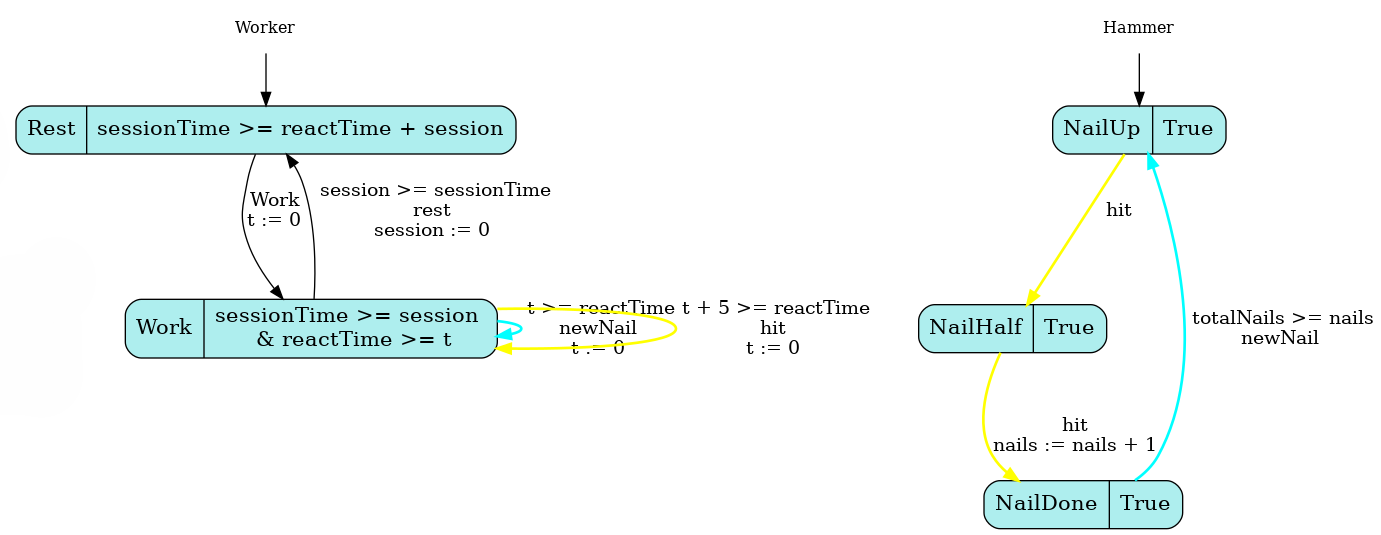
\includegraphics[width=1\linewidth]{images/WH-PTA.png}
    \caption[Worker and Hammer Automata]{Worker and Hammer Automata}
    \label{fig:cof_output}
\end{figure}




\subsubsection{System Analysis}

As before, we start by determining the parameter values needed to avoid a deadlock. In other words, we analyze how the worker's working time, the time required to hammer or place a new nail, and the number of nails must be set to prevent this situation. The property, as previously mentioned, is stored in a separate \texttt{.imiprop} file and has the following syntax: \texttt{property := synth DeadlockFree;} Analyzing the \texttt{.res} file, the parametric interval that guarantees the absence of deadlock is as follows:

\begin{verbatim}
     0 > reactTime
    & sessionTime >= 0
    OR
      reactTime >= sessionTime
    & sessionTime >= 0
\end{verbatim}

We can also determine the parametric interval that guarantees the completion of the worker's action—that is, ensuring that the location NailDone in the Hammer automaton is reachable. For this, we use a simple Reachability property with the following syntax: \texttt{property := \#synth EF(loc[Hammer] = NailDone);}

The parametric interval is of the form:

\begin{verbatim}
     reactTime >= 0
    & sessionTime >= reactTime
\end{verbatim}

To ensure that the completion of the action is guaranteed, reactTime must be a positive value, and additionally, it must be ensured that sessionTime is always greater than or equal to reactTime. Table \ref{tab:property_results} summarizes the verified properties and their corresponding synthesis results. The first property ensures that the system avoids deadlock by constraining the parameters \texttt{reactTime} and \texttt{sessionTime}. The second property determines the conditions under which the system can reach the target location \texttt{cdone}, ensuring progress towards the completion of the task. Together, these results confirm that the model behaves correctly within the specified parameter ranges.


\begin{table}[h!]
\centering
\resizebox{\textwidth}{!}{
\begin{tabular}{|p{5cm}|l|p{5cm}|}
\hline
\textbf{Property} & \textbf{Meaning} & \textbf{Result} \\ \hline
\texttt{property := synth DeadlockFree;} & Ensures the system does not reach a deadlock state. & 
\begin{minipage}[t]{8cm}
$reactTime > 0  \\
\land sessionTime \geq 0$\\
\textbf{or}\\
$sessionTime \geq reactTime \\
\land sessionTime \geq 0$
\end{minipage} \\ \hline

\texttt{property := \#synth EF(loc[Hammer] = NailDone);} & Finds the minimum value of $p_1$ to reach location \texttt{cdone}. &
\begin{minipage}[t]{8cm}
$reactTime \geq 0$\\
$\land sessionTime \geq reactTime$\\
\end{minipage} \\ \hline
\end{tabular}
}
\caption{Synthesis of properties and corresponding results.}
\label{tab:property_results}
\end{table}


\subsection{ATM Machine}

The final example is of a simple ATM with only two functions: balance inquiry and cash withdrawal, considering time constraints for each phase of the operation. The example was also taken from the official Imitator website \cite{IMITATOR}. We begin by declaring the system's variables and clocks:

%\begin{figure} [H]
%    \centering
%    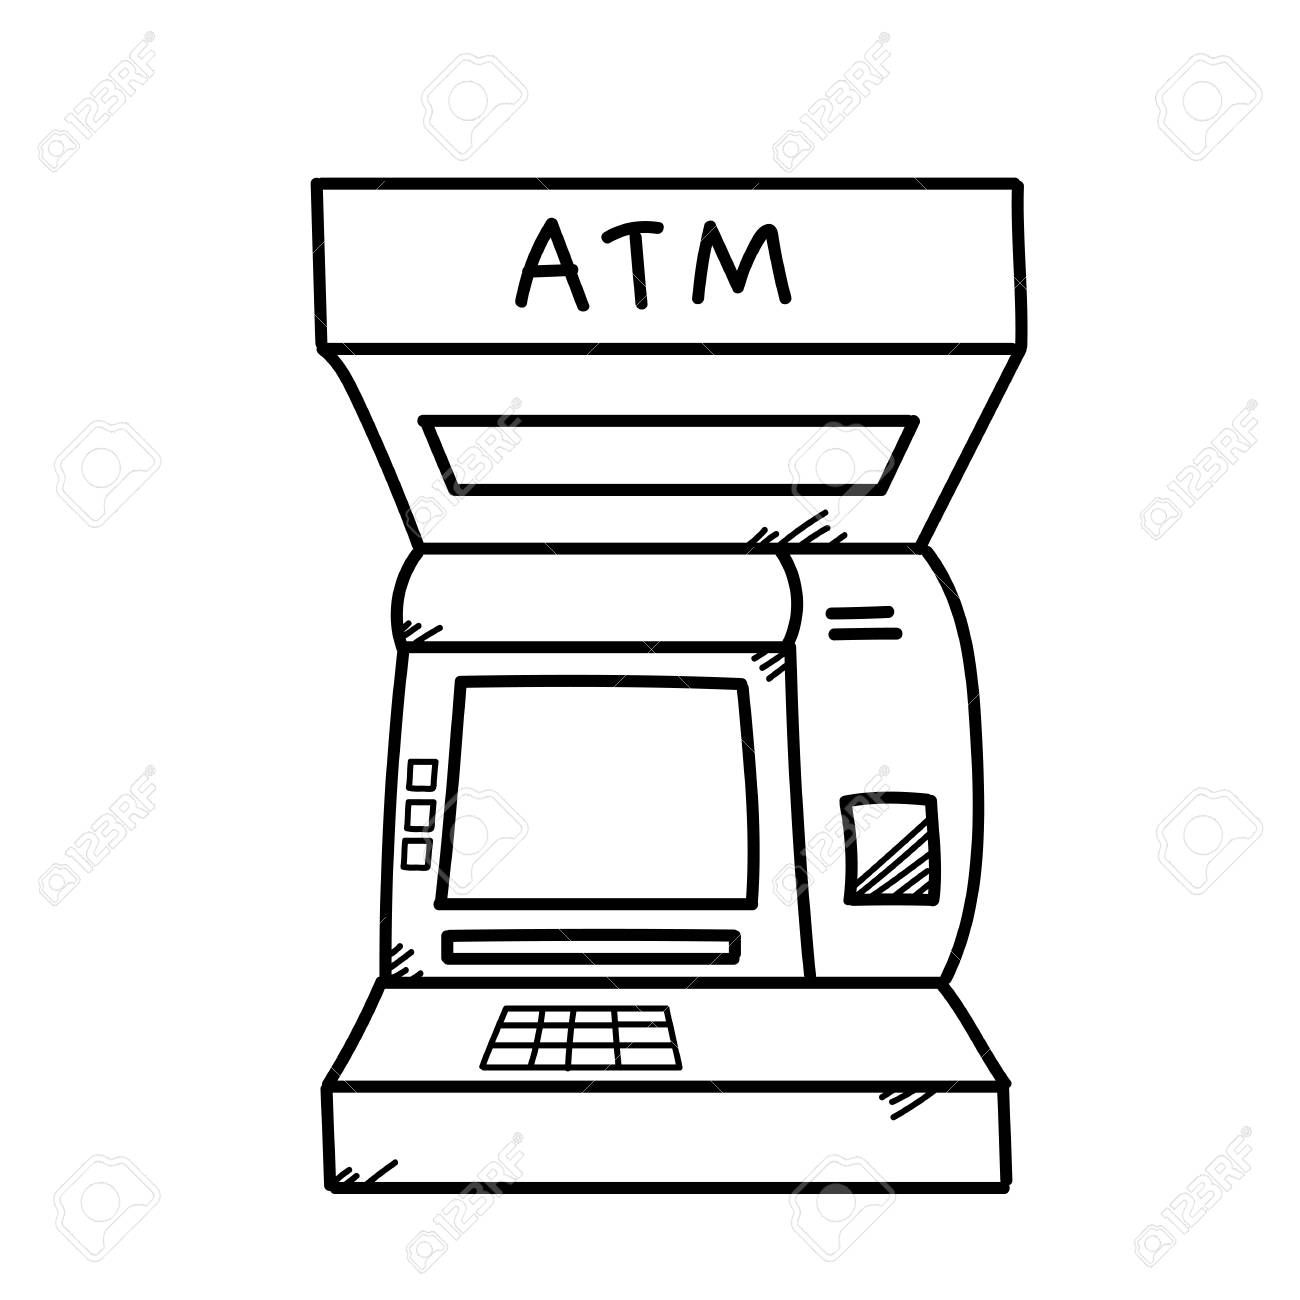
\includegraphics[width=0.4\linewidth]{images/ATM.jpg}
%    \caption[ATM Machines.]{ATM Machine.\cite{amisb2018atm}}
%    \label{fig:ATM_IMI}
%\end{figure}

%\paragraph{}
\begin{lstlisting}[language=UPPAAL]
    var
    x,y,z : clock;

    p1 : parameter;
    p2 : parameter;
    p3 : parameter;
\end{lstlisting}


Clock x controls the duration of each operation and is used to limit the time allowed for the selected operation. For example, if x = 15 and the chosen operation is withdraw, the user has 15 time units to complete it. Clock y is responsible for tracking the login time, i.e., the time the user takes to provide access credentials.
Finally, clock z monitors the total session time (login + operations). Regarding the variables, they are all defined as parameters: p1 is the maximum allowed session time, p2 defines the maximum time for login, and p3 sets the maximum time allowed per operation, whether it is a balance inquiry or a withdrawal.

\begin{lstlisting}[language=UPPAAL]
    automaton pta
    
    synclabs: ;

    loc Idle: invariant True
    	when True do {x := 0 , y := 0 , z := 0} goto Start;
    
    loc Start: invariant z <= p1
    	when z = p1 goto Idle;
    	when z <= p1 do { y := 0 } goto Login;
    
    loc Login: invariant y <= p2 && z <= p1
    	when z = p1 goto Idle;
    	when True do {x := 0} goto Withdrawals;
    	when y = p2 goto Start;
    	when True do {x := 0} goto Check;
    
    loc Withdrawals: invariant x <= p3
    	when True goto Login;
    
    loc Check: invariant x <= p3
    	when True goto Login;
    
    end
\end{lstlisting}


The automaton is composed of five locations: Idle, Start, Login, Withdrawals, and Check. The initial state is Idle, which represents the ATM being in a standby state, waiting for the start of an operation. When this occurs, all clocks are reset to 0 and the automaton transitions to the Start location. This location marks the beginning of the user interaction. The invariant z <= p1 limits the session duration, with p1 representing the maximum session time; if this limit is exceeded, the system returns to the Idle state (standby). Otherwise, it proceeds to the Login state, where clock y is reset. This clock tracks the time the user takes to log in. In this location, the machine waits for the user to enter their credentials, with the constraint that the login duration must not exceed either of the specified time bounds, as indicated by the invariant \texttt{y <= p2 \&\& z <= p1}. If both conditions are satisfied, the system moves to the Withdrawals location if that was the selected function, or to Check otherwise. In both cases, clock x is reset. If the selected operation is Withdrawal, the system transitions to that location, giving the user a limited time to complete the withdrawal, which cannot exceed p3, as shown by the invariant \texttt{x <= p3}. If the option is Check, it moves to the corresponding location, where the same time restriction applies, also enforced by the invariant \texttt{x <= p3}. In both cases, after completing the action, the system returns to the Login location, allowing the user to repeat or change the selected operation. As with the previous examples, we can construct a transition table for the system, as shown in Figure \ref{tab:atm_tt}.

\begin{table}[h!]
\centering
\resizebox{\textwidth}{!}{
\begin{tabular}{|l|l|l|l|l|l|}
\hline
\textbf{State}         & \textbf{Invariant}                        & \textbf{Guard}          & \textbf{Synchronized Event} & \textbf{Action}                & \textbf{Next State}   \\ \hline
\texttt{Idle}          & Always (\texttt{True})                   & Always (\texttt{True})  & \texttt{start}              & \texttt{x := 0, y := 0, z := 0} & \texttt{Start}        \\ \hline
\texttt{Start}         & $z \leq p_1$                              & $z = p_1$               & \texttt{timeout}            & None                           & \texttt{Idle}         \\ \hline
\texttt{Start}         & $z \leq p_1$                              & $z \leq p_1$            & \texttt{proceed}            & \texttt{y := 0}                & \texttt{Login}        \\ \hline
\texttt{Login}         & $y \leq p_2 \wedge z \leq p_1$            & $z = p_1$               & \texttt{timeout}            & None                           & \texttt{Idle}         \\ \hline
\texttt{Login}         & $y \leq p_2 \wedge z \leq p_1$            & $y = p_2$               & \texttt{restart}            & None                           & \texttt{Start}        \\ \hline
\texttt{Login}         & $y \leq p_2 \wedge z \leq p_1$            & Always (\texttt{True})  & \texttt{withdraw}           & \texttt{x := 0}                & \texttt{Withdrawals}  \\ \hline
\texttt{Login}         & $y \leq p_2 \wedge z \leq p_1$            & Always (\texttt{True})  & \texttt{check}              & \texttt{x := 0}                & \texttt{Check}        \\ \hline
\texttt{Withdrawals}   & $x \leq p_3$                              & Always (\texttt{True})  & \texttt{done}               & None                           & \texttt{Login}        \\ \hline
\texttt{Check}         & $x \leq p_3$                              & Always (\texttt{True})  & \texttt{done}               & None                           & \texttt{Login}        \\ \hline
\end{tabular}
}
\caption{Transition table of the ATM automaton.}
\label{tab:atm_tt}
\end{table}

Finally, we define the parameter constraints and the initial location of the automaton.

\begin{lstlisting}[language=UPPAAL]
    init := 

    & loc[pta] = Idle,
    
    & x = 0
    & y = 0
    & z = 0

    & p1 >= 0
    & p2 >= 0
    & p3 >= 0
    ;

    end
\end{lstlisting}


As mentioned, the system starts in the Idle location, which represents the standby state. Additionally, the only constraint imposed on the parameters is that they must be greater than 0. As with the previous examples, we can convert the model into a figure, as shown in Figure \ref{fig:ATM_output}.


\begin{figure} [H]
    \centering
    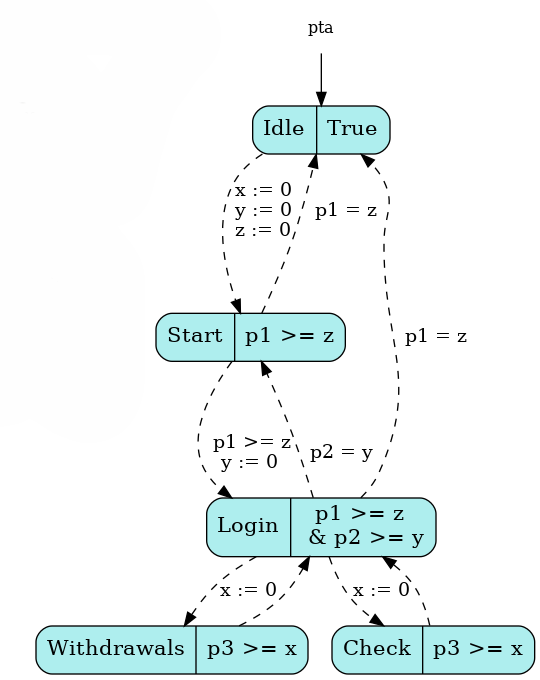
\includegraphics[width=0.6\linewidth]{images/fixed.png}
    \caption[ATM Automata]{ATM Automata}
    \label{fig:ATM_output}
\end{figure}

\subsubsection{System Analysis}

As in the previous examples, the first property to be verified is deadlock-freedom, ensuring that the system does not reach any state from which execution cannot proceed. The syntax for this property, as previously mentioned, is: \texttt{property := synth DeadlockFree}. The parametric interval that guarantees the verification of the property is as follows:

\begin{verbatim}
    p3 >= 0
    & p2 >= 0
    & p1 >= 0
\end{verbatim}

It tell that whatever values the parameters may take, it must be ensured that they are always positive in order to guarantee that "regardless of the situation, the system always has an action to take."

The next property to be verified is a liveness property that searches for at least one cycle in the automaton that goes through the Withdrawals state and can be executed infinitely (i.e., without deadlock). In practical terms, this ensures that it is always possible to perform withdrawals. For this purpose, we use the CycleThrough algorithm, which was briefly mentioned in the previous chapter. The corresponding syntax is: \texttt{property := synth CycleThrough(loc[pta] = Withdrawals);}. The returned parametric interval guarantees that the cycle exists for any non-negative values of parameters p1, p2, and p3.

\begin{verbatim}
    p3 >= 0
    & p2 >= 0
    & p1 >= 0
\end{verbatim}

Additionally, Imitator provides extra information such as the depth at which the cycle was found (i.e., the number of transitions required to complete it), as well as the number of states generated and effectively explored during the analysis.

A summary of the analyzed properties and their corresponding results can be found in Table \ref{tab:property_results_atm}.

\begin{table}[h!]
\centering
\resizebox{\textwidth}{!}{
\begin{tabular}{|p{5cm}|l|p{2cm}|}
\hline
\textbf{Property} & \textbf{Meaning} & \textbf{Result} \\ \hline
\texttt{property := \#synth DeadlockFree;} &
    Ensures the system does not reach a deadlock state. & 
    \begin{minipage}[t]{8cm}
    $p_1 > 0  \\
    \land p_2 \geq 0\\
    \land p_3 \geq 0$\\
    \end{minipage}
\\\hline

\texttt{property := \#synth CycleThrough(loc[pta] = Withdrawals);} & Find a cycle in which the Withdrawals location is visited. \texttt{cdone}. &
\begin{minipage}[t]{4cm}
$p_1 > 0  \\
\land p_2 \geq 0\\
\land p_3 \geq 0$\\
\end{minipage} \\ \hline
\end{tabular}
}
\caption{Synthesis of properties and corresponding results.}
\label{tab:property_results_atm}
\end{table}
























\paragraph{}
\paragraph{}


%\begin{itemize}
%  \item Months 1-3 (Modeling): Using IMITATOR to model and verify 1 or more real-time systems, and to optimize some parameter.


%  expluc do ponto modelig
  
%  \item Months 4-7 (IMITATOR Back-end): Scala development of an Uppex extension to verify real-time families with IMITATOR.
  
%  \item Months 5-9 (Excel DSL): Propose a way to describe parameter optimizations in Excel, aligned with IMITATOR.
  
%  \item Months 7-10 (DSL Back-end): Continue to develop in Scala this extension of Uppex to support the DSL in Excel related to parameter optimization, or other features supported by IMITATOR.
  


%\end{itemize}



% !TeX root = ../dissertation.tex

\chapter{IMITATOR Backend for Uppex}
%\usepackage{tikz}

% Estilização do bloco EBNF
\tcbset{
  myebnf/.style={
    colback=blue!5!white, 
    colframe=blue!75!black, 
    fonttitle=\bfseries,
    title=Gramática do UppaalParser,
    sharp corners
  }
}

\tcbset{
  myebnf2/.style={
    colback=red!5!white, 
    colframe=red!75!black, 
    fonttitle=\bfseries,
    title=Gramática do ImitatorParser,
    sharp corners
  }
}
\usetikzlibrary{shapes.geometric, arrows, positioning}

% Estilo para os blocos e setas
\tikzstyle{class} = [rectangle, draw, rounded corners, minimum height=2em, align=left, font=\ttfamily, fill=blue!10]
\tikzstyle{abstractclass} = [class, fill=green!10, dashed]
\tikzstyle{trait} = [class, fill=red!10]
\tikzstyle{arrow} = [thick,->,>=stealth]

At this stage of the work, and taking into account the capabilities demonstrated by the tools in the previous chapters, the primary objective is the integration of the Imitator with the UPPEX system. As mentioned in Chapter~\ref{ch:sota}, UPPEX allows extending an UPPAAL model through the use of annotated blocks and XML blocks. Previously, UPPEX only used UPPAAL as the model checker in the backend. However, with the integration of Imitator, it is now possible to have two backends: UPPAAL and Imitator. This integration opens up new possibilities for model checking, allowing users to choose between UPPAAL and Imitator based on their specific needs. Additionally, the flexibility to work with annotated blocks alone when using Imitator simplifies the modeling process while maintaining the robustness of the system. This means users can more easily extend their models and run checks with two powerful tools, optimizing performance and accuracy in different use cases. Additionally, this integration brought improvements to the Excel frontend, allowing it to handle the new Imitator syntax and support a new type of constraints and analyses, now enabling the use of parameters.

This chapter starts by presenting a simple example (the Coffee Machine) as a motivation for the new tool, before detailing the changes made to Uppex to accommodate the new backend and the resulting modifications. Finally, the previously referenced Worker-Hammer example will be used to demonstrate the functionality and results of the new version of Uppex.

%\begin{figure}[h]
%    \centering
%    \begin{standalone}
%        \begin{forest}
%            for tree={
%                font=\ttfamily,
%                grow'=0,
%                child anchor=west,
%                parent anchor=south,
%                anchor=west,
%                calign=first,
%                edge path={
%                    \noexpand\path [draw, \forestoption{edge}]
%                    (!u.south west) +(7.5pt,0) |- node[fill,inner sep=1.25pt] {} (.child anchor)\forestoption{edge label};
 %               },
 %               before typesetting nodes={
 %                   if n=1
%                      {insert before={[,phantom]}}
%                        {}
%                },
%                fit=band,
%                before computing xy={l=15pt},
%            }
%            [Main
%                [Backend
%                    [RunUppaal]
%                    [RunImitator, draw=red, thick]
%                ]
%                [Semantics
%                    [Annotations]
%                    [Configurations]
%                    [FeatureModel]
%                    [GenModel, draw=red, thick]
%                    [Uppaal]
%                    [Imitator, draw=red, thick]
%                ]
%                [Syntax
%                    [ExcelParser, draw=red, thick]
%                    [FeatExprParser]
%                    [Report]
%                    [UppaalParser]
%                    [ImitatorParser, draw=red, thick]
%                ]
%            ]
%        \end{forest}
%    \end{standalone}
%    \caption{Árvore de Estrutura}
%    \label{fig:tree}
%\end{figure}
% \section{Example: Coffee Machine}
\section{Quick Start Uppex with Imitator}

To download the new version of Uppex, the following steps must be followed:

\begin{itemize}
    \item \textbf{Access the official repository and select the latest version of the JAR file.}

    %colocar footnote
    Go to the official Uppex repository using the following \href{https://github.com/alexandre04032000/uppex-imitator/releases}{link} and select the recent version.

    \item \textbf{Ensure that Docker Desktop is running before executing the JAR file.}

    \item \textbf{Ensure that java is intalled}

    \item \textbf{Ensure that the excel file and xml/imi is in the same directory as the jar file}
\end{itemize}

%colocar footnote e refeir que se pode compilar o código fonte
These instructions are described in more detail in the official documentation of the tool, which has been upgraded to include the changes implemented in the new version and can be accessed through the following link: \url{https://github.com/alexandre04032000/uppex-imitator/blob/Uppex-Imitator/README.md}
%codigo fonte mais instruções encontram-se na documentação e resumir os passos, dependencias e como correr/compilar
\section{Using Uppex with Imitator by example}
%esta secção running example to use throw this section

The model used to build the different configurations is the same as the one used in Chapter 3. It consists of three variables, all of which are parameters: $p_1$, the time between two consecutive sugar requests; $p_2$, the time interval during which the user can request sugar in the coffee; and finally $p_3$, the time required to complete the entire process of making and serving the coffee.

With this, we can construct four features: \textbf{Large, Small, Fast, Slow, Interval}. The first two refer to the time window during which the user can request sugar. Specifically, the Small feature represents a short interval both for making a sugar request and for the time between consecutive sugar requests. In contrast, the Large feature corresponds to longer intervals for both. The last two features are related to parameter $p_3$, representing the coffee preparation time: the Fast feature indicates a quicker preparation process, while the Slow feature indicates a longer one. It is important to note that all these features have predefined values. However, if different values are needed, they can be easily specified using the Interval feature.

Using these features, we built six configurations, as shown in Figure \ref{fig:cof_CM}: \textbf{Main, Large-Interval, Small-Interval, Fast-Coffee, Slow-Coffee, and Fixed-Coffee}. It is worth nothing that feature \textbf{Main} represents the original model without any modifications, with all three variables treated as parameters. In contrast, \textbf{Fixed-Coffee} represents a non-parametric model in which the interval for requesting sugar in the coffee is large, requiring the overall process to be fast—this is represented by the selection of the Slow-Coffee and Fixed-Coffee features.

\begin{figure}[H]
    \centering
    \begin{minipage}{0.5\textwidth}
        \centering
        \begin{tikzpicture}
            \node[anchor=south west,inner sep=0] (image1) at (0,0) {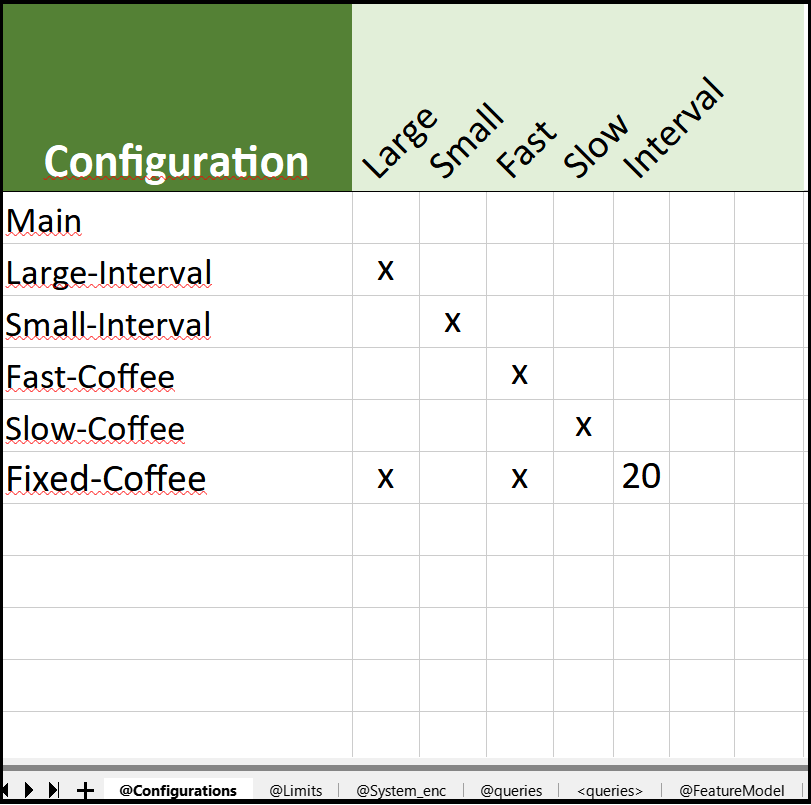
\includegraphics[width=0.8\linewidth]{images/new_example.png}};
            \begin{scope}[x={(image1.south east)},y={(image1.north west)}]
                \draw[black, thick] (0,0) rectangle (1,1); % coordenadas normalizadas
            \end{scope}
        \end{tikzpicture}
        \caption{Configurations Sheet Uppex}
        \label{fig:cof_CM}
    \end{minipage}
\end{figure}

It is necessary to construct the feature model in the corresponding sheet, as shown in Figure \ref{fig:cof_FM}, in order to constrain the feature selections and prevent combinations that do not make sense for the system in question.

\begin{figure}[H]
    \centering
    \begin{minipage}{0.5\textwidth}
        \centering
        \begin{tikzpicture}
            \node[anchor=south west,inner sep=0] (image1) at (0,0) {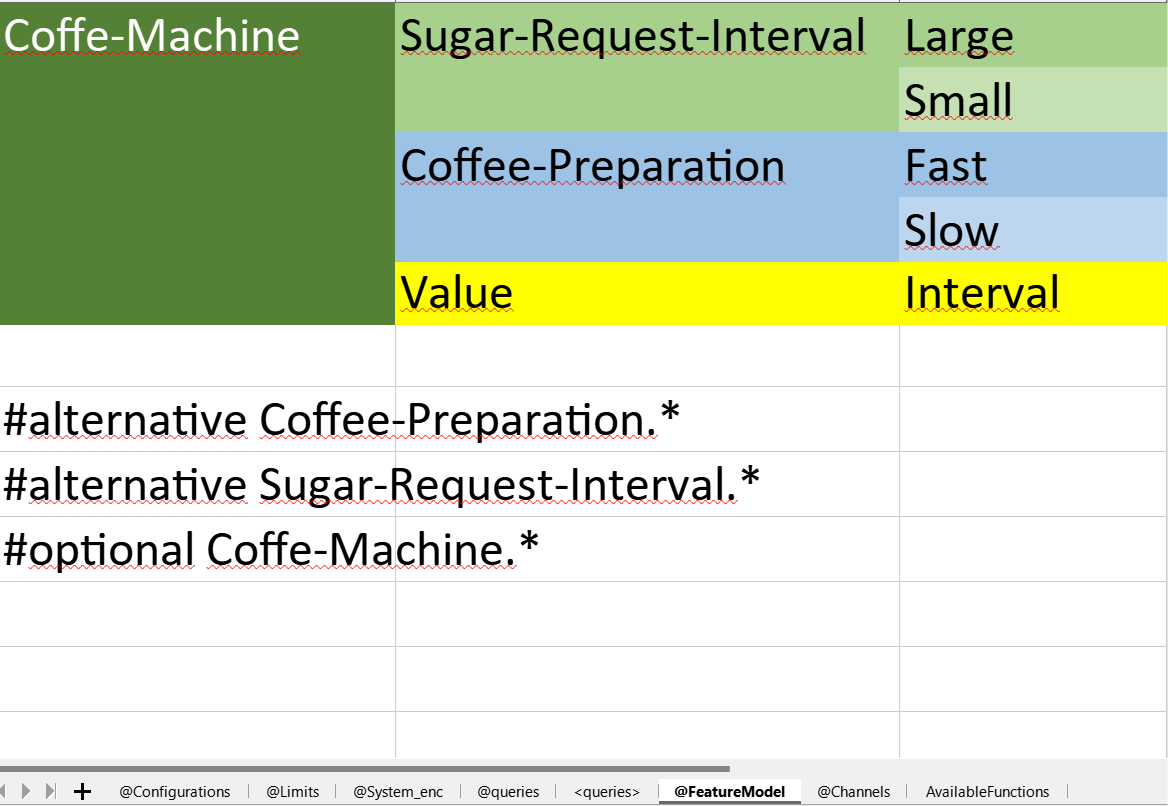
\includegraphics[width=0.8\linewidth]{images/new_FM.png}};
            \begin{scope}[x={(image1.south east)},y={(image1.north west)}]
                \draw[black, thick] (0,0) rectangle (1,1); % coordenadas normalizadas
            \end{scope}
        \end{tikzpicture}
        \caption{Feature Model Sheet Uppex}
        \label{fig:cof_FM}
    \end{minipage}
\end{figure}


We also built the Limits and System\_enc sheets, which represent the constraints applied to each parameter, as shown in Figures \ref{fig:PCSheetCM} and \ref{fig:LSheetsCM}, respectively.



\begin{figure}[H]
    \centering
    \begin{minipage}{0.48\textwidth}
        \centering
        \begin{tikzpicture}
            \node[anchor=south west,inner sep=0] (image1) at (0,0) {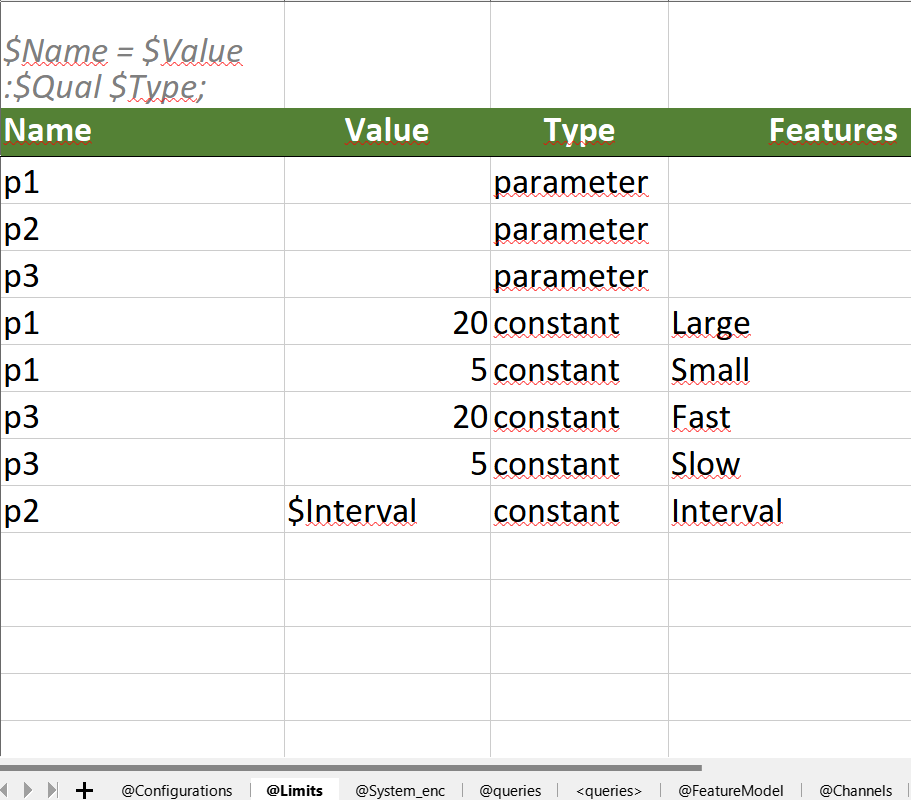
\includegraphics[width=\linewidth]{images/new_Lim.png}};
            \begin{scope}[x={(image1.south east)},y={(image1.north west)}]
                \draw[black, thick] (0,0) rectangle (1,1); % coordenadas normalizadas
            \end{scope}
        \end{tikzpicture}
        \caption{Limits Sheet}
        \label{fig:PCSheetCM}
    \end{minipage}
    \hfill
    \begin{minipage}{0.48\textwidth}
        \centering
        \begin{tikzpicture}
            \node[anchor=south west,inner sep=0] (image2) at (0,0) {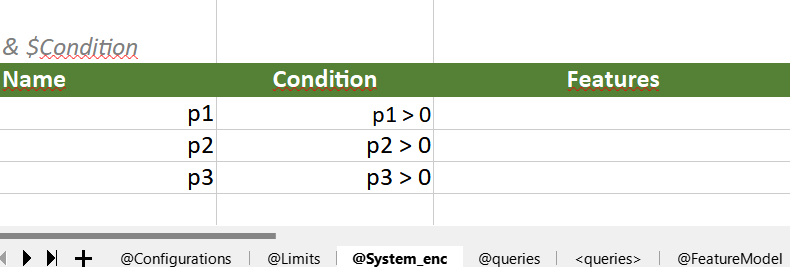
\includegraphics[width=\linewidth]{images/par_new.png}};
            \begin{scope}[x={(image2.south east)},y={(image2.north west)}]
                \draw[black, thick] (0,0) rectangle (1,1); % coordenadas normalizadas
            \end{scope}
        \end{tikzpicture}
        \caption{Parameters Constrain Sheet}
        \label{fig:LSheetsCM}
    \end{minipage}
\end{figure}

Finally, we configured the Queries sheet (Figure \ref{fig:Q_CM}). For the sake of simplicity, all configurations are set to verify the Deadlock property. Additionally, although not shown in the figure, the synthesis mode (as explained in the previous chapter) is set to synth.

\begin{figure}[H]
    \centering
    \begin{minipage}{\textwidth}
        \centering
        \begin{tikzpicture}
            \node[anchor=south west,inner sep=0] (image1) at (0,0) {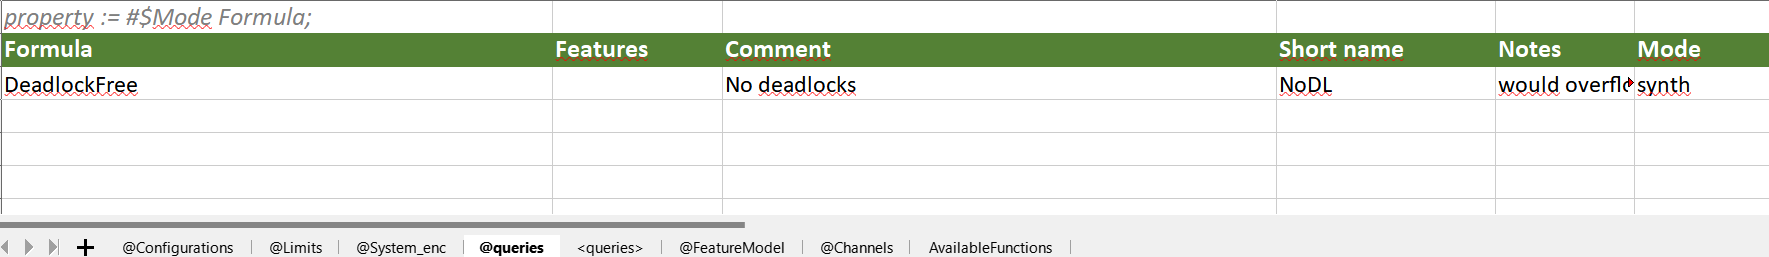
\includegraphics[width=\linewidth]{images/new_d.png}};
            \begin{scope}[x={(image1.south east)},y={(image1.north west)}]
                \draw[black, thick] (0,0) rectangle (1,1); % coordenadas normalizadas
            \end{scope}
        \end{tikzpicture}
        \caption{Queries Sheet Uppex}
        \label{fig:Q_CM}
    \end{minipage}
\end{figure}


With the parameterized model, we can run the JAR file, and the operating mode is exactly the same as the old version. Within the same directory, we need to have the JAR file and we can name it uppex.jar, the Excel file, and the Imitator file, with the last two files needing to have the same name.

In the terminal, we use the command: \texttt{java -jar uppex.jar -runAll Imitator\_Model.imi}, thus compiling all configurations. In each configuration, the deadlock property will be verified, and the results will be presented in an HTML file grouped by property and by configuration. For our example, the results can be found in Appendix C.

%discussion
As expected, for each of the configurations, in order for the property to be satisfied, $p_1$, $p_2$, and $p_3$ must fall within a specific range determined by the algorithm used. It is worth noting that the fixed\_coffee configuration does not have any associated interval since, as previously explained, all its variables are assigned fixed values. This turns it into a parametric model that, for the chosen values, verifies the condition. In this case, it reduces to the model checking of timed automata.

%motivating
% \section{Changes in UPPEX}
\section{Implementation details}
%colcoar intro
As previously mentioned, we will now provide a detailed explanation of the changes made to the old version of the tool to accommodate the new functionalities.
\subsection{Imitator Parser}
%alterar secções abaixo

To properly process and store the data extracted from Uppaal (.xml), Imitator (.imi), and Excel files, two specific data structures need to be created. These structures are designed to organize, structure, and simplify access to the collected information, ensuring efficient storage and data handling.

For reading Uppaal models, there is a base type called \textbf{Block} (like a code block), declared as a trait. Inside each block, there can be a tag (\textbf{NameBl}) that identifies the relevant part of the model, while the rest is called \textbf{content}.For this, two classes are created that extend this type, meaning they inherit its basic properties and behaviors, allowing them to reuse and specialize its functionalities. It is important to note that NameBl is written as an abstract class, meaning it cannot be instantiated directly and serves as a model for other classes that extend it. This means that NamedBl can define common methods and attributes but leaves the implementation of certain details to its subclasses. These are called \textbf{XmlElm}, if the tag is of the XML type, or \textbf{AnnotationBl}, when it is an annotation. Each of these subclasses specializes the behavior defined in the abstract class NamedBl, adapting to the specific type of block they represent. This ensures a clear distinction between XML elements and annotations, allowing proper handling for each case within the model. Along with the data structure, we also have a variety of helper functions aimed at displaying the model. 

In the constructors of the classes \texttt{NamedBl}, \texttt{XmElm}, and \texttt{AnnotationBl}, the following parameters are used:  

\begin{itemize}
    \item \textbf{\texttt{name}}: 
    
    Represents the name of the annotation.
    \item \textbf{\texttt{oldLines}}: 
    
    Contains the original content of the annotation, exactly as it appears in the source file.
    \item \textbf{\texttt{newLines}}: 
    
    Stores the updated content of the annotation, rewritten with the new values of the selected product. These values are formatted according to the structure specified in the first cell of the Excel file that matches both the name and type of the annotation.
\end{itemize}

To demonstrate how it works, we can consider the listing \ref{lst:imitator_example}, as an example. In this case, there is only one block with an annotation, specifically an annotation block of type \textbf{(Name)}, where the name is "Limits", corresponding to the \textbf{name} parameter in the constructor. The content of this block will be stored exactly as it is in the \texttt{oldLines} parameter.

To populate \texttt{newLines}, we need to refer to the Uppex Excel file. The Excel file contains a sheet with the same name as the annotation block, as shown in Figure \ref{fig:sheet}. Additionally, in the first cell of the sheet, we can find the structure that specifies how to construct each annotation block.

For instance, if we consider the product in question to be "lazy," then the annotation block is rewritten according to the structure defined in the Excel file. This rewritten block is displayed in listing \ref{lst:uppaal_example}. The Excel part will be detailed in the next chapter.



\lstdefinelanguage{UPPAAL}
{
    keywords={var, clock, discrete, bool, constant, parameter, automaton, sync, loc, invariant, when, do, goto, end, init},
    keywordstyle=\color{keywordcolor}\bfseries,
    % morecomment=[l]{(*},
    % morecomment=[r]{*)},
    commentstyle=\color{commentcolor}\textit,
    morestring=[b]",
    stringstyle=\color{stringcolor},
    basicstyle=\ttfamily\small,
    backgroundcolor=\color{backgroundcolor},
    tabsize=4,
    showstringspaces=false,
    breaklines=true
}


\definecolor{keywordcolor}{RGB}{0,0,255}      % Azul para palavras-chave
\definecolor{commentcolor}{RGB}{0,128,0}      % Verde para comentários
\definecolor{stringcolor}{RGB}{163,21,21}     % Vermelho escuro para strings
\definecolor{backgroundcolor}{RGB}{240,240,240}

\begin{figure}[H]
    \centering
    \begin{lstlisting}[language=UPPAAL, caption={Example of Imitator syntax}, label={lst:imitator_example},mathescape=true]
var
    session, t : clock;
    nails : discrete;
    b = True : bool;


(* @Limits *)
    sessionTime = 100 : constant;
    countNails = True : bool;
    infiniteNails = False : bool;   $\tikz[overlay, remember picture]{\coordinate(nails);}$
    reactTime = 20 : constant;
    totalNails : parameter;
    \end{lstlisting}
\end{figure}

% Creating arrows and explanations
\begin{tikzpicture}[overlay, remember picture]

Explanation box 1
\node[text width=5cm, draw, fill=white] (box1) at (12, 5.4) {
    \textbf{Annotation Block} \\
   \small Stored as Annotation Block named Limits
};
%%% Variation using the "nails" coordinate
% \node[text width=5cm, draw, fill=white,xshift=60mm] (box1) at (nails) {
%     \textbf{Annotation Block} \\
%    \small Stored as Annotation Block named Limits
% };

% Explanation box 2
\node[text width=5cm, draw, fill=white] (box2) at (12, 8.5) {
    \textbf{Content Block} \\
    \small Stored as Content Block
};

\draw[->, red, thick] (3.5,5.4) -- (box1.west);
% \draw[->, red, thick] (nails) -- (box1);
\draw[->, red, thick] (4.5,8.5) -- (box2.west);

\end{tikzpicture}

\begin{figure} [H]
    \centering
    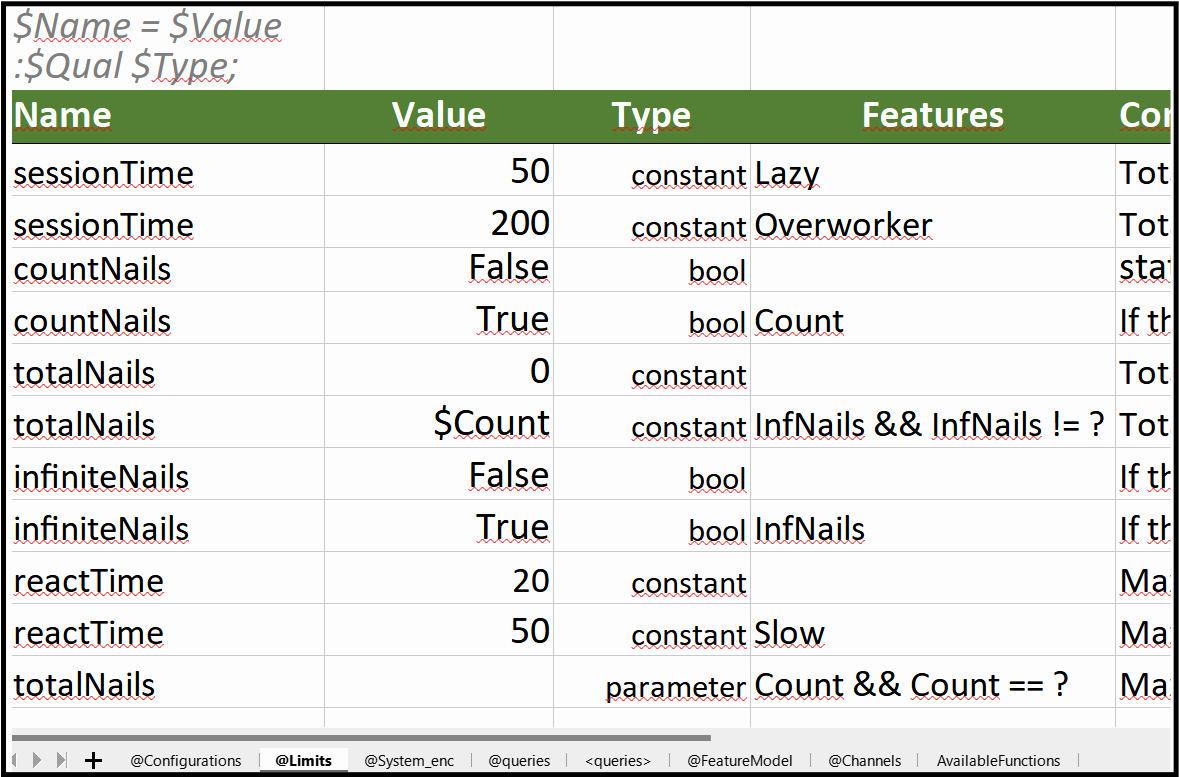
\includegraphics[width=0.75\linewidth]{images/uppex_imi.png}
    \caption{Limits Sheet from Uppex }
    \label{fig:sheet}
\end{figure}

\begin{figure}[H]
    \centering
    \begin{lstlisting}[language=UPPAAL, caption={Annotation Block rewritten with new values}, label={lst:uppaal_example}]
(* @Limits *)
    countNails = False : bool;
    sessionTime = 50 : constant;
    totalNails = 0 : constant;
    infiniteNails = False : bool;
    reactTime = 20 : constant;
    \end{lstlisting}
\end{figure}

%\vspace{1cm}


To better understand the Data structure, we built a class diagram, as shown in Figure \ref{fig:UPDS}. The diagram highlights the trait \textbf{Block}, represented at the top, which serves as the general interface for the different elements of the parser. From this trait, two main branches emerge, represented by arrows pointing downwards. These arrows denote inheritance, meaning that both \textbf{Content} and \textbf{NamedBl} are specializations of the abstract Block type. In other words, they inherit its interface but add their own attributes and behavior. On the right-hand side, the class \textbf{NamedBl} is drawn with a dashed outline and the stereotype <<abstract>>. This indicates that it is an abstract class: it cannot be instantiated directly, but instead serves as a blueprint for more specific subclasses. These subclasses are \textbf{XmlElm} and \textbf{AnnotationBl}, connected to \textbf{NamedBl} by arrows that also denote inheritance. Both subclasses extend the abstract definition of \textbf{NamedBl} by providing concrete realizations that can actually be instantiated. The Content class, on the other hand, directly extends Block without going through \textbf{NamedBl}, as it only stores a simple string attribute. This structure allows Uppaal to organize the parser in a modular way: \textbf{NamedBl} acts as a base definition for all named blocks (whether XML elements or annotations), while Content provides a lightweight alternative for storing raw strings.

\begin{figure}[H]
    \centering
    % \begin{standalone}
        \begin{tikzpicture}[node distance=2.5cm, auto]
          % Nó para Block (sealed trait)
          \node (block) [trait,fill=red!10]
          {\begin{tabular}{c}
          <<trait>>\\
           \textbf{Block}
           \end{tabular}};
        % 
        % 
          % Nó para Content (classe concreta)
          \node (content) [class,fill=red!10, below left=of block]
          { \begin{tabular}{c}
            \textbf{Content} \\[1ex]\hline
            c: String
          \end{tabular}};
        % 
          % Nó para NamedBl (sealed abstract class)
          \node (namedbl) [abstractclass,fill=red!10, below right=1cm of block,text width=5cm, align=center]
          {\begin{tabular}{c}
            <<abstract>>\\
           \textbf{NamedBl}  ~\\\hline
           name: String \\ 
           oldLines: Lines \\ 
           newLines: Lines ~\\ \hline
           prettyName: String
           \end{tabular}};
        % 
          % Nó para AnnotationBl (classe concreta)
          \node (annotationbl) [class,fill=red!10, below=1.5cm of namedbl]
          {\begin{tabular}{c}\textbf{AnnotationBl} ~\\ \hline
           n: String \\ 
           oldL: Lines \\ 
           newL: Lines
           \end{tabular}};
        % 
          % Nó para XmlElm (classe concreta)
          \node (xmlelm) [class,fill=red!10, left=of annotationbl]
          {\begin{tabular}{c}\textbf{XmlElm} ~\\ \hline 
           n: String \\ 
           oldL: Lines \\ 
           newL: Lines
           \end{tabular}};
        % 
        % 
          % Conexões (relações de herança/implementação)
          %\draw [arrow] (Model) -- (GenModel);
          \draw [arrow] (content) -- (block);
          \draw [arrow] (namedbl) -- (block);
          \draw [arrow] (annotationbl) -- (namedbl);
          \draw [arrow] (xmlelm) -- (namedbl);
        \end{tikzpicture}
    % \end{standalone}
    \caption{Uppaal Parser Data Structure}
    \label{fig:UPDS}
\end{figure}

The data structure for Imitator will be very similar, allowing us to reuse the Uppaal structure. However, we can omit the XmlElm blocks, as they are no longer applicable, as shown in Figure \ref{fig:IPDS}.

\begin{figure}[H]
    \centering
    % \begin{standalone}
        \begin{tikzpicture}[node distance=2.5cm, auto]
          % Nó para Block (sealed trait)
          \node (block) [trait,fill=red!10]
          {\begin{tabular}{c}
          <<trait>>\\
           \textbf{Block}
           \end{tabular}};
        % 
        % 
          % Nó para Content (classe concreta)
          \node (content) [class,fill=red!10, below left=of block]
          {\begin{tabular}{c}\textbf{Content} \\[3mm] \hline
           c: String
           \end{tabular}};
        % 
          % Nó para NamedBl (sealed abstract class)
          \node (namedbl) [abstractclass,fill=red!10, below right=1cm of block,text width=4.5cm]
          {\begin{tabular}{c}<<abstract>>\\
           \textbf{NamedBl} \\ \hline
           name: String \\ 
           oldLines: Lines \\ 
           newLines: Lines \\ \hline
           prettyName: String
           \end{tabular}};
        
          % Nó para AnnotationBl (classe concreta)
          \node (annotationbl) [class,fill=red!10, below=1.5cm of namedbl]
          {\begin{tabular}{c}\textbf{AnnotationBl}\\ \hline
           n: String \\ 
           oldL: Lines \\ 
           newL: Lines
           \end{tabular}};
% 
                % 
          % Conexões (relações de herança/implementação)
          %\draw [arrow] (Model) -- (GenModel);
          \draw [arrow] (content) -- (block);
          \draw [arrow] (namedbl) -- (block);
          \draw [arrow] (annotationbl) -- (namedbl);
        \end{tikzpicture}
    % \end{standalone}
    \caption{Imitator Parser Data Structure}
    \label{fig:IPDS}
\end{figure}


To expand the tool to support Imitator models while reusing code without adding unnecessary complexity(such as code duplication and the need to assign different names to identical code blocks), a trait with several abstract methods has been created. The functions responsible for rewriting code blocks that were previously defined only for UPPAAL will be implemented in the Imitator or Uppaal classes, which extend the trait. This will allow code reuse while maintaining the flexibility and modularity of the system.
This structure will also be reused, although, in the case of Imitator, the XmlElm block will not be used, as the tags inside < > will not be employed. This structure will now be part of a new singleton called GenModel and it is imported during the parsing of either the Uppaal or Imitator file, with the trait class also being declared in the same file and having the same name.



With the data structure set up, we need to build a parser to read the Imitator file, classifying each part according to the tags encountered. In parsing, code is taken from the preprocessor, broken into smaller pieces and analyzed so other software can understand it. The parser does this by building a data structure out of the pieces of input \cite{techtarget_parser}. 

Note that in the new version of Uppex, the notation that identifies the beginning of an annotation block for Imitator is in the form "$\textbf{(*Name of the Annotation Block*)}$".%, while the XML block remains the same as "\textbf{<Name of the XML Annotation Block>}". However, in the case of Imitator, the latter will not be used.


\newcolumntype{L}{>{\ttfamily}l}

\begin{table}[h]
    \centering
    \begin{tcolorbox}[colback=gray!10, colframe=black]
    \caption{Syntactic rules of the grammar}
    \label{tab:syntactic-rules_fin}
    \begin{tabular}{L L L}
        \textbf{Rule} & \textbf{::=} & \textbf{Definition} \\
        \hline
        annotationBlock & ::= & "(*" "@" anName "*)" [ newLine body ] \\
        lineBlock & ::= & line \\
        body & ::= & repsep(neLine, newLine) \\
    \end{tabular}
    \end{tcolorbox}
\end{table}

\begin{table}[H]
    \centering
    \begin{tcolorbox}[colback=gray!10, colframe=black]
    \caption{Basic tokens of the grammar}
    \label{tab:basic-tokens_fin}
    \begin{tabular}{L L L}
        \textbf{Token} & \textbf{::=} & \textbf{Definition} \\
        \hline
        newLine & ::= & \verb|\n| \\
        line & ::= & rep(word) \\
        neLine & ::= & rep1(word) \\
        word & ::= & \verb|[^\n]+| \\
        anName & ::= & \verb|[^*]+| \\
    \end{tabular}
    \end{tcolorbox}
\end{table}

The functioning of this parser is quite simple. We start by reading the file as a string and passing the result to the parse function, which in turn calls imitator, the main parser that splits the code into blocks. The syntactic rules used for this parsing process are shown in Table \ref{tab:syntactic-rules_fin}, while the basic tokens of the grammar are presented in Table \ref{tab:basic-tokens_fin}. The parser uses repsep(imitatorElem, newLine) to divide the content into lines or blocks. imitatorElem works as a block recognizer: if it finds (*@name*), it identifies it as an annotation(Annotation Block) and stores its name and content; otherwise, it considers the line as normal content (Content).

%\definecolor{keywordcolor}{rgb}{0.5,0.0,0.5}
%\definecolor{commentcolor}{rgb}{0.25,0.5,0.35}
%\definecolor{stringcolor}{rgb}{0.58,0.0,0.0}
%\definecolor{backgroundcolor}{rgb}{0.95,0.95,0.95}



%\begin{figure}[H]
%    \centering
%    \begin{standalone}
%        \begin{tikzpicture}[node distance=0.5cm, auto]
%            % Nó para GenModel (trait)
%          \node (GenModel) [trait,fill=green!10,text width=5cm] {
%          \centering <<trait>>\\
%          \centering \textit{\textbf{GenModel}} 
%%          \\[1ex] \\ \hline \\[1ex]
%          blocks: List[Block] \\[1ex] \\ \hline \\[1ex]
%          toString: String \\[1ex]
%          \textit{buildold} : \textit{String}  \\[1ex]
%          \textit{buildnew} : \textit{String}  \\[1ex]
%          \textit{build} : \textit{String}
%        };
        
        

%           \node (Imitator) [class,fill=green!10,text width=5cm,below left=of GenModel] {
%          \centering <<abstract>>\\
%          \centering \textit{\textbf{Imitator}} 
%          \\[1ex] \\ \hline \\[1ex]
%          blocks: List[Block] \\[1ex] \\ \hline \\[1ex]
%          toString: String \\[1ex]
%          buildold : String  \\[1ex]
%          buildnew : String  \\[1ex]
%          build : String
%        };

%        \node (Uppaal) [class,fill=green!10,text width=5cm,below right=of GenModel] {
%          \centering <<abstract>>\\
%          \centering \textit{\textbf{Uppaal}} 
%          \\[1ex] \\ \hline \\[1ex]
%          blocks: List[Block] \\[1ex] \\ \hline \\[1ex]
%          toString: String \\[1ex]
%          buildold : String  \\[1ex]
%          buildnew : String  \\[1ex]
%          build : String
%        };
        
           
 %           \draw [arrow] (Uppaal) -- (GenModel);
 %           \draw [arrow] (Imitator) -- (GenModel);
  %      \end{tikzpicture}
  %  \end{standalone}
  %  \caption{Caption}
  %  \label{fig:enter-label}
%\end{figure}


%\tikzstyle{class} = [rectangle, draw, rounded corners, text width=4cm, minimum height=2em, align=left, font=\ttfamily, fill=blue!10]
%\tikzstyle{abstractclass} = [class, fill=green!10, dashed]
%\tikzstyle{trait} = [class, fill=green!10]
%\tikzstyle{arrow} = [thick,->,>=stealth]


%\begin{center}
%\begin{tikzpicture}[node distance=2.5cm, auto]
    % Nó para GenModel (trait)
%  \node (GenModel) [trait,yshift=-99cm,text width=5cm] {
%  \centering <<trait>>\\
%  \centering \textbf{GenModel} 
%  \\[1ex] \\ \hline \\[1ex]
%  blocks: List[Block] \\[1ex] \\ \hline \\[1ex]
%  toString: String
%5};

  % Nó para Model (classe concreta)
%  \node (Model) [class,fill=green!10,left=of GenModel]
%  {\centering \textbf{Model} \\[1ex] \\ \hline \\[1ex]
%   \\
%   bs: List[Block]};

   
%    \draw [arrow] (Model) -- (GenModel);
%\end{tikzpicture}
%\end{center}

\subsection{Better feature expressions in the Excel Reader}

%explicar as features expressions e o seu uso

Regarding the Excel file, its functionality has remained largely the same, with changes limited to the Feature Model.

In the previous version, each annotation table mapped variables to patterns and included a special Features column containing boolean expressions over feature names. Entries were included only if the expression evaluated to true under the selected configuration. If multiple entries shared the same key, the last one would override the previous ones. This behavior is preserved in the new model. However, with the enhanced capabilities of the new backend, the type of supported boolean expressions had to be extended. In addition to checking for active configurations, it is now possible to compare features with strings and doubles, allowing the definition of richer and more expressive configurations, as illustrated by some examples in Table \ref{tab:bass}.

\begin{table}[H]
\centering
\begin{tabular}{@{}cll@{}}
\hline
\textbf{Expression Type} & \textbf{Old Version} & \textbf{New Version} \\
\hline
Simple Boolean Expressions & \texttt{Lazy \&\& !Overworker} & \texttt{Lazy \&\& !Overworker} \\
\hline
Comparison with Strings & \textcolor{gray}{Not Supported} & \texttt{Count == ?} \\
\hline
Comparison with Numbers & \textcolor{gray}{Not Supported} & \texttt{Slow > 0.5} \\
\hline
Combination of Types & \textcolor{gray}{Not Supported} & \texttt{(Count == ?) \&\& (Slow < 10)} \\
\hline
\end{tabular}
\caption{Evolution of Boolean Expression Support in the \texttt{Features} Field}
\label{tab:bass}
\end{table}

The first step was to update the syntactic structure of the logical expressions that the parser can analyze and evaluate, referred to as FeatExpr. This structure is represented by an enum, which is a data type that represents a fixed and limited set of possible values. In Scala, enums can be used similarly to sealed traits with case classes, allowing for the clear definition of immutable and extensible data hierarchies. In this new syntactic structure, the Comp value was introduced, as shown in Figure \ref{fig:FeatExpr}.


\begin{figure}[H]
\centering
\begin{minipage}{0.9\linewidth}
\begin{verbatim}
    enum FeatExpr:
      case Feature(id: String)
      case And(f1: FeatExpr, f2: FeatExpr)
      case Or(f1: FeatExpr, f2: FeatExpr)
      case Imply(f1: FeatExpr, f2: FeatExpr)
      case Not(f: FeatExpr)
      case Comp(v1: FeatVal, v2: FeatVal, op: String)
      case True
\end{verbatim}
\end{minipage}
\caption{Updated FeatExpr Enum}
\label{fig:FeatExpr}
\end{figure}

The Comp value takes three arguments: v1 and v2 of type FeatVal, and a third one called op, which indicates the type of operator that we want to use. FeatVal is a new data structure (as shown in Figure \ref{fig:FeatVal}) created to represent the possible values that the elements on each side of the comparison can take, which are:

\begin{itemize}
  \item \texttt{Feature(id: String)}: a reference to a feature, that is, a variable whose value will be looked up in the product.
  \item \texttt{Value(n: Double)}: a numeric literal value.
  \item \texttt{Opt(o: String)}: an option, such as a list of categories, states, or labels.
\end{itemize}

\begin{figure}[H]
\centering
\begin{minipage}{0.9\linewidth}
\begin{verbatim}
    enum FeatVal:
      case Feature(id:String)
      case Value(n:Double)
      case Opt(o:String)
\end{verbatim}
\end{minipage}
\caption{FeatVal Enum}
\label{fig:FeatVal}
\end{figure}

It was also necessary to update the function responsible for evaluating a logical expression of type FeatExpr (as shown in Figure \ref{fig:Eval}), based on a set of features provided in FProd, which represents a product configuration (e.g., a Map[String, Any] containing the names and values of the features).


\begin{figure}[H]
\centering
\begin{minipage}{0.9\linewidth}
\begin{verbatim}
    def eval(fe: FeatExpr)(using prod: FProd): Boolean = fe match
      case Feature(id) => prod contains id
      case And(f1,f2) => eval(f1) && eval(f2)
      case Or(f1,f2) => eval(f1) || eval(f2)
      case Imply(f1, f2) => !eval(f1) || eval(f2)
      case Not(f2) => !eval(f2)
      case Comp(v1,v2,op) => getResult(Comp(v1,v2,op))
      case True => true
\end{verbatim}
\end{minipage}
\caption{Updated Eval Function}
\label{fig:Eval}
\end{figure}

As a result of the changes made to the definition of FeatExpr, a new case named Comp was added, representing a comparison between two elements. When an expression of this type is evaluated, a helper function, getResult, is called. This function applies the logical operation represented by op between the operands v1 and v2. It determines the type of the values and executes the corresponding operation—such as equality, inequality, greater than, or less than—returning a Boolean value as intended.

Finally, it is necessary to update the parser so that it can correctly identify and capture comparison expressions whenever they appear in the Feature column of the Annotations tables in the Excel file. As shown in Table \ref{tab:s}, the featComp rule was introduced, allowing the parsing of comparisons between two elements. This rule, on the left-hand side of the expression, captures a featureVal representing a feature, the operator (op) which must be one of the supported comparison operators, and finally, featValOpt, which can be a number, a list, or text, as shown in Table \ref{tab:e}.



\begin{table}[H]
\centering
\begin{tabular}{r@{\texttt{ ::= }}l}
\hline
\multicolumn{1}{c}{\textbf{Rule}} & \textbf{Definition} \\
\hline
\texttt{featExpr}     & \texttt{featImpl} ~$\mid$~ $\varepsilon$ \\
\texttt{featImpl}     & \texttt{featDisj} \ [ (``\texttt{->}'' $\mid$ "\texttt{=>}" $\mid$ "\texttt{<->}" $\mid$ "\texttt{<=>}" $\mid$ "\texttt{\#}") \ \texttt{featImpl} ] \\
\texttt{featDisj}     & \texttt{featConj} \ [ ``\texttt{||}'' \ \texttt{featDisj} ] \\
\texttt{featConj}     & \texttt{literal} \ [ ``\texttt{\&\&}'' \ \texttt{featConj} ] \\
\texttt{literal}      & ``\texttt{(}'' \ \texttt{featImpl} \ ``\texttt{)}'' \\
\multicolumn{1}{c}{}  & $\mid$ "\texttt{!}" \ \texttt{literal} \\
\multicolumn{1}{c}{}  & $\mid$ "\texttt{true}" \\
\multicolumn{1}{c}{}  & $\mid$ "\texttt{false}" \\
\multicolumn{1}{c}{}  & $\mid$ \texttt{featComp} \\
\multicolumn{1}{c}{}  & $\mid$ \texttt{feature} \\
\texttt{featComp}     & \texttt{featureVal} \ (``\texttt{<}'' $\mid$ "\texttt{>}" $\mid$ "\texttt{<=}" $\mid$ "\texttt{>=}" $\mid$ "\texttt{==}" $\mid$ "\texttt{!=}") \ \texttt{featValOpt} \\
\texttt{feature}      & \textit{identifier} \\
\texttt{featureVal}   & \textit{identifier} \\
\texttt{featValOpt}   & \textit{number} $\mid$ "\texttt{[} \textit{optionList} \texttt{]}" $\mid$ \textit{optText} \\
\hline
\end{tabular}
\caption{Syntactic rules of the feature expression grammar}
\label{tab:s}
\end{table}


\begin{table}[H]
\centering
\begin{tabular}{rl}
\hline
\textbf{Token} & \textbf{::= Definition} \\
\hline
identifier  & \texttt{[a-zA-Z0-9\_][a-zA-Z0-9\-\_]*} \\
number      & \texttt{[0-9]+(\textbackslash.[0-9]+)?} \\
optionList  & \texttt{[a-zA-Z\_,-]+} \\
optText     & \texttt{[\textbackslash??,a-zA-Z\_,-]+} \\
\hline
\end{tabular}
\caption{Basic tokens of the feature expression grammar}
\label{tab:e}
\end{table}


\subsection{Report generation}

As previously mentioned, Uppex returns an HTML report summarising the configurations and the corresponding verified properties, along with their results — True if the property holds, or False otherwise. The report is implemented as a class with the same name, Report, which includes attributes and methods to:

\begin{itemize}
    \item Add Products

    \item Add results to the last added product (OK, Fail, Timeout).
\end{itemize}

This data structure is defined as:

\[
\texttt{Map[String, Map[String, Set[String]]]}
\]

That is:

\[
\text{Product} \rightarrow \{\text{"ok"} \rightarrow \text{Set[Property]}, \ \text{"fail"} \rightarrow \text{Set[Property]}, \ \text{"timeout"} \rightarrow \text{Set[Property]}\}\}
\]

With the introduction of the new backend and the addition of parametric models, it was necessary to implement a function to add the parametric constraints, called addConstraint.

\[
\hspace{-1cm}
\text{Product} \rightarrow \{\text{"ok"} \rightarrow \text{Set[Property]}, \ \text{"fail"} \rightarrow \text{Set[Property]}, \ \text{"timeout"} \rightarrow \text{Set[Property]}\}, \ \text{"constrain"} \rightarrow \text{Set[Property]}\}\}
\]

In addition, with the possibility of generating an image from the model, the addImage function was included, which allows associating the model images with the configurations. The structure is quite simple, consisting of a map of the configuration and the location where the model image is stored, if it exists.


\[
\texttt{Map[String, Set[String]]}
\]

That is:

\[
\text{Product} \rightarrow \text{Set[Images]}
\]

With all the information stored, the class also has a method that compiles this data into the final report. This method iterates through the data structures and aggregates the following into the three sections in which the report is structured:

\begin{itemize}
    \item By Products

    The properties are grouped by products, with different formatting depending on whether they hold, do not hold, or have a parametric interval.

    \item By Property

    The grouping is done by property, with each product having a property according to the result of the respective property.

    \item Image By Product

    In this section, each product is assigned the visual format of the system.
\end{itemize}


\subsection{Imitator Backend}

Finally, it was necessary to implement a new backend, responsible for processing each configuration along with its properties, handling the obtained results, and generating the corresponding report.

As mentioned in the previous chapter, in the Bash terminal, a volume (local folder) will be mounted into the Docker container to allow IMITATOR to run with direct access to the files stored there. The backend assumes that this folder already exists; however, if it does not, it will be automatically created on the desktop with the name examples. This functionality is designed to work correctly on Windows, Linux, and macOS operating systems.

Similarly, for embedding images into the report, a folder named "images" must exist in the same directory as the JAR file. The same logic applies: if the folder does not exist, it will be created automatically.

We can divide the \textbf{Core of the Backend} into two main parts:

\begin{itemize}
    \item \textbf{Function to store the properties to be verified:} This function aims to generate, for each property defined in the configurations, a separate file with the extension \texttt{.imipop}. Each file contains the property syntax exactly as specified in the Excel file and will later be verified against the model. These files are stored in a specific directory named \texttt{examples} by default, which is then mounted into the Docker container.

    \item \textbf{Function to run IMITATOR:} This function is responsible for executing IMITATOR inside a Docker container for each of the properties stored in the \texttt{examples} directory. It also checks whether the main \texttt{.imi} model file—with parameters, variables, and constraints updated according to the configuration—exists in that same directory. The function handles the individual execution of each property, interprets the returned results (e.g., \texttt{True}, \texttt{False}, or parametric constraints), and integrates the outcomes into the final report. Additionally, the function generates images of the models to be included in the final report; these images are stored in the \texttt{images} directory, located alongside the \texttt{.jar} file.
\end{itemize}

If the result is \texttt{True} or \texttt{False}, it is added to the report by invoking the \texttt{addOk} or \texttt{addFail} function, respectively. In the case of a parametric constraint, the newly mentioned function \texttt{addConstrain} is called, receiving the constraint as its argument.

We can summarize the process as follows:

\begin{enumerate}
    \item \textbf{Creation of working directories:} Initially, the backend checks whether the required folders (\texttt{examples}, \texttt{images}, and \texttt{volume}) exist in the file system. If they do not, they are created automatically, ensuring compatibility across different operating systems (Windows, Linux, macOS).

    \item \textbf{Generation of the updated model:} Based on the configurations provided by the user, the main model (\texttt{.imi}) is updated with the relevant parameters, variables, and constraints. This model is temporarily saved and will be used in all subsequent verifications.

    \item \textbf{Creation of property files (\texttt{.imiprop}):} For each property specified in the configurations, a separate file with the \texttt{.imiprop} extension is created. These files contain the logical specification of the property to be verified. Each file is stored in the volume folder that will be mounted into the Docker container.

    \item \textbf{Execution of IMITATOR:} The IMITATOR verifier is executed inside a Docker container. For each \texttt{.imiprop} file, the backend invokes IMITATOR with the \texttt{.imi} model and the corresponding property, using the mounted volume containing the generated files. The system waits for the response and interprets the obtained result.

    \item \textbf{Result handling:} Depending on IMITATOR’s response (\texttt{True}, \texttt{False}, or a parametric formula), the result is classified as verified, not verified, or conditional. Additional information such as the type of approximation and execution time may also be recorded.

    \item \textbf{Generation of the final report:} The results of each verification are compiled into a formatted report, with the option to include images of the analyzed models. These images are stored in the \texttt{images} folder and referenced in the report to enhance visualization and interpretation of the results.
\end{enumerate}



\section{Revisiting the Worker and Hammer example}

%alterar texto

For the implementation of the new Uppex, the Coffe Machine and  Worker and Hammer system was selected. 


Starting with the Configuration sheet, the settings from the previous model were kept, and two new configurations were added. This allows for two groups—one non-parametric and the other parametric—in order to demonstrate the versatility of the tool.


\begin{figure}[H]
    \centering
    \begin{minipage}{0.48\textwidth}
        \centering
        \begin{tikzpicture}
            \node[anchor=south west,inner sep=0] (image1) at (0,0) {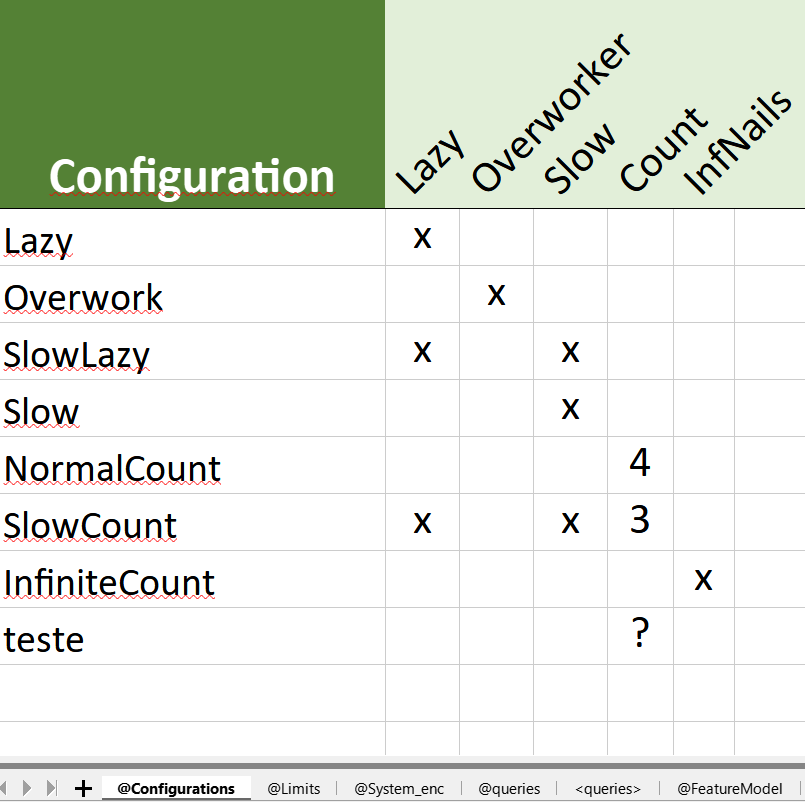
\includegraphics[width=0.8\linewidth]{images/newUp.png}};
            \begin{scope}[x={(image1.south east)},y={(image1.north west)}]
                \draw[black, thick] (0,0) rectangle (1,1); % coordenadas normalizadas
            \end{scope}
        \end{tikzpicture}
        \caption{Configurations Sheet Uppex}
        \label{fig:cof_WH}
    \end{minipage}
\end{figure}

As we can see in Figure \ref{fig:cof_WH}, the test configuration is a parametric configuration, with a ? in the product Count indicating its parametric nature. This can be interpreted as an uncertain or variable number selected for the Count product, unlike the previous configurations which have exact values.


\begin{figure}[H]
    \centering
    \begin{minipage}{0.48\textwidth}
        \centering
        \begin{tikzpicture}
            \node[anchor=south west,inner sep=0] (image1) at (0,0) {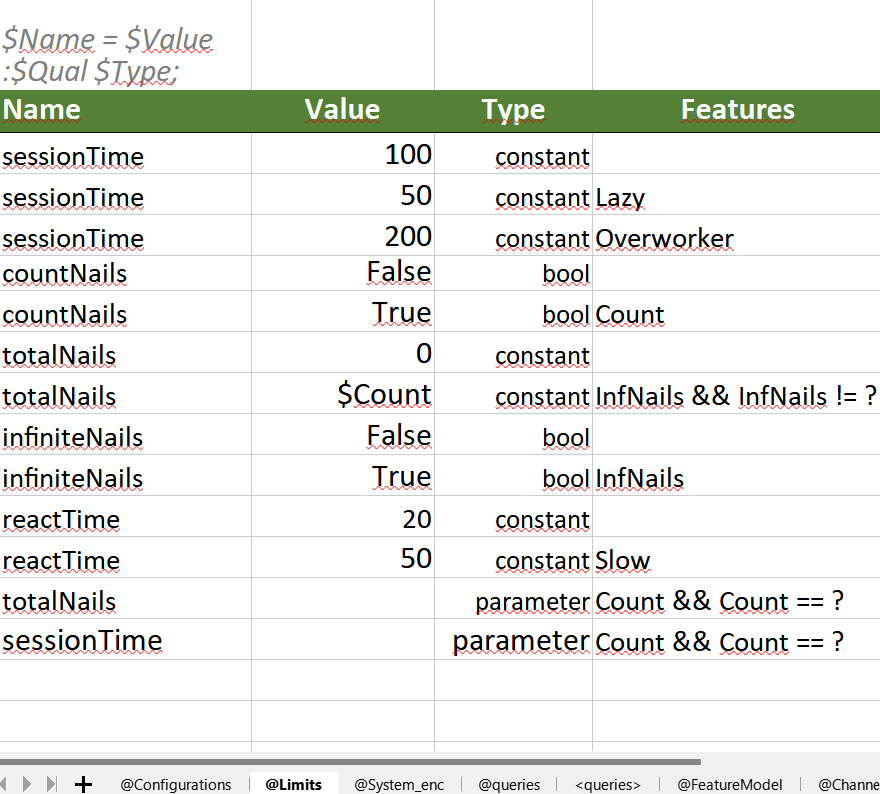
\includegraphics[width=\linewidth]{images/new_limits.png}};
            \begin{scope}[x={(image1.south east)},y={(image1.north west)}]
                \draw[black, thick] (0,0) rectangle (1,1); % coordenadas normalizadas
            \end{scope}
        \end{tikzpicture}
        \caption{Limits Sheet}
        \label{fig:PCSheet}
    \end{minipage}
    \hfill
    \begin{minipage}{0.48\textwidth}
        \centering
        \begin{tikzpicture}
            \node[anchor=south west,inner sep=0] (image2) at (0,0) {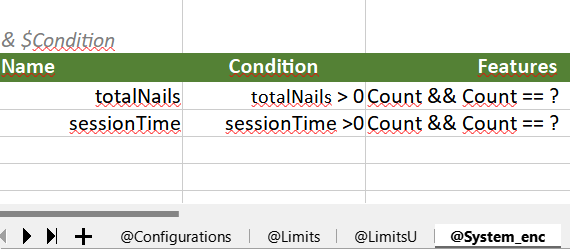
\includegraphics[width=\linewidth]{images/another_par.png}};
            \begin{scope}[x={(image2.south east)},y={(image2.north west)}]
                \draw[black, thick] (0,0) rectangle (1,1); % coordenadas normalizadas
            \end{scope}
        \end{tikzpicture}
        \caption{Parameters Constrain Sheet}
        \label{fig:LSheets}
    \end{minipage}
\end{figure}

In the test configuration, sessionTime and totalNails are introduced as parameters, as shown in Figure \ref{fig:PCSheet}, and the only condition imposed on these parameters is that they must be greater than 0, as seen in Figure \ref{fig:LSheets}. Additionally, the variable declaration pattern has changed compared to the previous version to accommodate the Imitator syntax.

Regarding the Queries Sheet Figure \ref{fig:cof_q}, in the non-parametric configurations that include the Lazy product, we check for the occurrence of deadlock. In the test configuration, in addition to this, we also verify the minimum value of the parameter totalNails required for the Work location in Worker to be reachable. Finally, the parameters constraint is checked to ensure that the NailDone location in Worker is reachable.


\begin{figure}[H]
    \centering
    \begin{minipage}{\textwidth}
        \centering
        \begin{tikzpicture}
            \node[anchor=south west,inner sep=0] (image1) at (0,0) {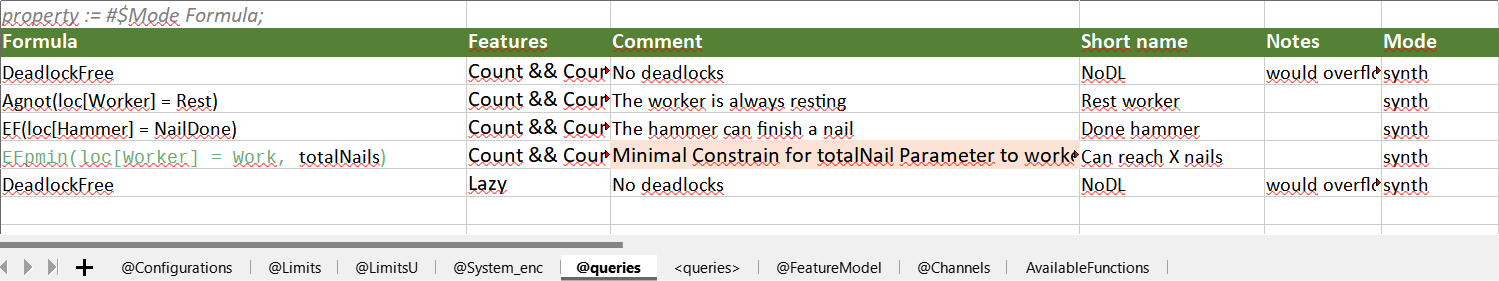
\includegraphics[width=\linewidth]{images/bla.png}};
            \begin{scope}[x={(image1.south east)},y={(image1.north west)}]
                \draw[black, thick] (0,0) rectangle (1,1); % coordenadas normalizadas
            \end{scope}
        \end{tikzpicture}
        \caption{Queries Sheet Uppex}
        \label{fig:cof_q}
    \end{minipage}
\end{figure}

With the updated Excel file, we move on to the parameterization of the .imi file that encapsulates our model. As previously explained, the annotation blocks are identified by the format \texttt{(*Name*)}. In this case, we will have two blocks: one for the variables, named \texttt{(*Limits*)}, and another for the parameter constraints, named \texttt{(*System\_enc*)}. For the non-parametric configurations, the Limits block will have the following structure:

\begin{verbatim}
    (*@Limits*)
    sessionTime = 100
    : constant;
    totalNails = 0
    : constant;
    countNails = True
    : bool;
    reactTime = 20
    : constant;
    infiniteNails = True
    : bool;
\end{verbatim}

Whereas in the test configuration, its content will differ due to the transformation of sessionTime and totalNails into parameters:

\begin{verbatim}
    (*@Limits*)
    countNails = True
    : bool;
    infiniteNails = False
    : bool;
    reactTime = 20
    : constant;
    sessionTime
    : parameter;
    totalNails
    : parameter;
\end{verbatim}


In the terminal, we use the command: \texttt{java -jar uppex.jar -runAll Imitator\_Model.imi}, thus compiling all configurations. The results can be seen in Appendix D. As previously explained, the groupby product and groupby requirement sections maintain the same format as the previous version; however, there is now a new type of result—specifically, the parametric interval, with an indication if an approximation has occurred. Finally, the new section includes the model image for each configuration, except for those not referenced in the queries sheet—that is, in the example, InfiniteCount, Main, NormalCount, Slow, and OverWork will remain empty.






















% !TeX root = ../dissertation.tex

\chapter{Towards a Graphical User Interface for Uppex}

To enhance usability and accessibility, an initial web interface for Uppex was developed, aiming to simplify interaction with the tool and reduce reliance on command-line execution. This interface combines Python (Flask library) on the backend and JavaScript on the frontend to provide a responsive and user-friendly experience. In order to make Uppex a more user-friendly tool for all types of users, initial steps were taken to develop an interface using Python (Flask library) and JavaScript. The proposed frontend was implemented in Python using the Flask library, providing a web-based interface for the uppex.jar verification tool. The application defines routes that enable the loading of model files (XML/IMI), the automatic extraction of configuration parameters from an associated Excel file, and the execution of the different operating modes supported by uppex.jar (--run, --runAll, --validate, --info). The results are then presented directly in the browser, allowing users to interact with the verification engine through an intuitive graphical interface. This approach eliminates the need for command-line interaction, thereby improving usability and reducing the likelihood of user errors.
\medskip

\noindent
\textbf{Requirements.} To be able to use the beta version of the tool, it is necessary to ensure that the following conditions are met: Python, the Java Virtual Machine (JVM), and Bash are installed, and Docker is available.

\medskip

\noindent
\textbf{Installation.} When the conditions above are met, the user can install this GUI by downloading and running the following Bash script:
\url{https://github.com/alexandre04032000/uppex-imitator/blob/Uppex-Imitator/interface.sh}. 
If the process runs successfully, the application will be available on port 8080 of the localhost.

The installation script is designed to automate all necessary steps, including dependency checks, environment setup, and configuration of the server to run the GUI. Users should ensure that they have sufficient permissions to execute Bash scripts and that their system meets the minimum requirements for running the application. After execution, the script will provide output messages indicating the status of each step, such as downloading necessary libraries, setting environment variables, and starting the local server. Once the server is running, users can open a web browser and navigate to \texttt{http://localhost:8080}
 to access the interface.

\medskip

\noindent
\textbf{Running.} This interface allows users to choose between the desired model checker, specifically between Uppaal and IMITATOR. Once one of these options is selected, a menu is displayed (as shown in Figure \ref{fig:UI}), allowing the user to choose from the following options:

\begin{itemize}
    \item Validate the Model
    \item Run a Single Product
    \item Run All Products
    \item Change the Excel File
    \item Change .imi or .xml file
\end{itemize}

\begin{figure}[H]
    \centering
    \begin{minipage}{0.78\textwidth}
        \centering
        \begin{tikzpicture}
            \node[anchor=south west,inner sep=0] (image1) at (0,0) {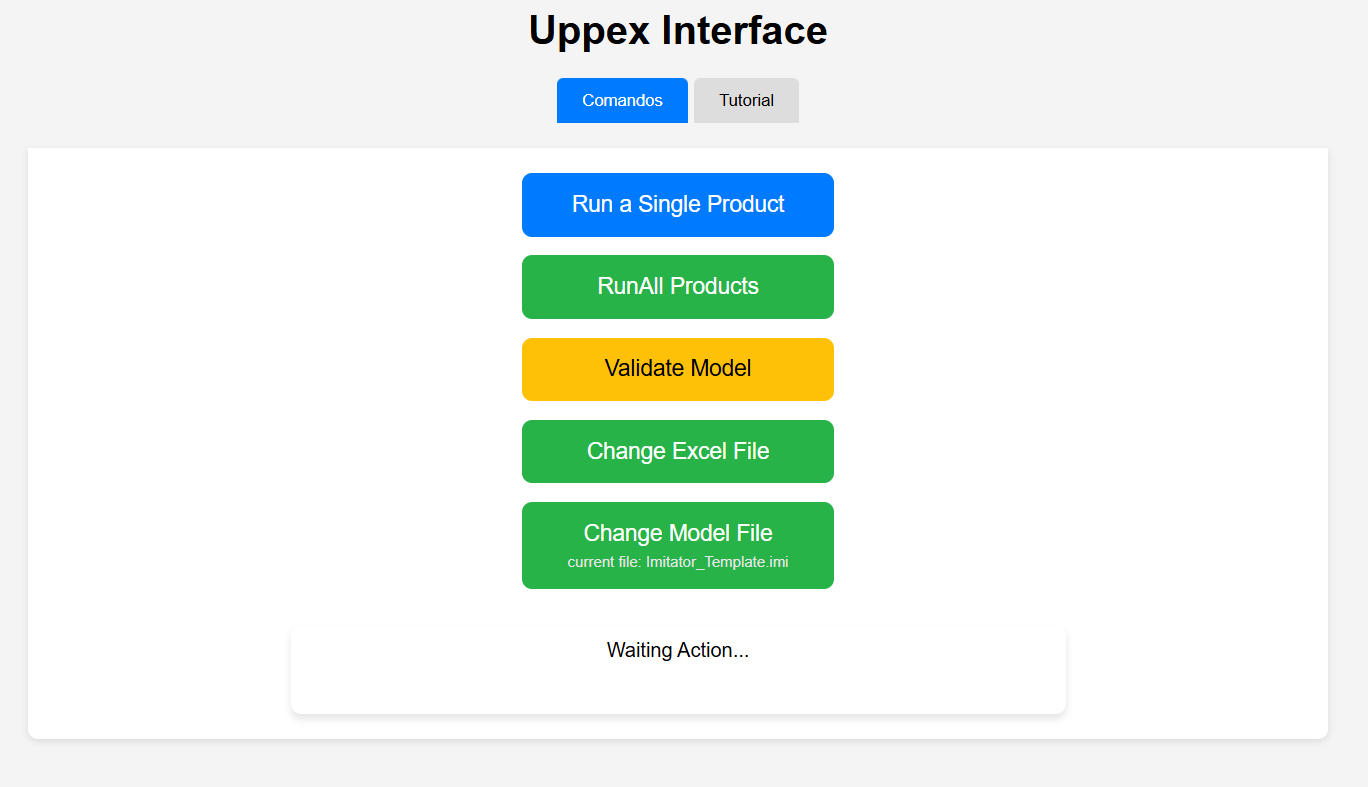
\includegraphics[width=\linewidth]{images/Interface.png}};
            \begin{scope}[x={(image1.south east)},y={(image1.north west)}]
                \draw[black, thick] (0,0) rectangle (1,1); % coordenadas normalizadas
            \end{scope}
        \end{tikzpicture}
        \caption{Uppex Interface Menu}
        \label{fig:UI}
    \end{minipage}
\end{figure}

It should be emphasized that, depending on the choice between Uppaal or Imitator in the menu shown in Figure \ref{fig:UI}, the file extension required for selection is automatically indicated in the final option, which also helps the user identify which file is being read. Additionally, there is a separate tab called \textit{Tutorial}, which, as the name suggests, guides the user step by step in interacting with the tool. Once the model is executed, a PDF report summarizing the results is opened immediately in a separate tab.




\chapter{Conclusions and future work}
%Conclusions and future work.

\section*{Conclusions}

Model checking is a complex task that consists of the automatic verification of properties in finite-state systems, such as elevators or vending machines. When applied to real-time systems, this task often becomes intractable due to the state explosion problem, leading to high computational costs. To address this issue, variations of the model are created, simplifying certain aspects depending on the system’s objectives, based on the theory of Software Product Lines. For this purpose, the Uppex tool is used, which, through a Microsoft Excel interface, reads the configurations selected by the user and builds an Uppaal model with small adjustments according to each configuration, also including the respective properties to be verified. As a result, it returns an HTML document summarizing the configurations, properties, and whether or not they were successfully verified.

The objective is to incorporate IMITATOR—a tool for the analysis and verification of real-time systems that also enables parameter synthesis—providing greater flexibility, optimization, and versatility to the system, as an additional backend and Model Checker within the Uppex tool. This objective was achieved through the changes made and demonstrated in Chapter 4. To test these modifications, the Worker-Hammer example was used, producing the expected results, notably the inclusion of parametric intervals in the output as well as the visual representation of the variations of the example model.

\section*{Prospect for future work}

As future work, there are several improvements that can be made:

\begin{itemize}

    \item The development of an user interface that encapsulates the current method of running the tool, which is currently done via command line. This would make it more appealing to professionals who are less familiar with the area, while also simplifying the selection of the model checker type and the choice of available options.

    \item Improvement of the report generated from the system analysis, particularly the visual representation of the models. Many of the model images are often repeated, and to make the report more compact and less extensive, one possible enhancement would be to group the images that are similar together.

\end{itemize}
		


\renewcommand{\baselinestretch}{1}
\bibliographystyle{plainnat}
% \bibliographystyle{alpha}
\bibliography{dissertation}
\printindex

\appendix
\renewcommand\chaptername{Appendix}

%\part{Appendices}

\chapter{Full Imitator code of the hammer example}

{\small
\begin{verbatim}
var
      session, t
           :clock;


      sessionTime,
      reactTime
           : parameter;


      nails
           : discrete;


      totalNails = 20
        : constant;




automaton Worker


synclabs: rest, hit, newNail, Work;

loc Rest: invariant session <= sessionTime - reactTime
      when True sync Work do {t := 0} goto Work;

loc Work: invariant session <= sessionTime && t <= reactTime
      when t >= reactTime sync newNail do {t := 0} goto Work;
      when t >= reactTime - 5 sync hit do {t := 0} goto Work;
      when session >= sessionTime sync rest do {session := 0} goto Rest;

end



automaton Hammer

synclabs: hit, newNail;

loc NailUp: invariant True
      when True sync hit goto NailHalf;

loc NailHalf: invariant True
      when countNails = True sync hit do {nails := nails +1} goto NailDone;

loc NailDone: invariant True
      when infiniteNails = True || nails <= totalNails sync newNail sync newNail goto Nailup;

end


init := 


        & loc[Worker] = Rest
        & loc[Hammer] = NailUp


        & session = 0
        & t = 0

    & nails = 0

    & sessionTime >= 0
    & reactTime >= 0


;


end
\end{verbatim}
}

\chapter{Running Imitator with the hammer example}

%explicar a secção

\begin{verbatim}
    
------------------------------------------------------------
Number of IPTAs                         : 2
Number of clocks                        : 2
Has invariants?                         : true
Has clocks with rate <>1?               : false
L/U subclass                            : U-PTA
Bounded parameters?                     : false
Has silent actions?                     : false
Is strongly deterministic?              : true
Number of parameters                    : 1
Number of discrete variables            : 1
Number of actions                       : 4
Total number of locations               : 5
Average locations per IPTA              : 2.5
Total number of transitions             : 7
Average transitions per IPTA            : 3.5
------------------------------------------------------------
\end{verbatim}

\begin{tcolorbox}[colframe=red]
\begin{verbatim}
BEGIN CONSTRAINT
 Parameter Constrain
END CONSTRAINT
\end{verbatim}
\end{tcolorbox}

\begin{verbatim}
------------------------------------------------------------
Constraint soundness                    : exact
Termination                             : regular termination
Constraint nature                       : good
------------------------------------------------------------
Number of states                        : 1
Number of transitions                   : 0
Number of computed states               : 2
Total computation time                  : 0.007 second
States/second in state space            : 128.6 (1/0.007 second)
Computed states/second                  : 257.2 (2/0.007 second)
Estimated memory                        : 2.078 MiB (i.e., 272498 words of size 8)
------------------------------------------------------------

------------------------------------------------------------
 Statistics: Algorithm counters
------------------------------------------------------------
main algorithm + parsing                : 0.043 second
main algorithm                          : 0.014 second
------------------------------------------------------------
 Statistics: Parsing counters
------------------------------------------------------------
model parsing and converting            : 0.025 second
------------------------------------------------------------
 Statistics: State computation counters
------------------------------------------------------------
number of state comparisons             : 0
number of constraints comparisons       : 0
number of new states <= old             : 0
number of new states >= old             : 0
StateSpace.merging attempts             : 0
StateSpace.merges                       : 0
------------------------------------------------------------
 Statistics: Graphics-related counters
------------------------------------------------------------
state space drawing                     : 0.000 second
------------------------------------------------------------
 Statistics: Global counter
------------------------------------------------------------
total                                   : 0.050 second
\end{verbatim}

\chapter{Uppex HTML Coffee Result}

\begin{figure}[H]
    \centering
    \begin{minipage}{\textwidth}
        \centering
        \begin{tikzpicture}
            \node[anchor=south west,inner sep=0] (image1) at (0,0) {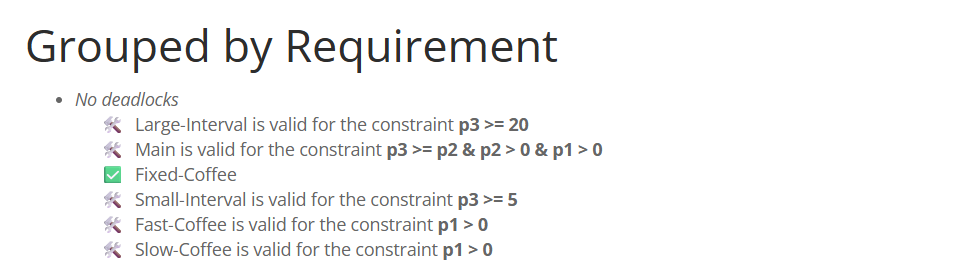
\includegraphics[width=\linewidth]{images/fixed_end.png}};
            \begin{scope}[x={(image1.south east)},y={(image1.north west)}]
                \draw[black, thick] (0,0) rectangle (1,1); % coordenadas normalizadas
            \end{scope}
        \end{tikzpicture}
        \caption{Grouped by Requerimets Report Result}
        \label{fig:Fixed_C}
    \end{minipage}
\end{figure}

\begin{figure}[H]
    \centering
    \begin{minipage}{\textwidth}
        \centering
        \begin{tikzpicture}
            \node[anchor=south west,inner sep=0] (image1) at (0,0) {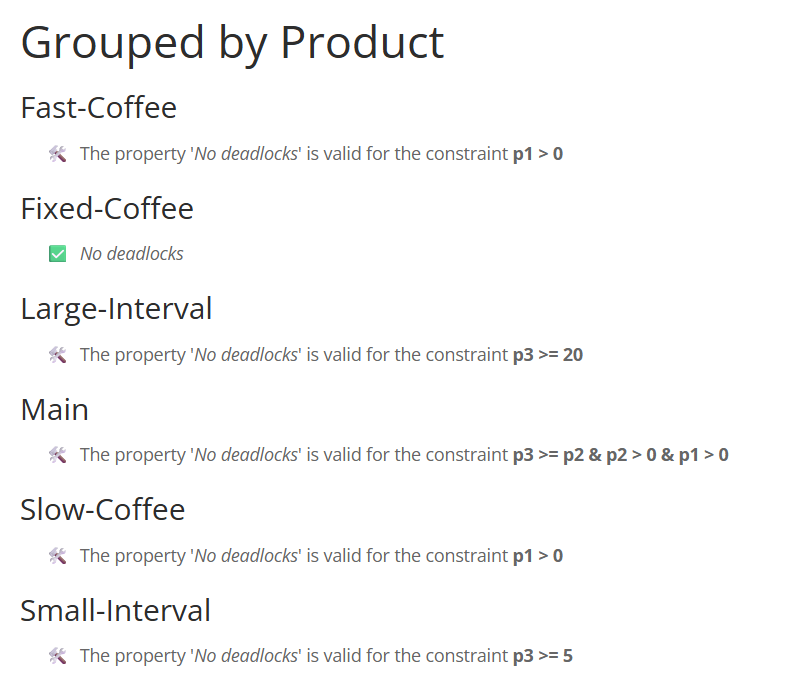
\includegraphics[width=\linewidth]{images/Grouped.png}};
            \begin{scope}[x={(image1.south east)},y={(image1.north west)}]
                \draw[black, thick] (0,0) rectangle (1,1); % coordenadas normalizadas
            \end{scope}
        \end{tikzpicture}
        \caption{Grouped by Requerimets Report Result}
        \label{fig:Fixed_G}
    \end{minipage}
\end{figure}

\begin{figure}[H]
    \centering
    \begin{minipage}{\textwidth}
        \centering
        \begin{tikzpicture}
            \node[anchor=south west,inner sep=0] (image1) at (0,0) {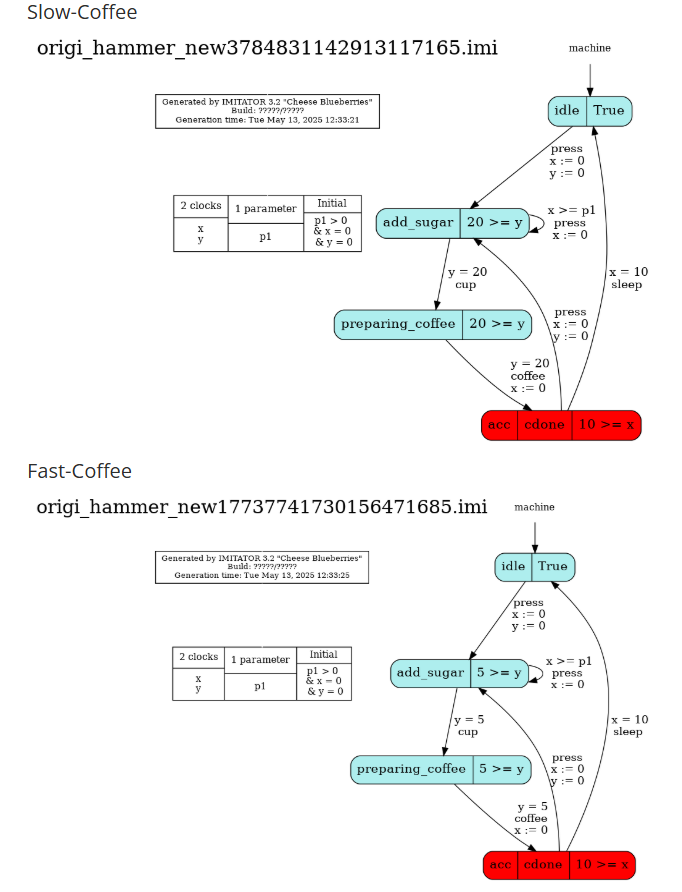
\includegraphics[width=\linewidth]{images/im1.png}};
            \begin{scope}[x={(image1.south east)},y={(image1.north west)}]
                \draw[black, thick] (0,0) rectangle (1,1); % coordenadas normalizadas
            \end{scope}
        \end{tikzpicture}
        \caption{Coffee Automata Products Part 1 Report Result}
        \label{fig:Fixed_im1}
    \end{minipage}
\end{figure}

\begin{figure}[H]
    \centering
    \begin{minipage}{\textwidth}
        \centering
        \begin{tikzpicture}
            \node[anchor=south west,inner sep=0] (image1) at (0,0) {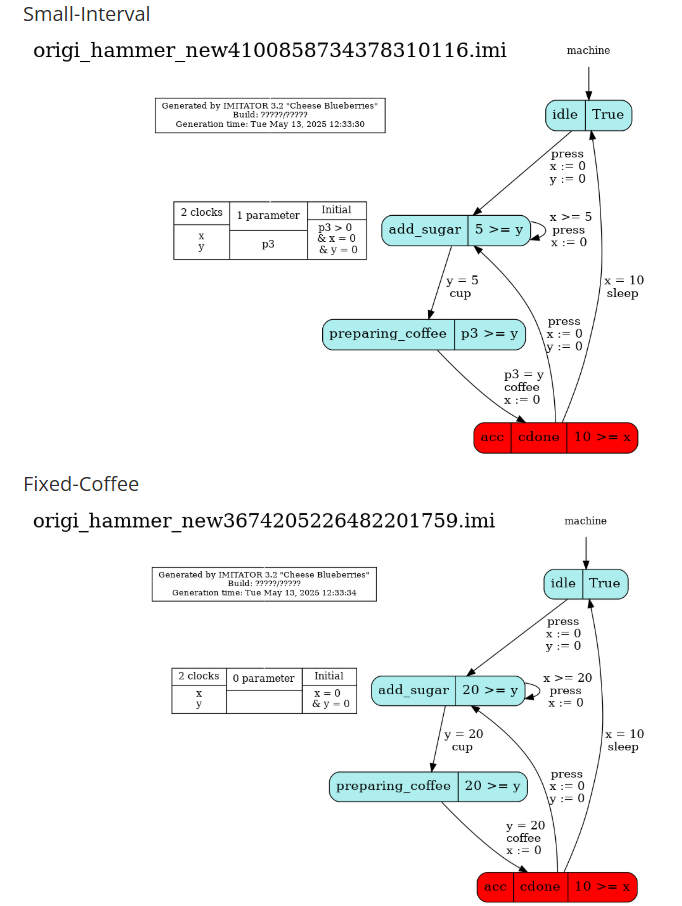
\includegraphics[width=\linewidth]{images/im2.png}};
            \begin{scope}[x={(image1.south east)},y={(image1.north west)}]
                \draw[black, thick] (0,0) rectangle (1,1); % coordenadas normalizadas
            \end{scope}
        \end{tikzpicture}
        \caption{Coffee Automata Products Part 2 Report Result}
        \label{fig:Fixed_im2}
    \end{minipage}
\end{figure}

\begin{figure}[H]
    \centering
    \begin{minipage}{\textwidth}
        \centering
        \begin{tikzpicture}
            \node[anchor=south west,inner sep=0] (image1) at (0,0) {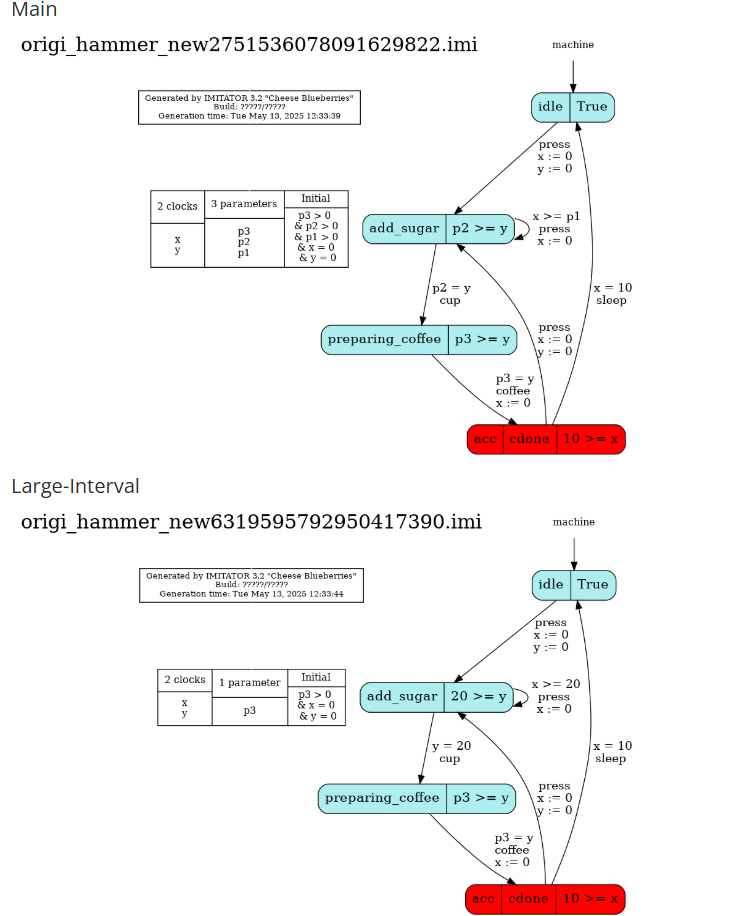
\includegraphics[width=\linewidth]{images/im3.png}};
            \begin{scope}[x={(image1.south east)},y={(image1.north west)}]
                \draw[black, thick] (0,0) rectangle (1,1); % coordenadas normalizadas
            \end{scope}
        \end{tikzpicture}
        \caption{Coffee Automata Products Part 3 Report Result}
        \label{fig:Fixed_im3}
    \end{minipage}
\end{figure}


\chapter{Uppex HTML Hammer Result}
%colocar link

\begin{figure}[H]
    \centering
    \begin{minipage}{\textwidth}
        \centering
        \begin{tikzpicture}
            \node[anchor=south west,inner sep=0] (image1) at (0,0) {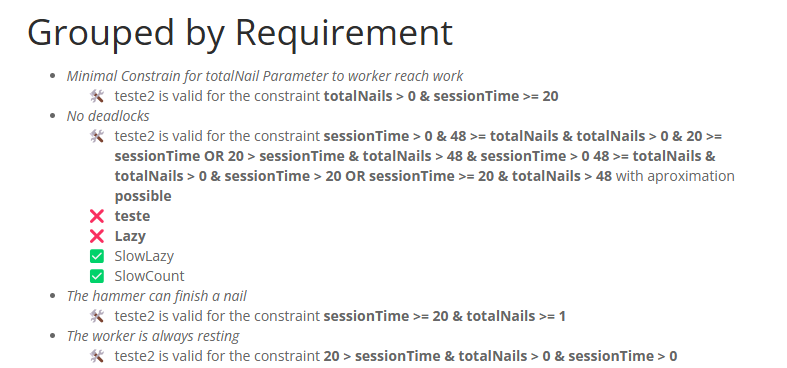
\includegraphics[width=\linewidth]{images/res1.png}};
            \begin{scope}[x={(image1.south east)},y={(image1.north west)}]
                \draw[black, thick] (0,0) rectangle (1,1); % coordenadas normalizadas
            \end{scope}
        \end{tikzpicture}
        \caption{Grouped by Product Coffee Report Result}
        \label{fig:GR}
    \end{minipage}
\end{figure}

\begin{figure}[H]
    \centering
    \begin{minipage}{\textwidth}
        \centering
        \begin{tikzpicture}
            \node[anchor=south west,inner sep=0] (image1) at (0,0) {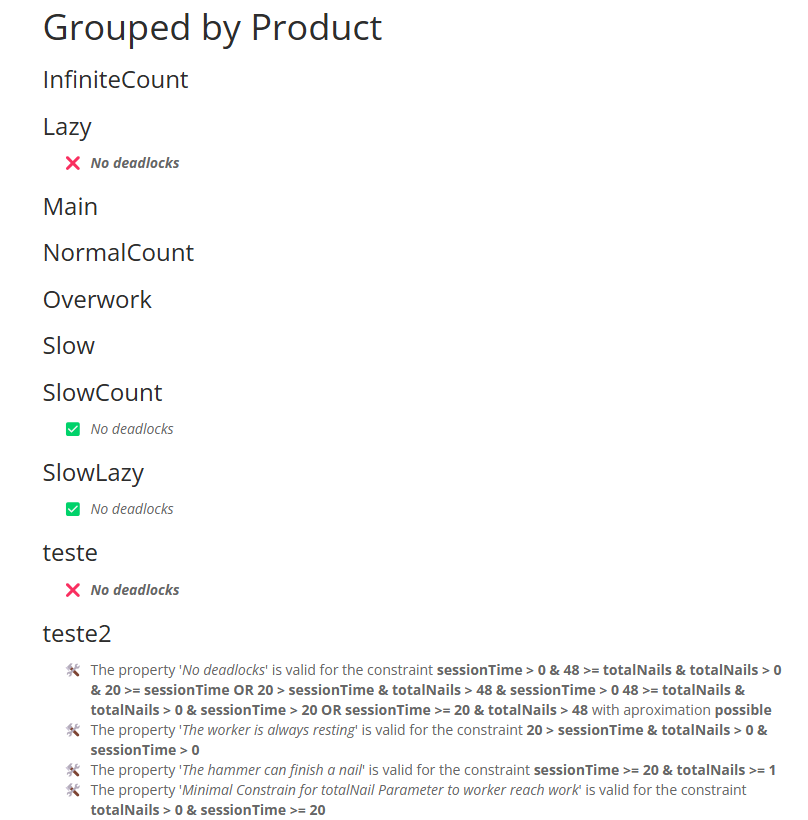
\includegraphics[width=\linewidth]{images/res2.png}};
            \begin{scope}[x={(image1.south east)},y={(image1.north west)}]
                \draw[black, thick] (0,0) rectangle (1,1); % coordenadas normalizadas
            \end{scope}
        \end{tikzpicture}
        \caption{Grouped by Product Report Result}
        \label{fig:GP}
    \end{minipage}
\end{figure}

\begin{figure}[H]
    \centering
    \begin{minipage}{\textwidth}
        \centering
        \begin{tikzpicture}
            \node[anchor=south west,inner sep=0] (image1) at (0,0) {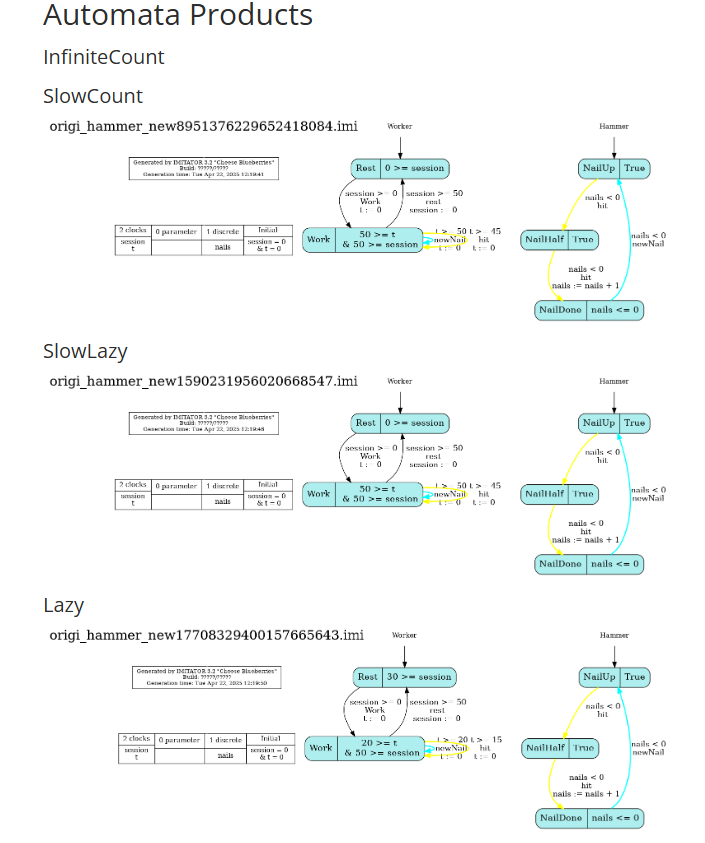
\includegraphics[width=\linewidth]{images/res3.png}};
            \begin{scope}[x={(image1.south east)},y={(image1.north west)}]
                \draw[black, thick] (0,0) rectangle (1,1); % coordenadas normalizadas
            \end{scope}
        \end{tikzpicture}
        \caption{Automata Products Part 1 Report Result}
        \label{fig:AP1}
    \end{minipage}
\end{figure}

\begin{figure}[H]
    \centering
    \begin{minipage}{\textwidth}
        \centering
        \begin{tikzpicture}
            \node[anchor=south west,inner sep=0] (image1) at (0,0) {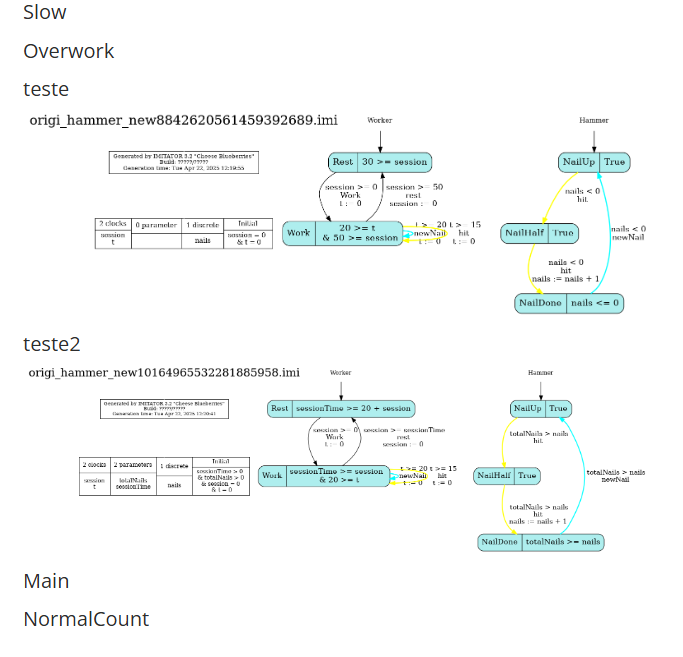
\includegraphics[width=\linewidth]{images/res4.png}};
            \begin{scope}[x={(image1.south east)},y={(image1.north west)}]
                \draw[black, thick] (0,0) rectangle (1,1); % coordenadas normalizadas
            \end{scope}
        \end{tikzpicture}
        \caption{Automata Products Part 2 Report Result}
        \label{fig:AP2}
    \end{minipage}
\end{figure}






%%\chapter{Details of results}
         
%%\chapter{Listings}
	
%%\chapter{Tooling}


\pagestyle{empty}
\cleartoevenpage
\null
\thispagestyle{empty}
\pagecolor{PANTONECoolGray7C}
\afterpage{\nopagecolor}
\newpage

\begin{backcover}
\thispagestyle{empty}{~\vfill
\noindent

\vfill ~}
\end{backcover}



\end{document}
